%% SUMMARY OF CHANGE POINT ANALYSIS (CPA) FOR CASE DATASET
% ----------------------------------------------------- set up ---------------------------------------------------------------
\documentclass[11pt, letterpaper]{article}
\usepackage{graphicx}
\graphicspath{{Users/Lucy/Documents/Berlin/FU/MCNB/Praktikum/MPI_MBE/AffectiveVR/Phase1/CASE/results/cpa/}{sub_1/}{all_data/}{all/}}
\usepackage{caption}
\usepackage{subcaption}
\usepackage{hyperref}
\hypersetup{
    colorlinks=true,
    linkcolor=blue,
    filecolor=magenta,      
    urlcolor=cyan,
    pdftitle={cpa_case},
    pdfpagemode=FullScreen,
    }
\urlstyle{same}
\usepackage[utf8]{inputenc}
\usepackage{float}

% ----------------------------------------------------- title ---------------------------------------------------------------
\title{Change Point Analysis (CPA) of the CASE Dataset}
\author{Lucy Roellecke}
\date{22 November 2023}
\begin{document}
\maketitle

% ----------------------------------------------------- abstract ---------------------------------------------------------------
\begin{abstract}
This document summarizes the results of performing a change point analysis (CPA) of the textit{Dataset of continuous affect annnotations and physiological signals for emotion analysis (CASE}, available here: \url{https://springernature.figshare.com/collections/A_dataset_of_continuous_affect_annotations_and_physiological_signals_for_emotion_analysis/4260668}). The results reported in this document are in line with the results found by the original authors. Qualitatively meaningful change points in the participants' annotation data can be detected using a data-driven approach such as the CPA easily for highly arousing, negative videos (such as scary videos) but are harder to detect in low arousing and positively valenced videos. Interindividual differences are are high in all conditions.
\end{abstract}

\newpage

% ----------------------------------------------------- analysis notes ---------------------------------------------------------------
\section{Analysis Notes}
The change point analysis was undertaken by using the Python package \verb|ruptures| (Version 1.1.8) and the algorithm of linearly penalized segmentation (\verb|Pelt|). The parameters of the algorithm were set as follows: \verb|model=l2| (least squared deviation model),  \verb|jump=5| (controls the grid of possible change points), and \verb|pen=1| (the optimal penalization factor was determined by visual inspection of an elbow plot with possible penalty values on the x-axis and the resulting number of change points on the y-axis). \verb|cpa.py| performs a change point analysis for each participant separately, while \verb|cpa_average.py| performs a change point analysis for the annotation data averaged across all participants. Both scripts return csv files with the x-(time)-coordinates of the change points and the number of change points, and plot the timeseries together with the change points as dashed lines for each of the 8 stimuli videos separately (see \ref{results}). The latter script performs different kinds of visualization: 1) Plotting the averaged timeseries and the averaged change points; 2) Plotting all timeseries of all participants and the averaged change points; 3) Plotting the averaged timeseries and all change points for all participants. See \ref{results} for the different visualizations. For code and figure availability, see section \ref{code}.

% ----------------------------------------------------- descriptive results ---------------------------------------------------------------
\section{Descriptive Results} \label{results}

% +++++ subsection individual cpa ++++++
\subsection{CPA for each participant separately}
Figure \ref{fig:sub1} shows the change points identified for each video's arousal and valence ratings for subject 1 (as an example). The algorithm seems to be able to identify abrupt decreases and increase in the emotion ratings.

% figure cpa of subject 1
\begin{figure}
    \centering
    \begin{subfigure}[t]{0.49\textwidth}
        \centering
        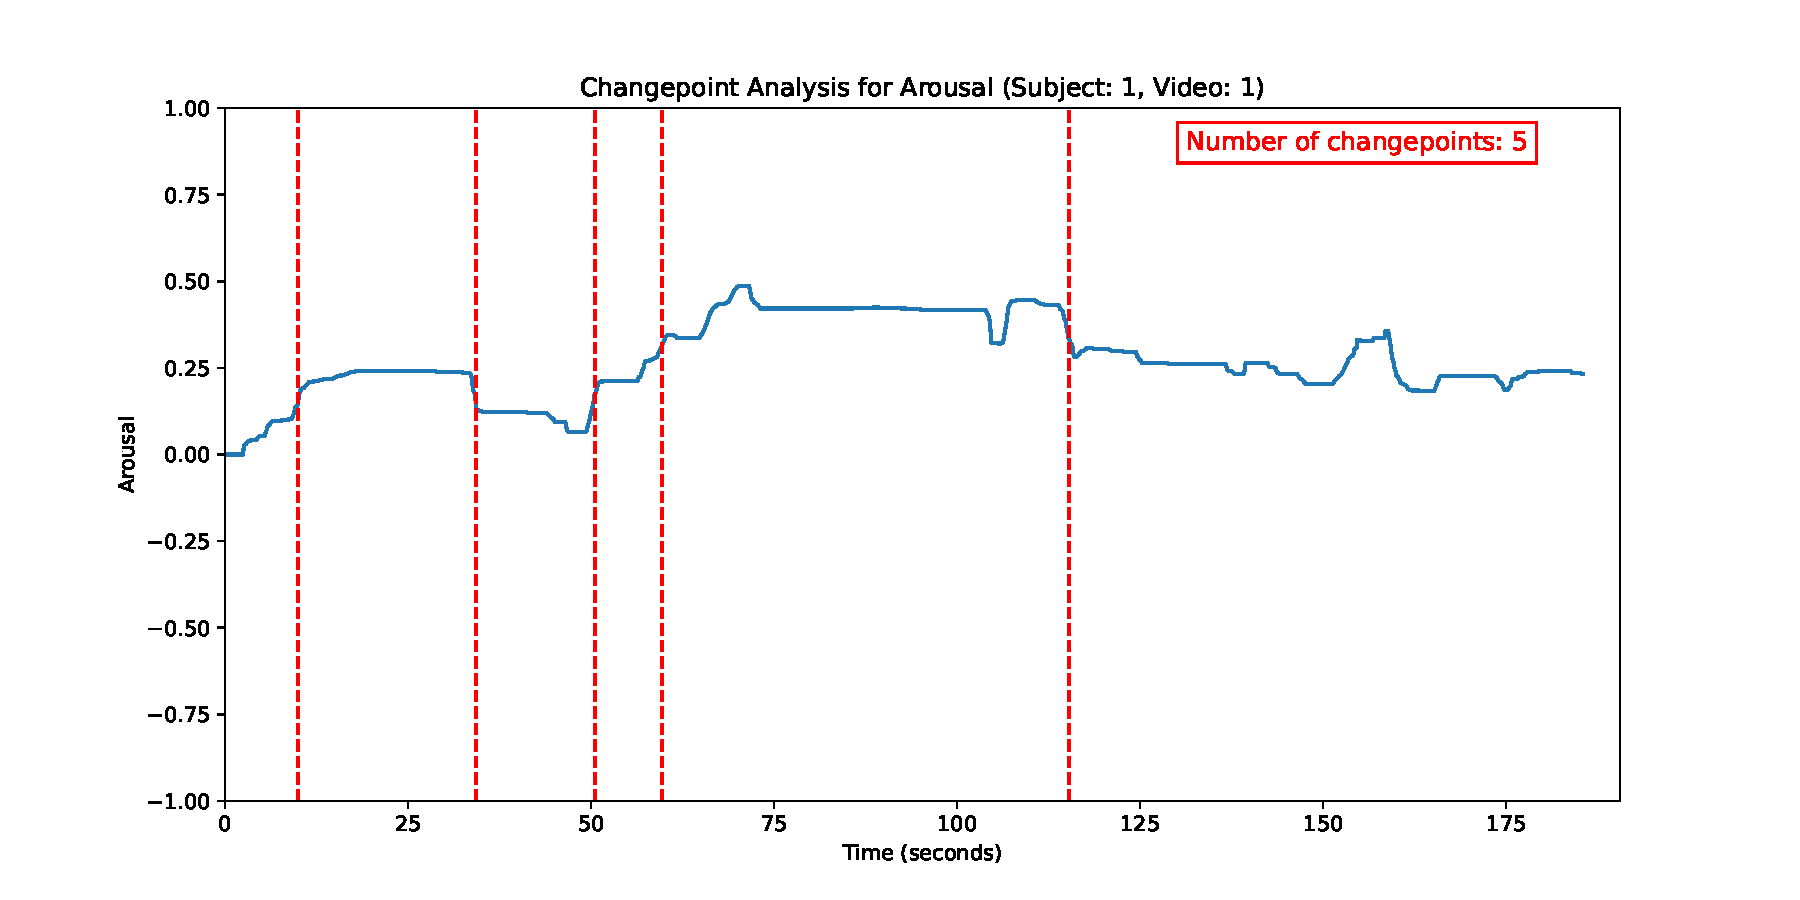
\includegraphics[width=\linewidth]{sub_1_changepoints_V1_arousal} 
        \caption{} \label{fig:sub_1_changepoints_V1_arousal}
    \end{subfigure}
    \hfill
    \begin{subfigure}[t]{0.49\textwidth}
        \centering
        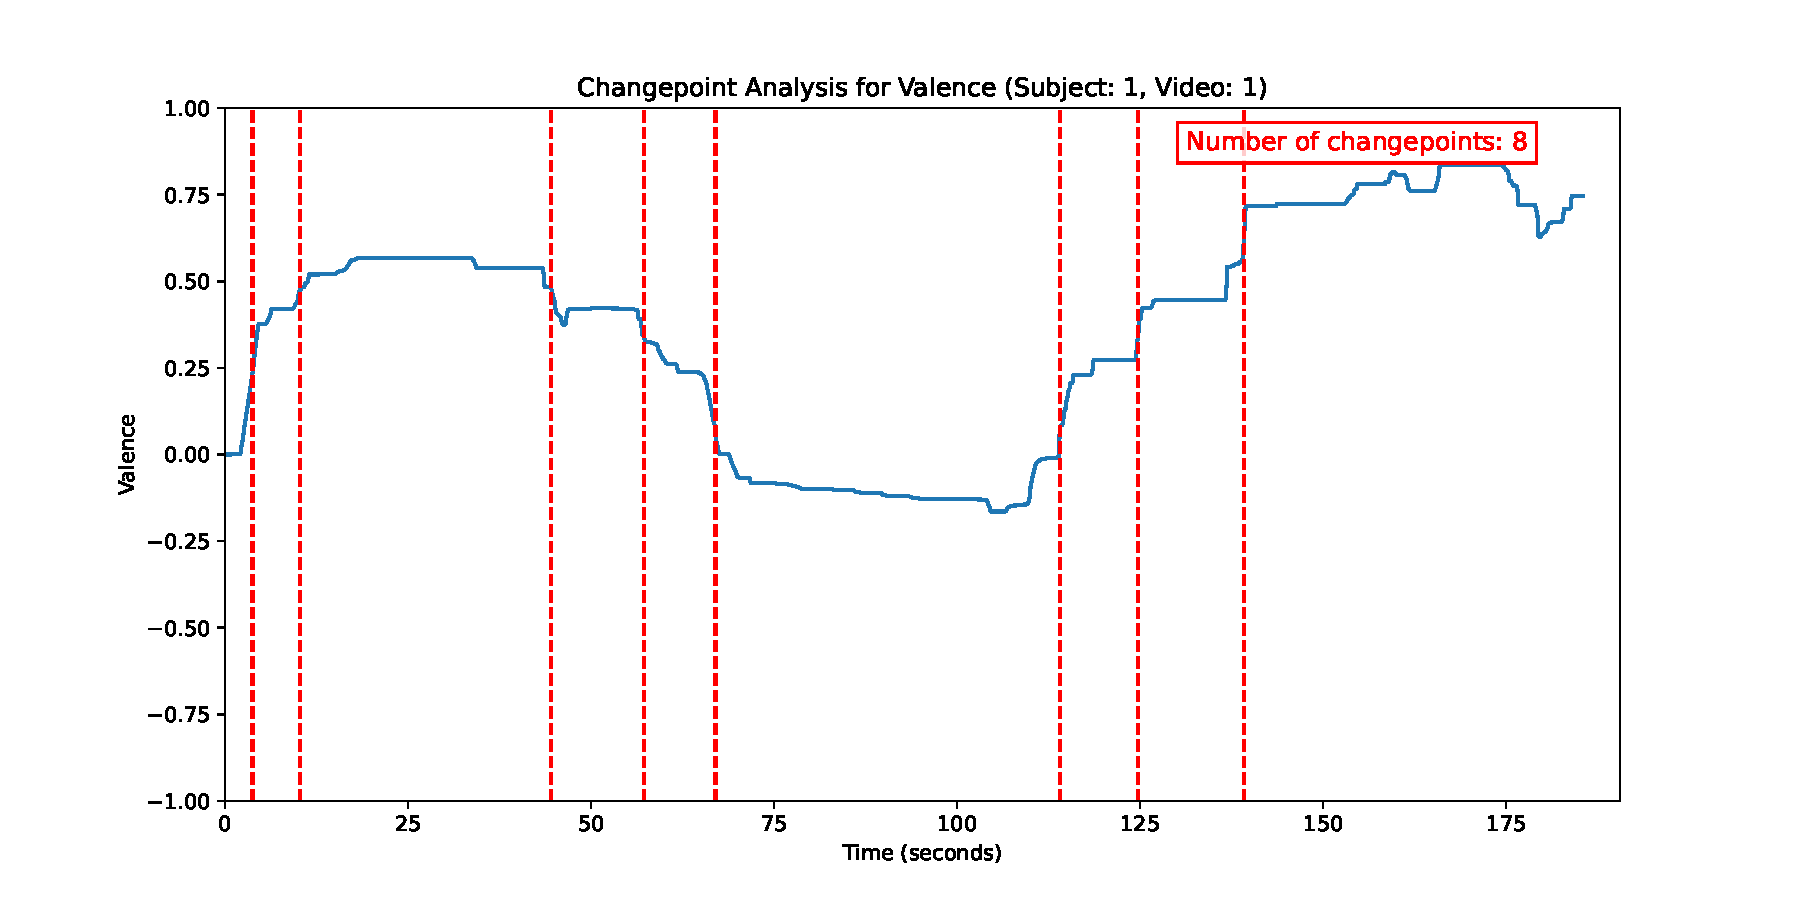
\includegraphics[width=\linewidth]{sub_1_changepoints_V1_valence} 
        \caption{} \label{fig:sub_1_changepoints_V1_valence}
    \end{subfigure}

    \vspace{1cm}
    
    \centering
    \begin{subfigure}[t]{0.49\textwidth}
        \centering
        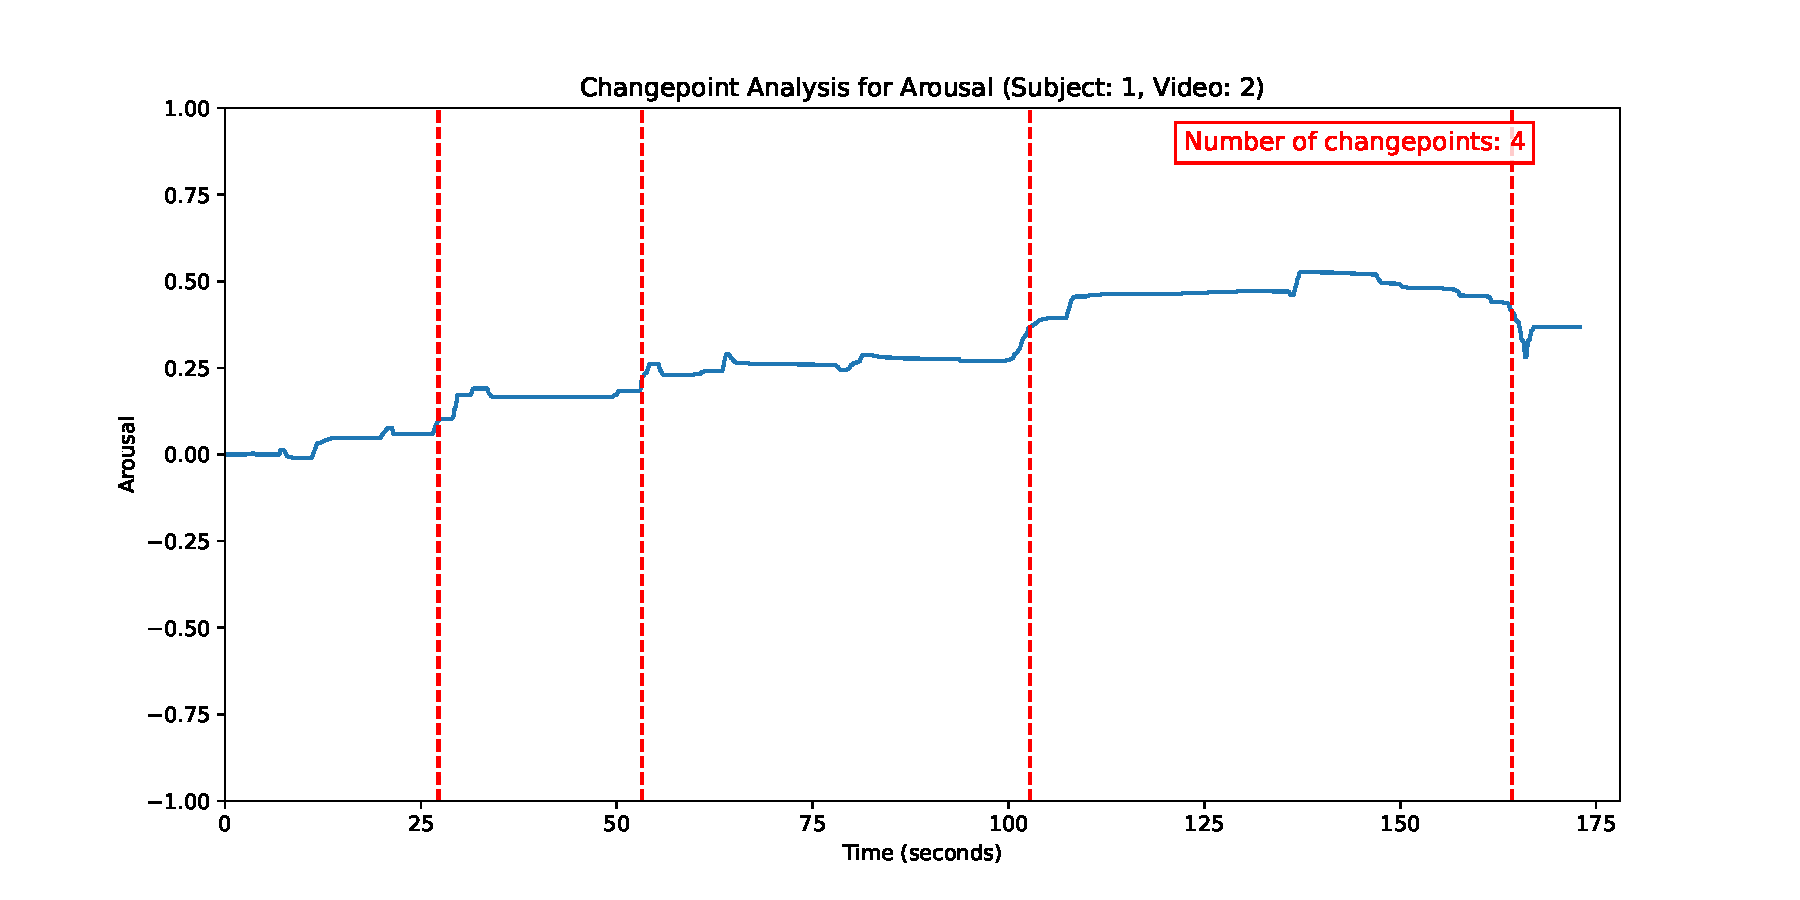
\includegraphics[width=\linewidth]{sub_1_changepoints_V2_arousal} 
        \caption{} \label{fig:sub_1_changepoints_V2_arousal}
    \end{subfigure}
    \hfill
    \begin{subfigure}[t]{0.49\textwidth}
        \centering
        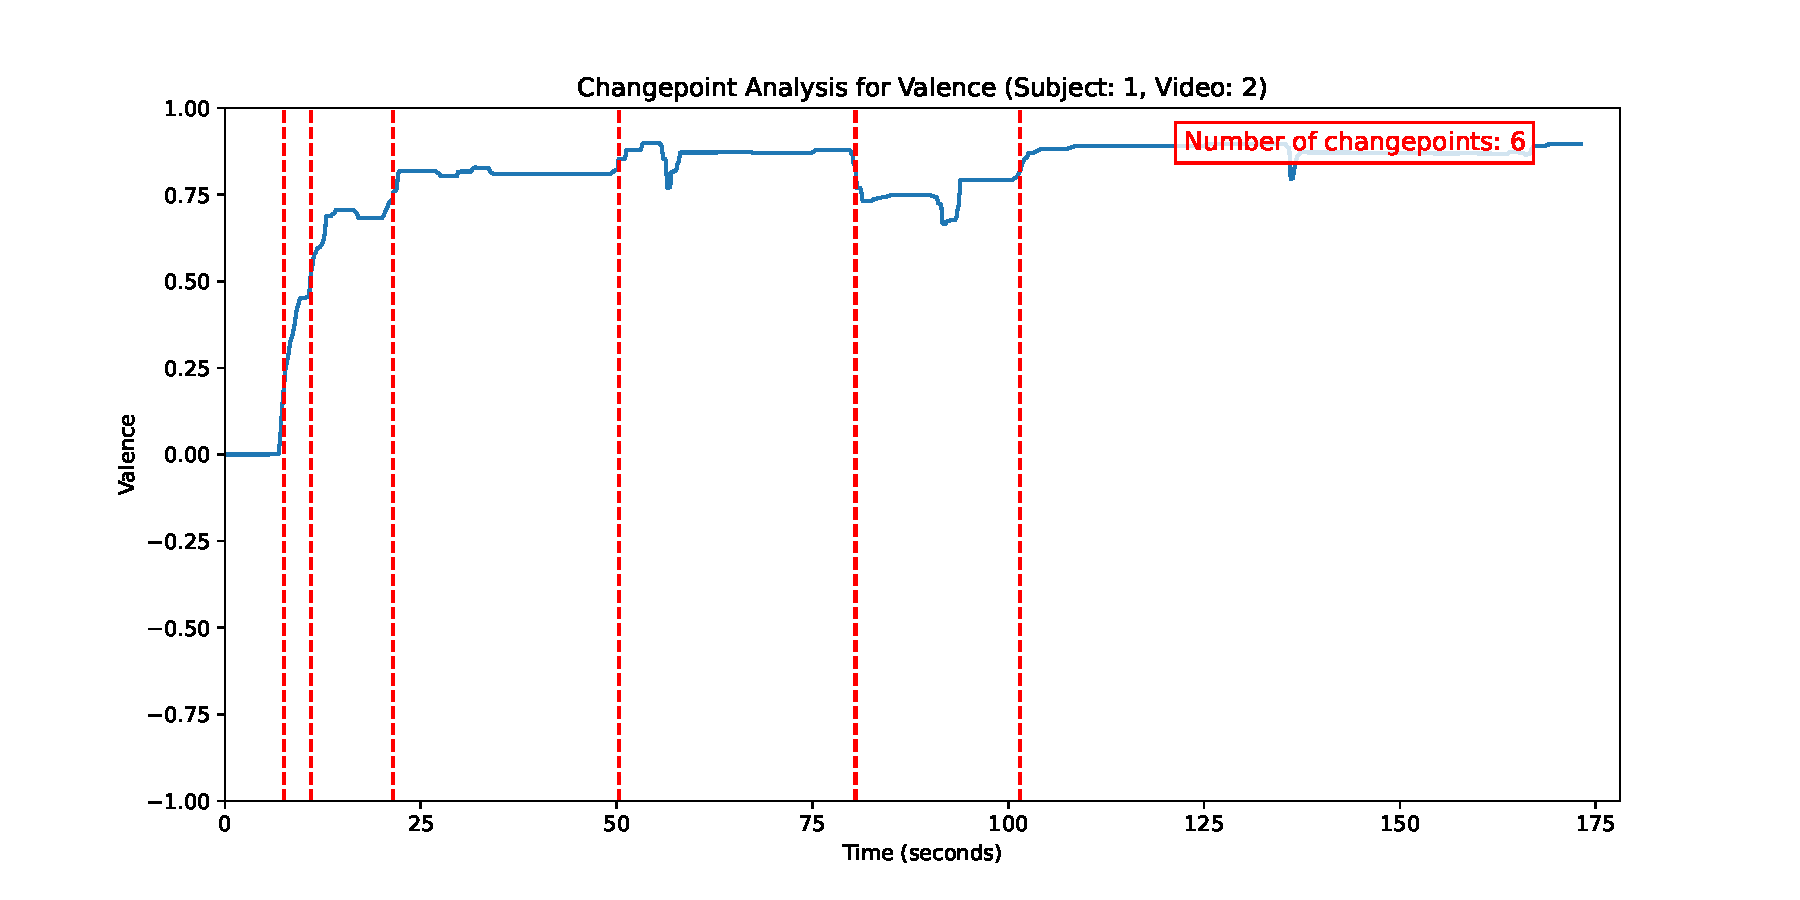
\includegraphics[width=\linewidth]{sub_1_changepoints_V2_valence} 
        \caption{} \label{fig:sub_1_changepoints_V2_valence}
    \end{subfigure}
    
        \centering
    \begin{subfigure}[t]{0.49\textwidth}
        \centering
        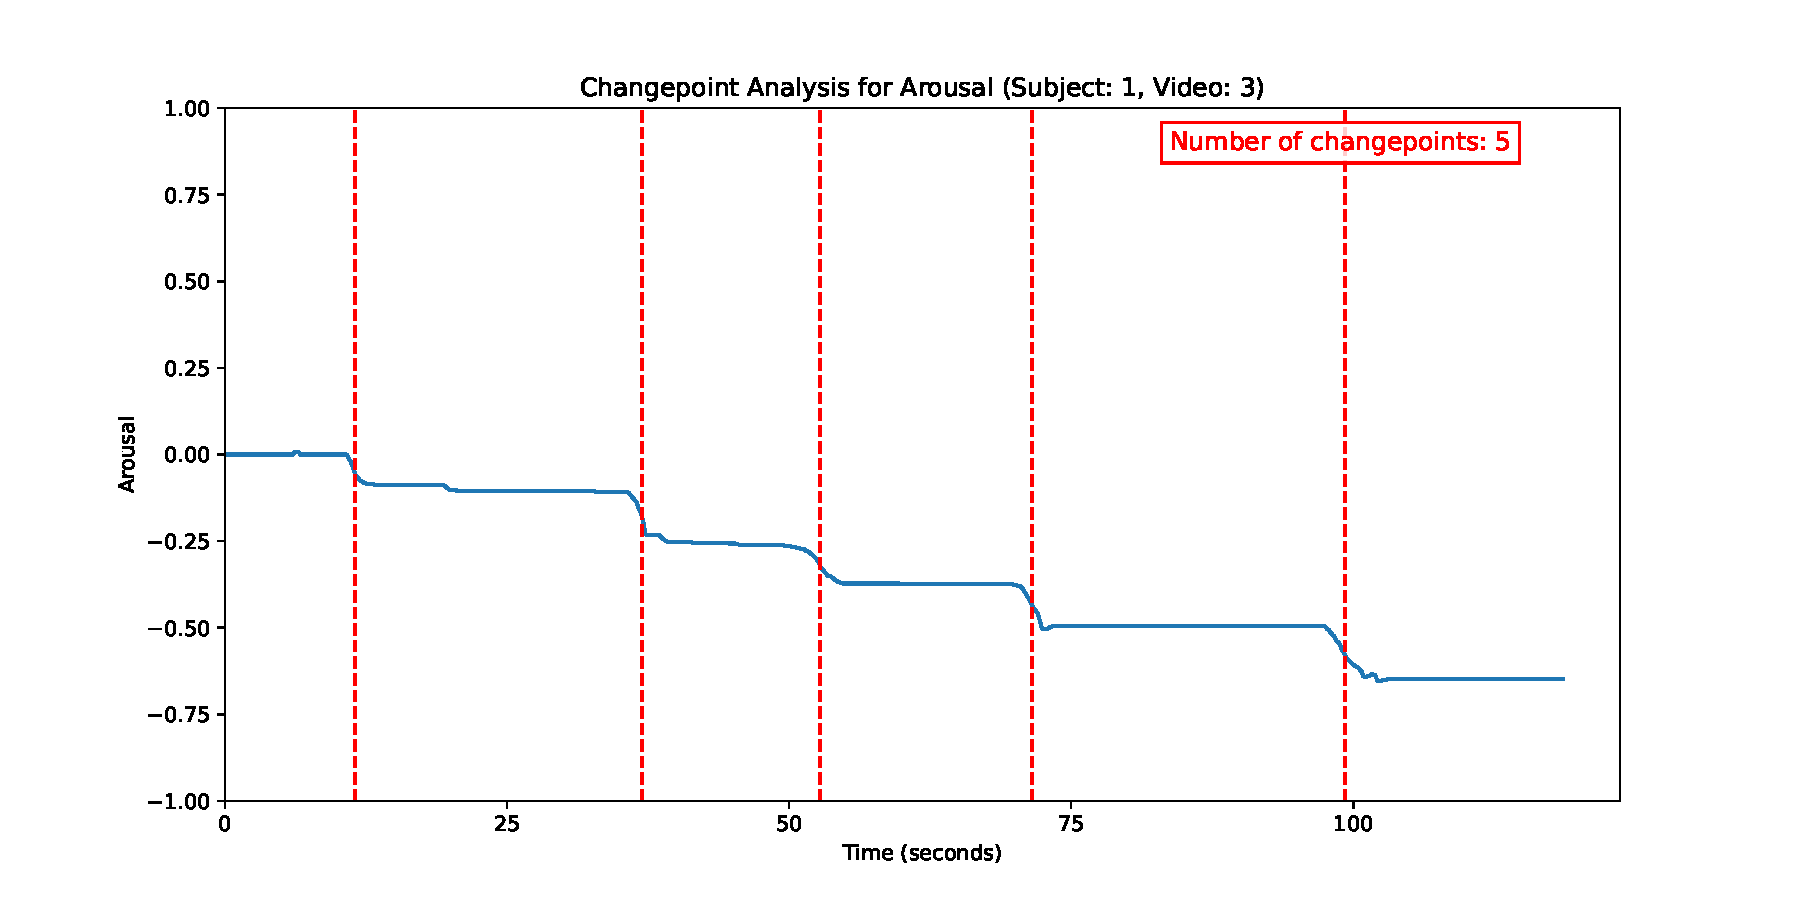
\includegraphics[width=\linewidth]{sub_1_changepoints_V3_arousal} 
        \caption{} \label{fig:sub_1_changepoints_V3_arousal}
    \end{subfigure}
    \hfill
    \begin{subfigure}[t]{0.49\textwidth}
        \centering
        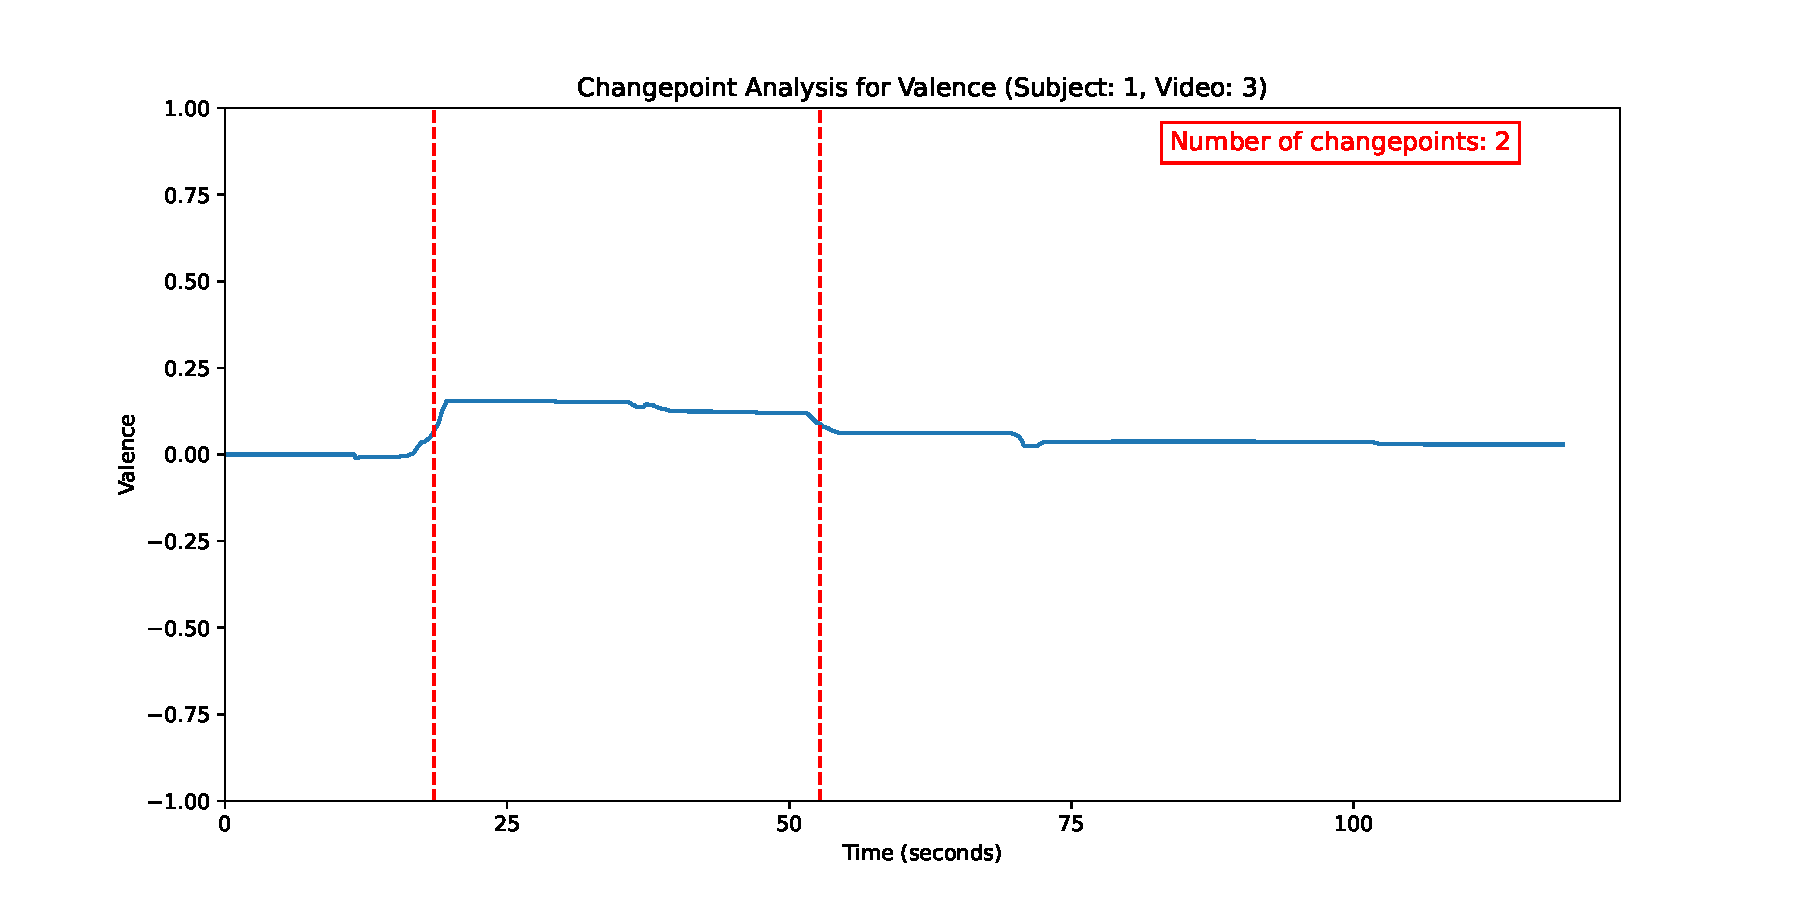
\includegraphics[width=\linewidth]{sub_1_changepoints_V3_valence} 
        \caption{} \label{fig:sub_1_changepoints_V3_valence}
    \end{subfigure}

    \vspace{1cm}
    
        \centering
    \begin{subfigure}[t]{0.49\textwidth}
        \centering
        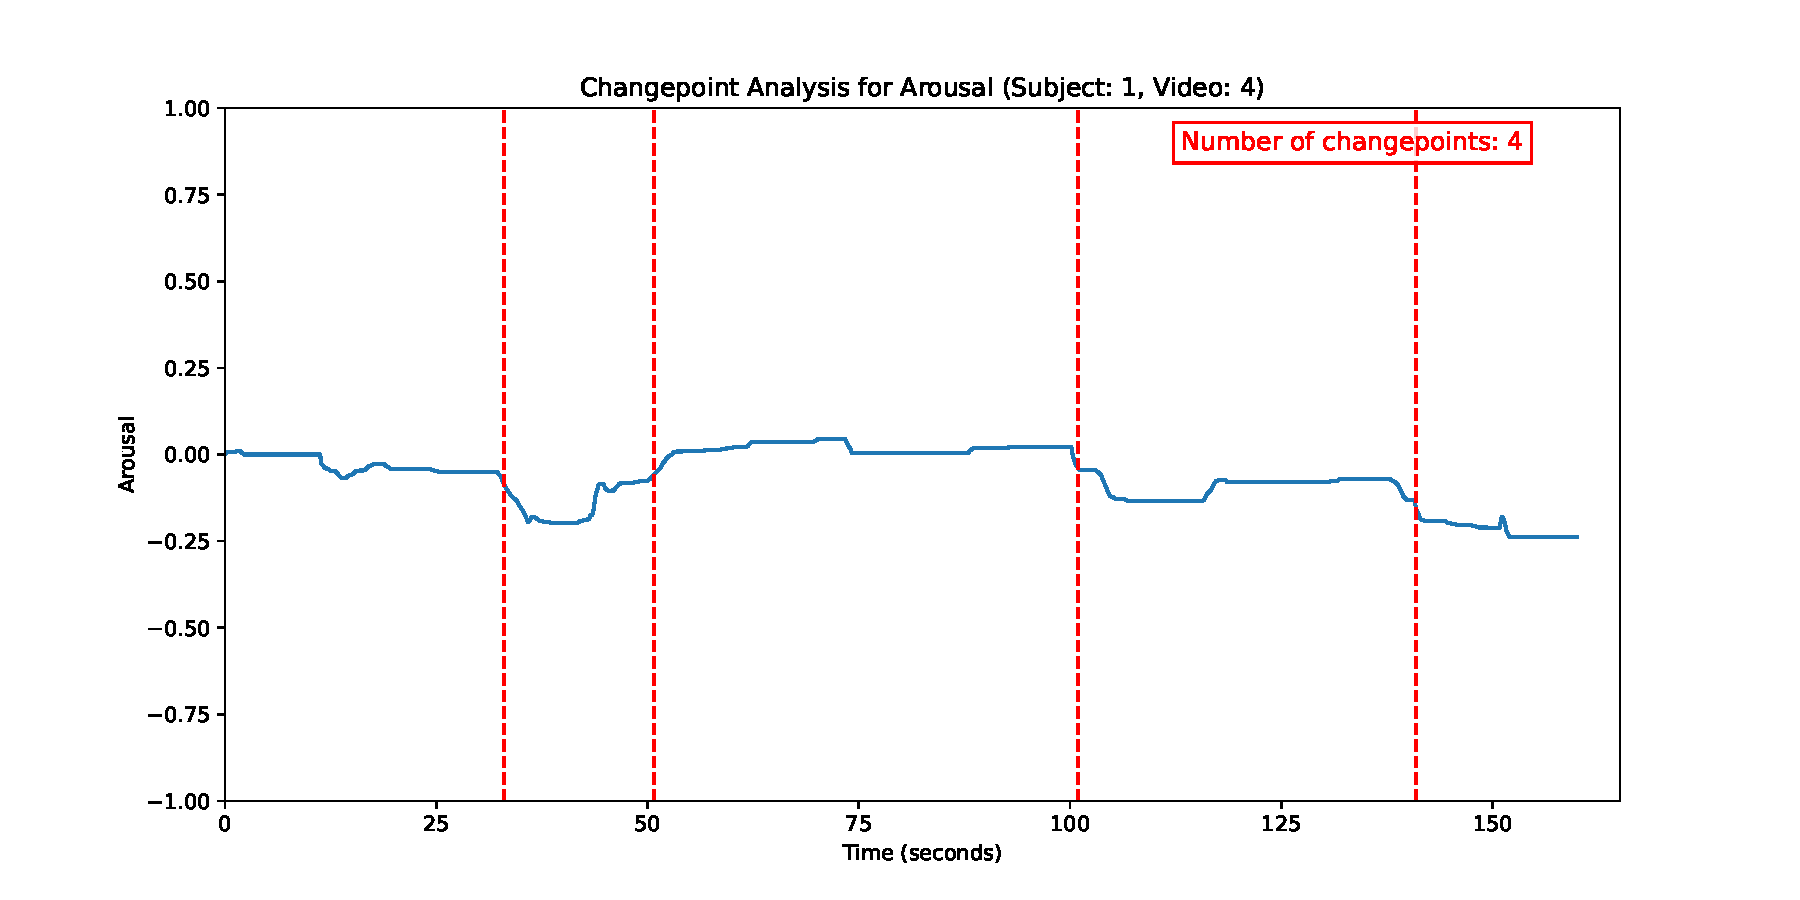
\includegraphics[width=\linewidth]{sub_1_changepoints_V4_arousal} 
        \caption{} \label{fig:sub_1_changepoints_V4_arousal}
    \end{subfigure}
    \hfill
    \begin{subfigure}[t]{0.49\textwidth}
        \centering
        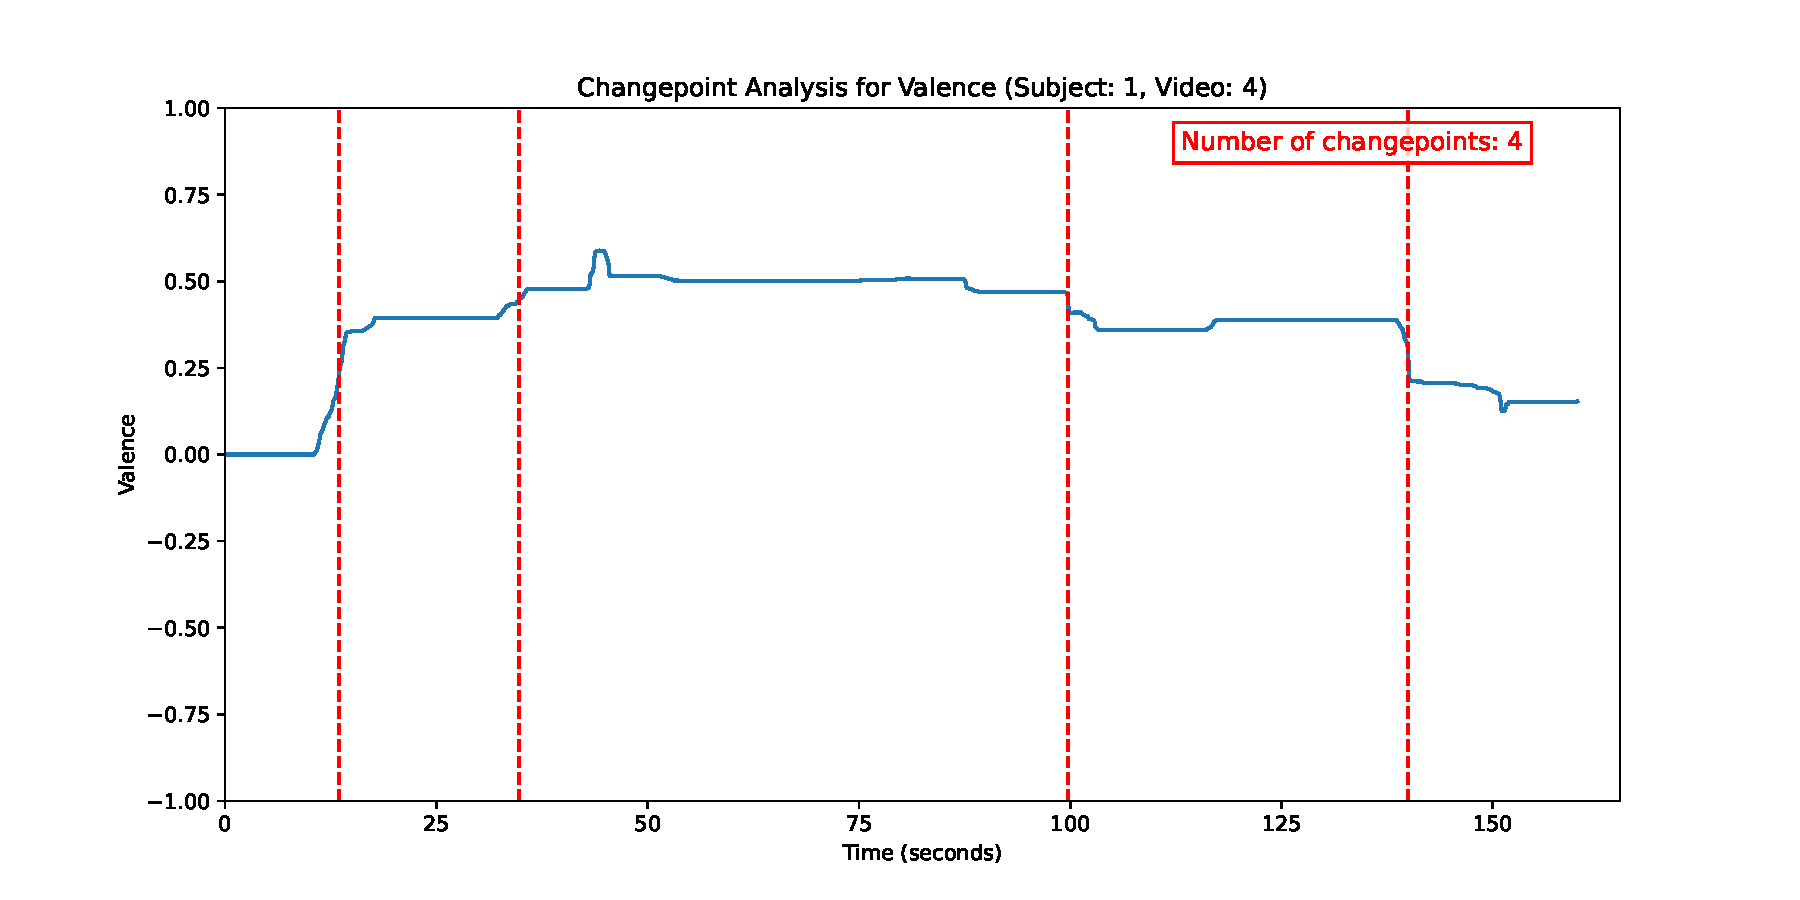
\includegraphics[width=\linewidth]{sub_1_changepoints_V4_valence} 
        \caption{} \label{fig:sub_1_changepoints_V4_valence}
    \end{subfigure}
\end{figure}

\begin{figure} \ContinuedFloat
        \centering
    \begin{subfigure}[t]{0.49\textwidth}
        \centering
        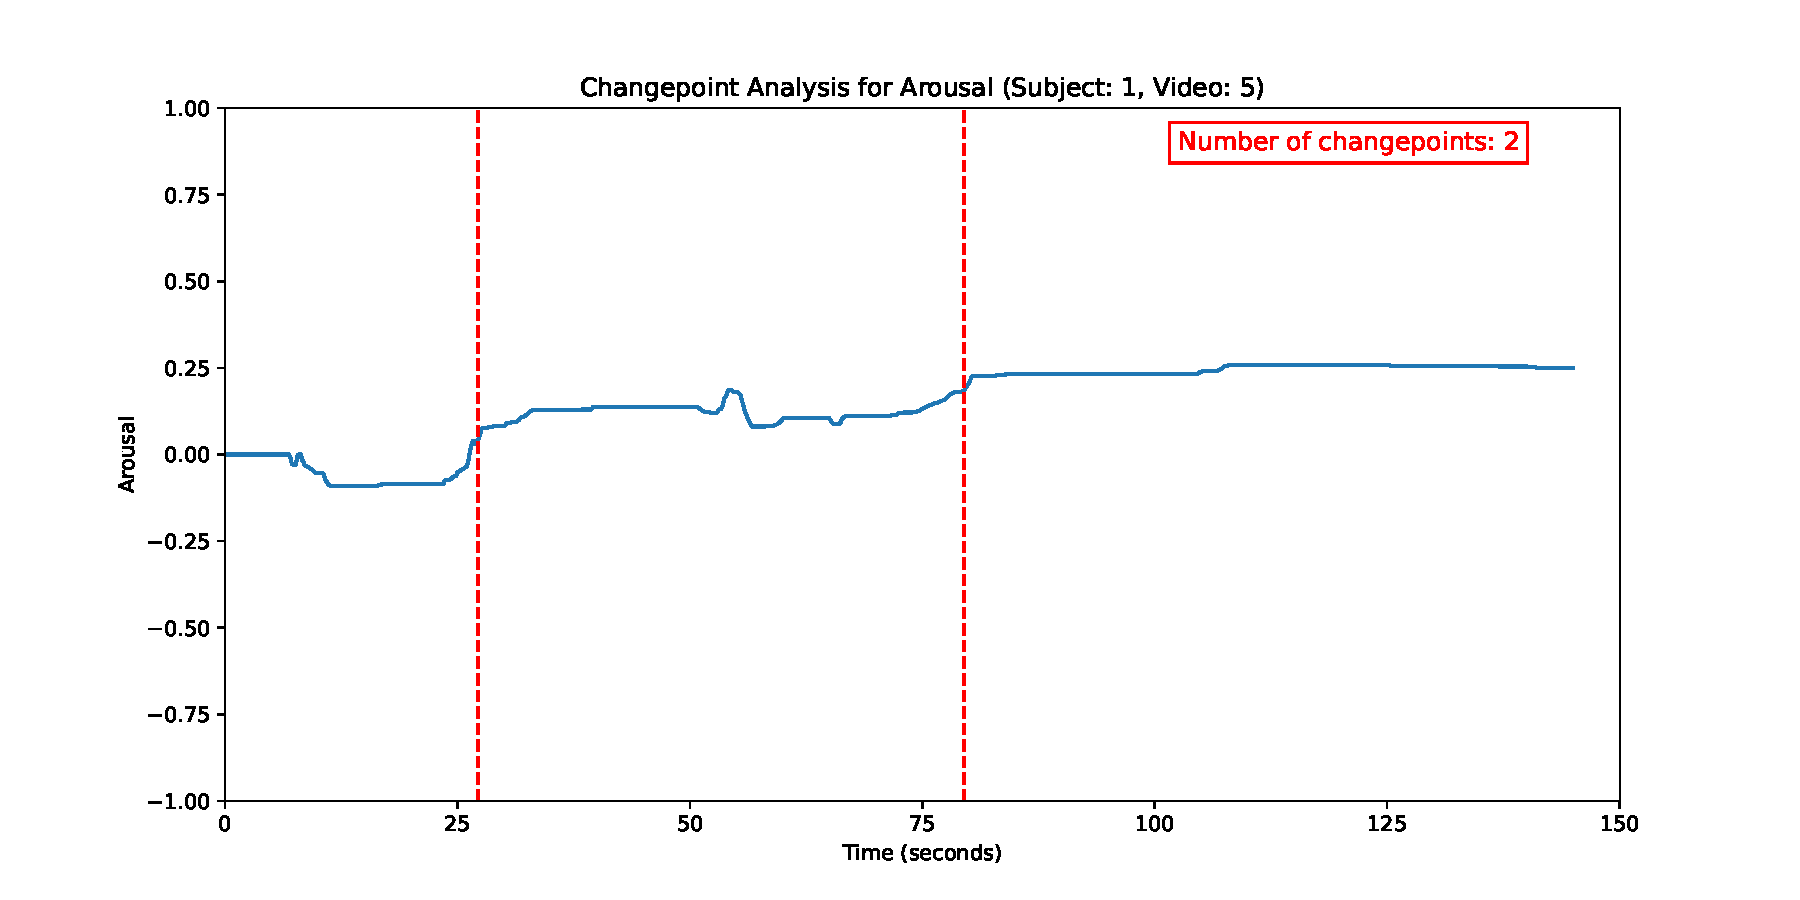
\includegraphics[width=\linewidth]{sub_1_changepoints_V5_arousal} 
        \caption{} \label{fig:sub_1_changepoints_V5_arousal}
    \end{subfigure}
    \hfill
    \begin{subfigure}[t]{0.49\textwidth}
        \centering
        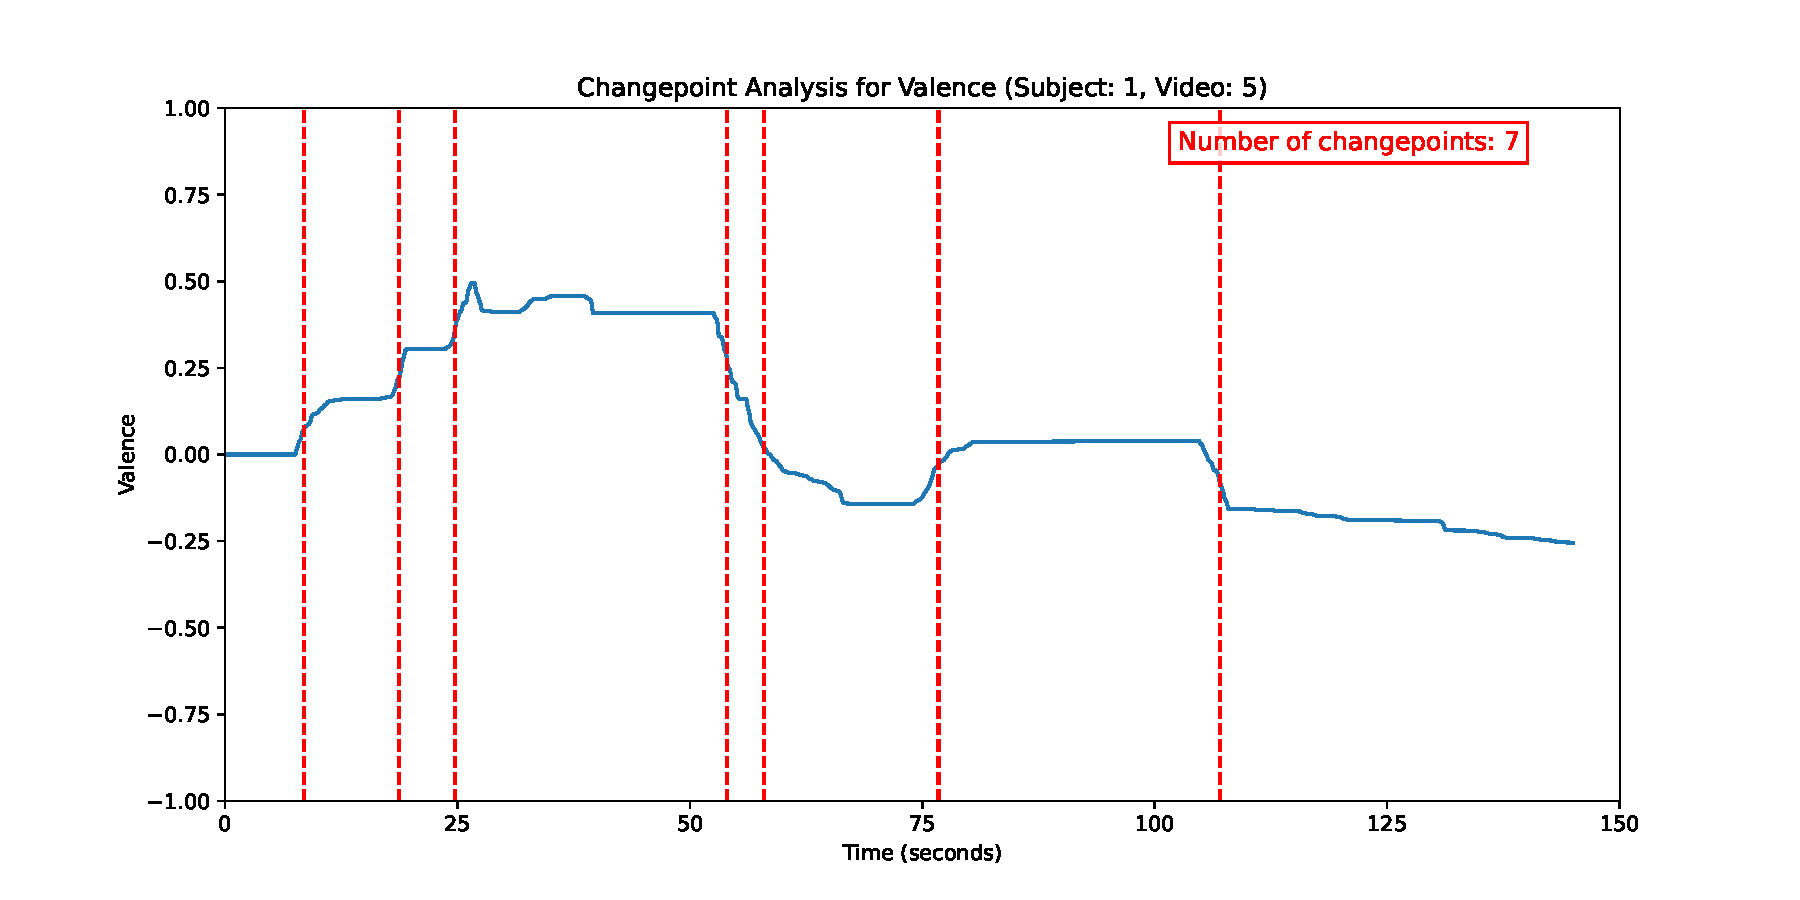
\includegraphics[width=\linewidth]{sub_1_changepoints_V5_valence} 
        \caption{} \label{fig:sub_1_changepoints_V5_valence}
    \end{subfigure}

    \vspace{1cm}
    
        \centering
    \begin{subfigure}[t]{0.49\textwidth}
        \centering
        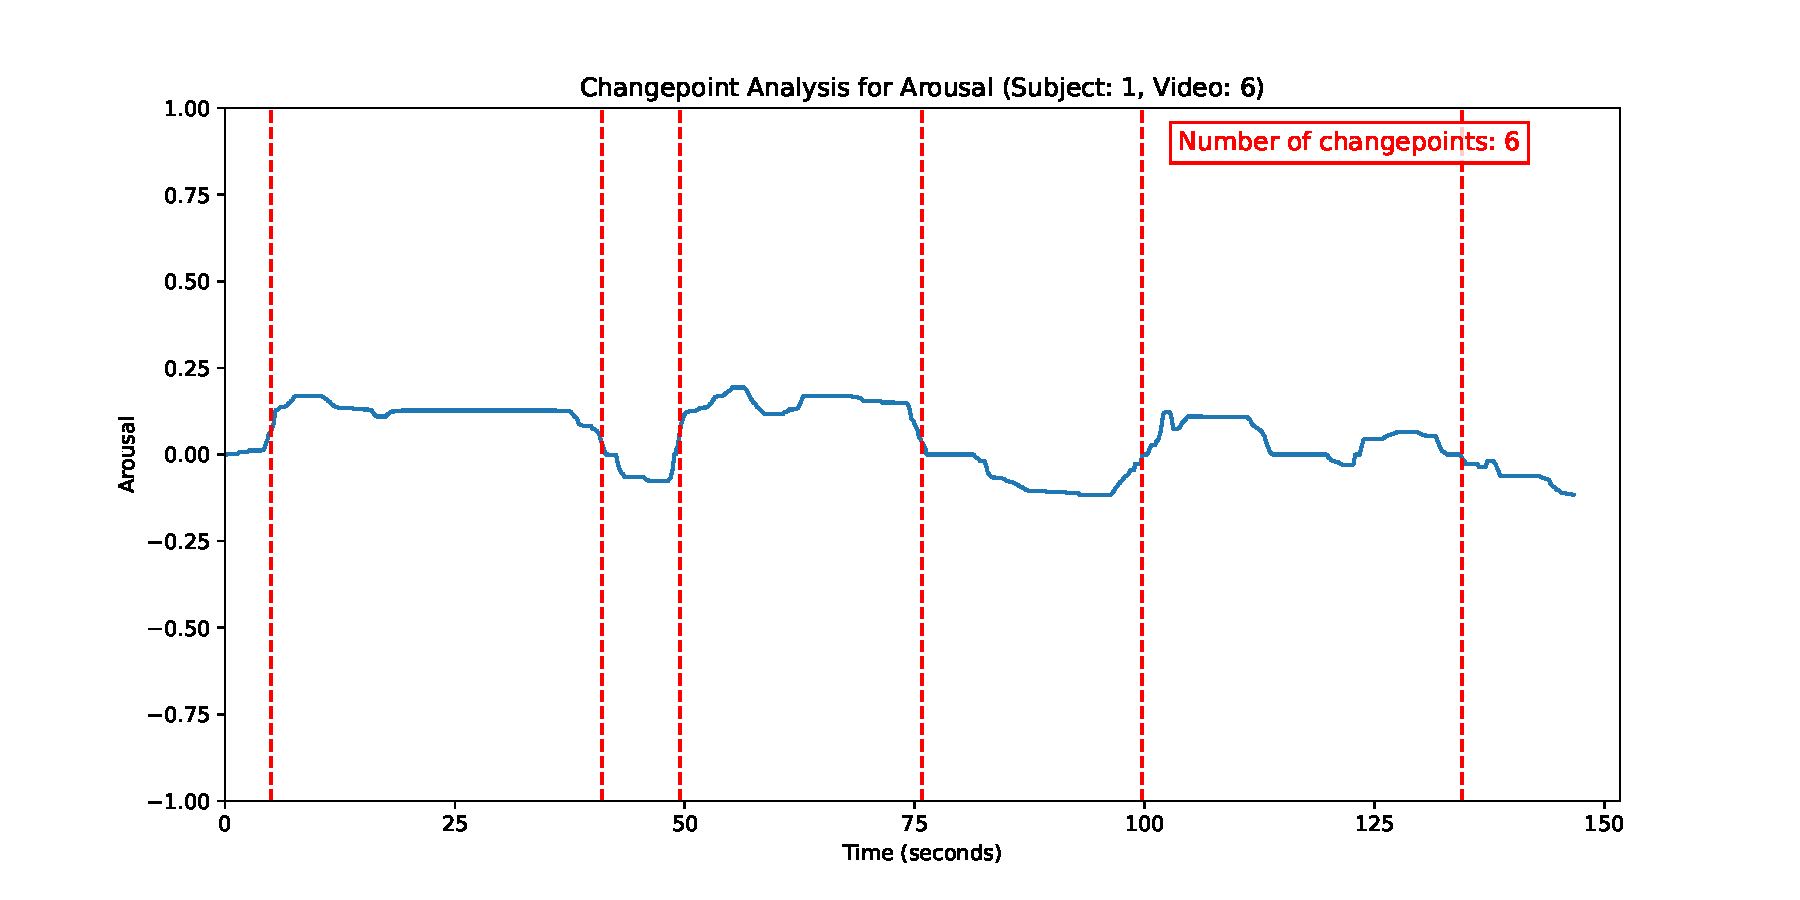
\includegraphics[width=\linewidth]{sub_1_changepoints_V6_arousal} 
        \caption{} \label{fig:sub_1_changepoints_V6_arousal}
    \end{subfigure}
    \hfill
    \begin{subfigure}[t]{0.49\textwidth}
        \centering
        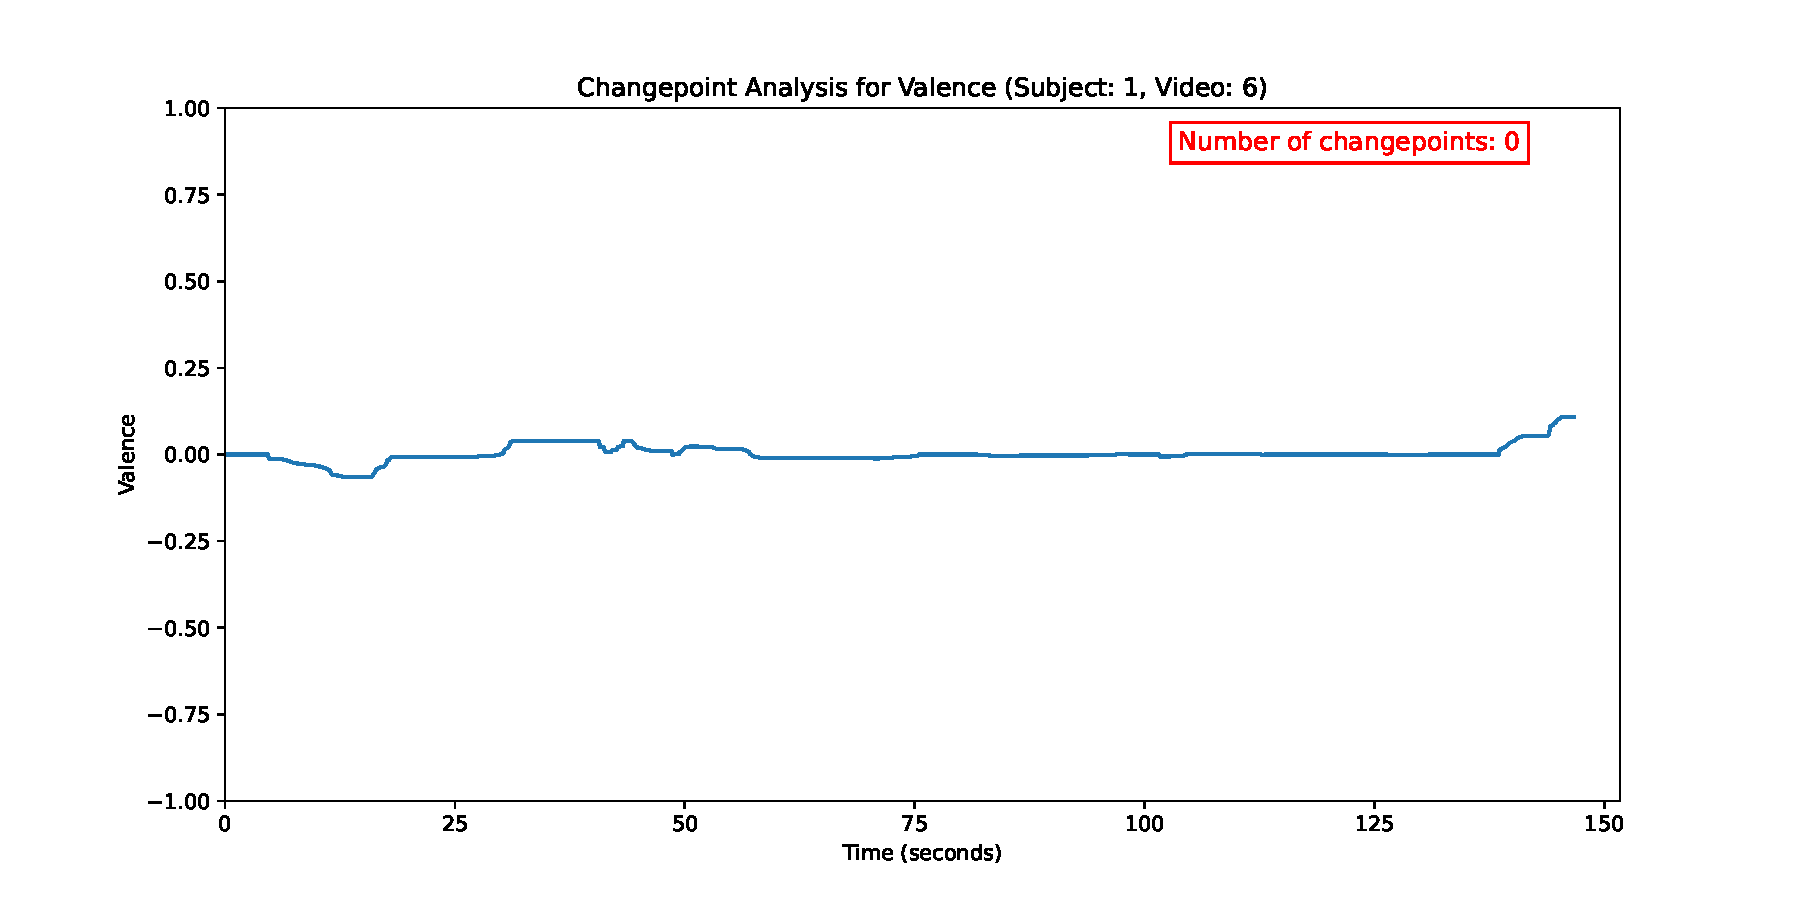
\includegraphics[width=\linewidth]{sub_1_changepoints_V6_valence} 
        \caption{} \label{fig:sub_1_changepoints_V6_valence}
    \end{subfigure}

    \vspace{1cm}
    
        \centering
    \begin{subfigure}[t]{0.49\textwidth}
        \centering
        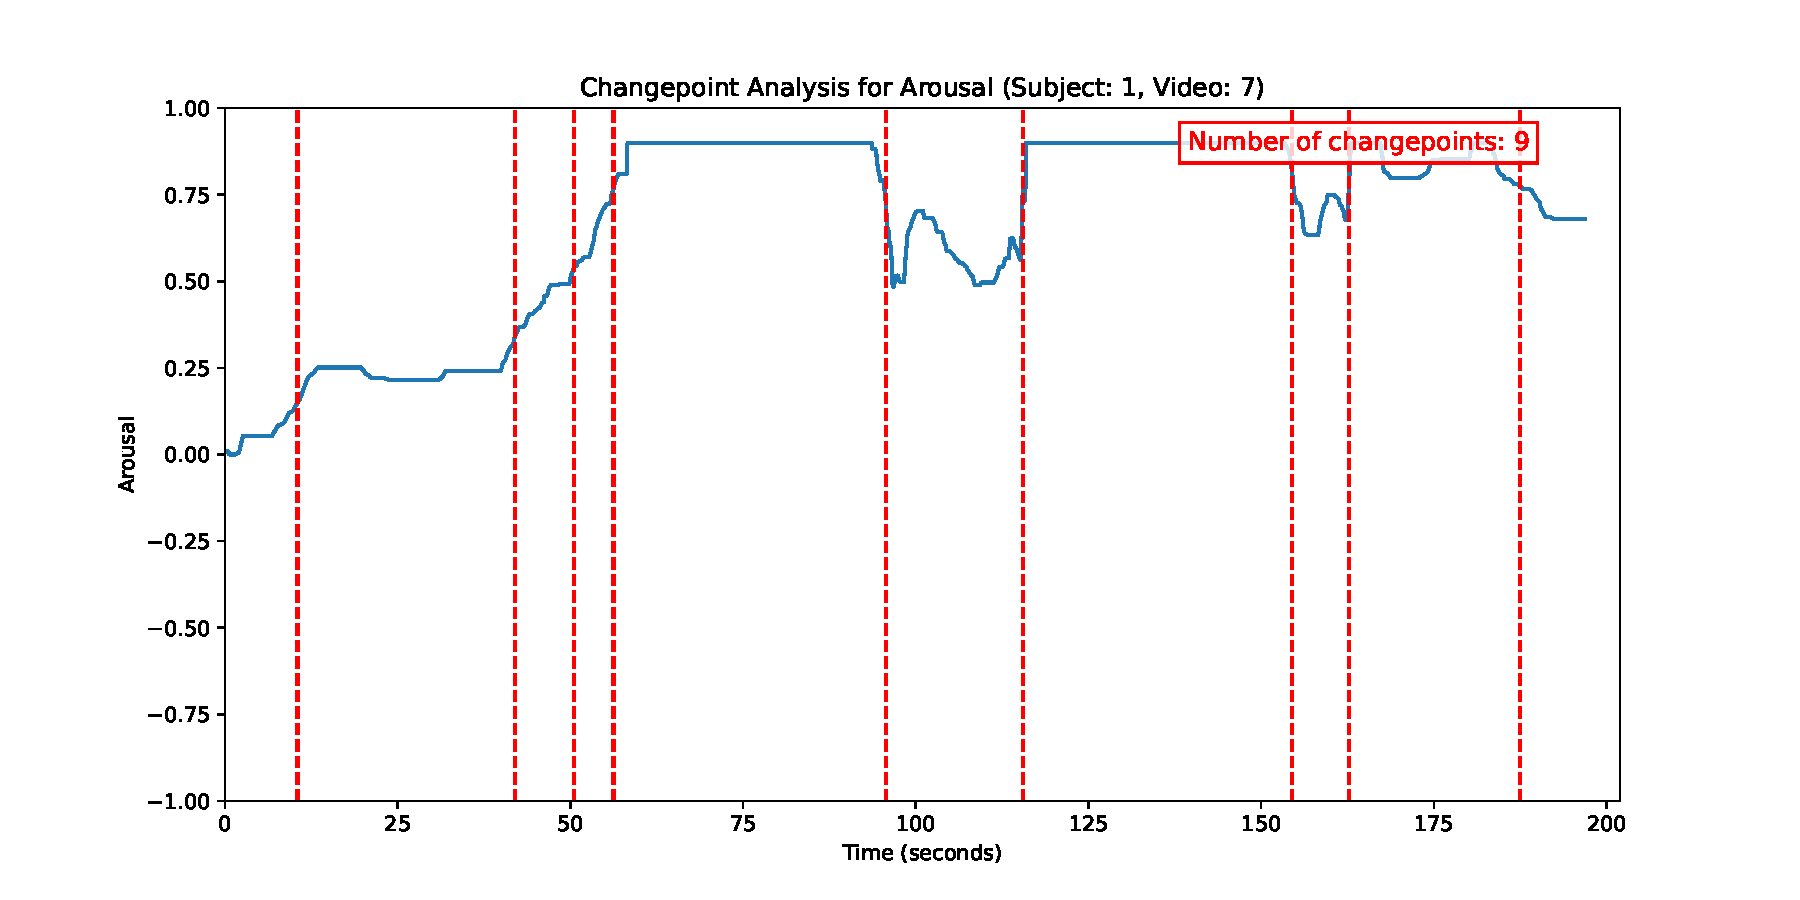
\includegraphics[width=\linewidth]{sub_1_changepoints_V7_arousal} 
        \caption{} \label{fig:sub_1_changepoints_V7_arousal}
    \end{subfigure}
    \hfill
    \begin{subfigure}[t]{0.49\textwidth}
        \centering
        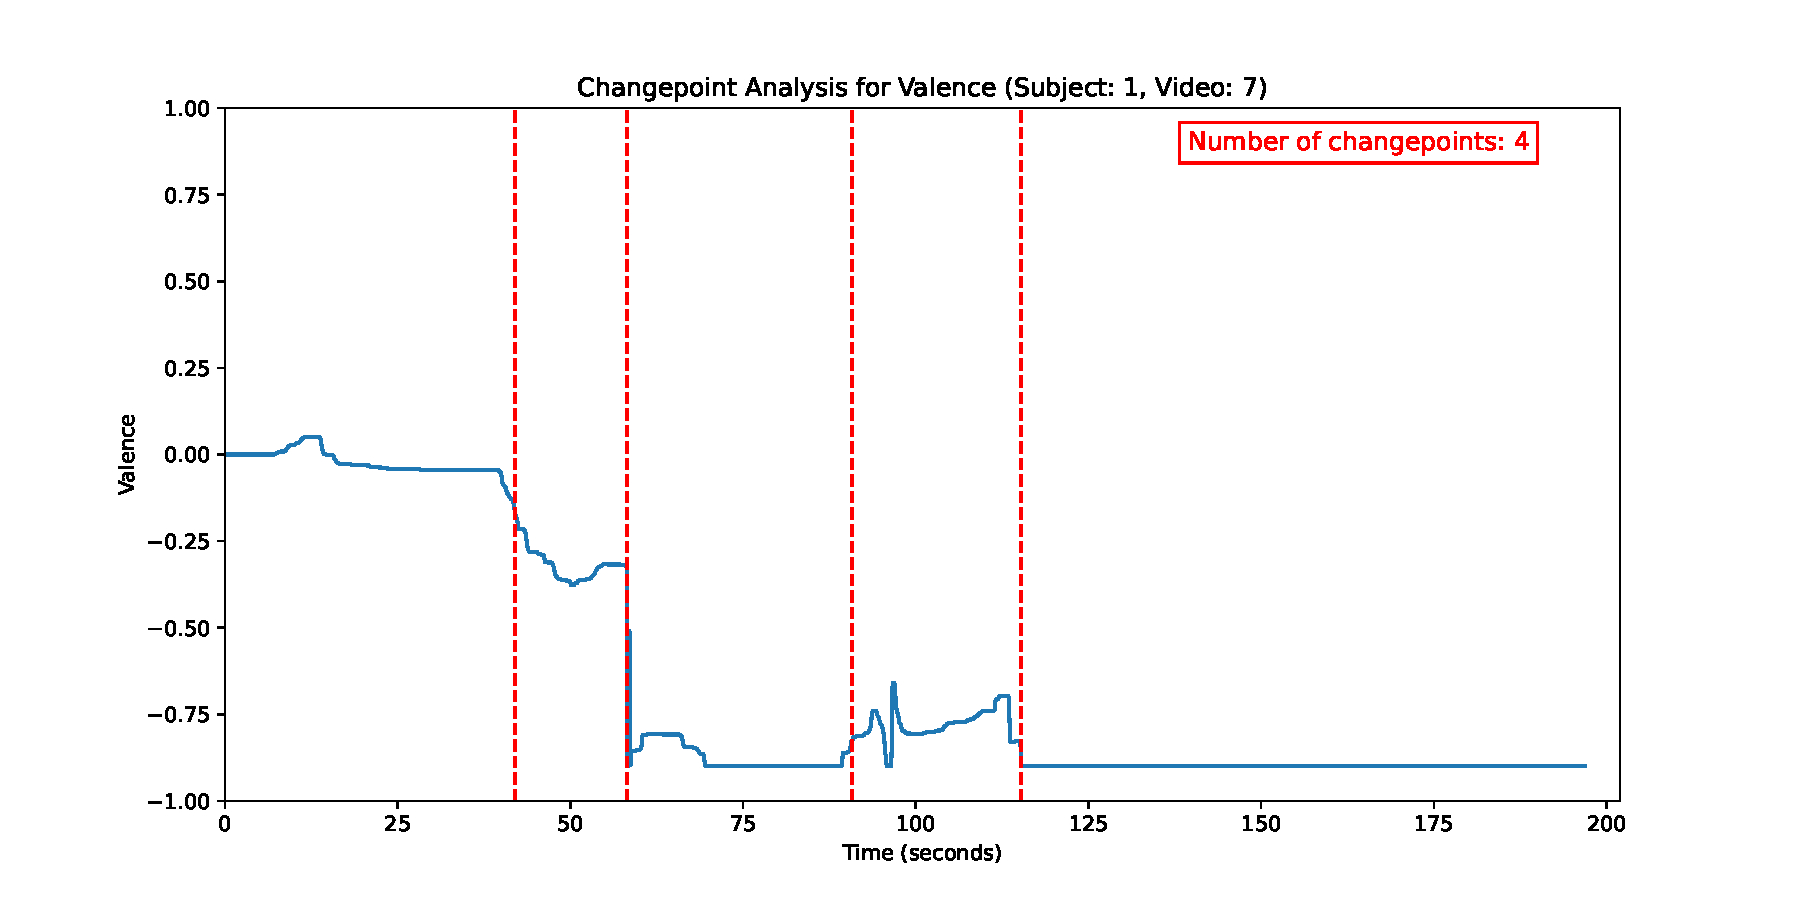
\includegraphics[width=\linewidth]{sub_1_changepoints_V7_valence} 
        \caption{} \label{fig:sub_1_changepoints_V7_valence}
    \end{subfigure}

    \vspace{1cm}
    
        \centering
    \begin{subfigure}[t]{0.49\textwidth}
        \centering
        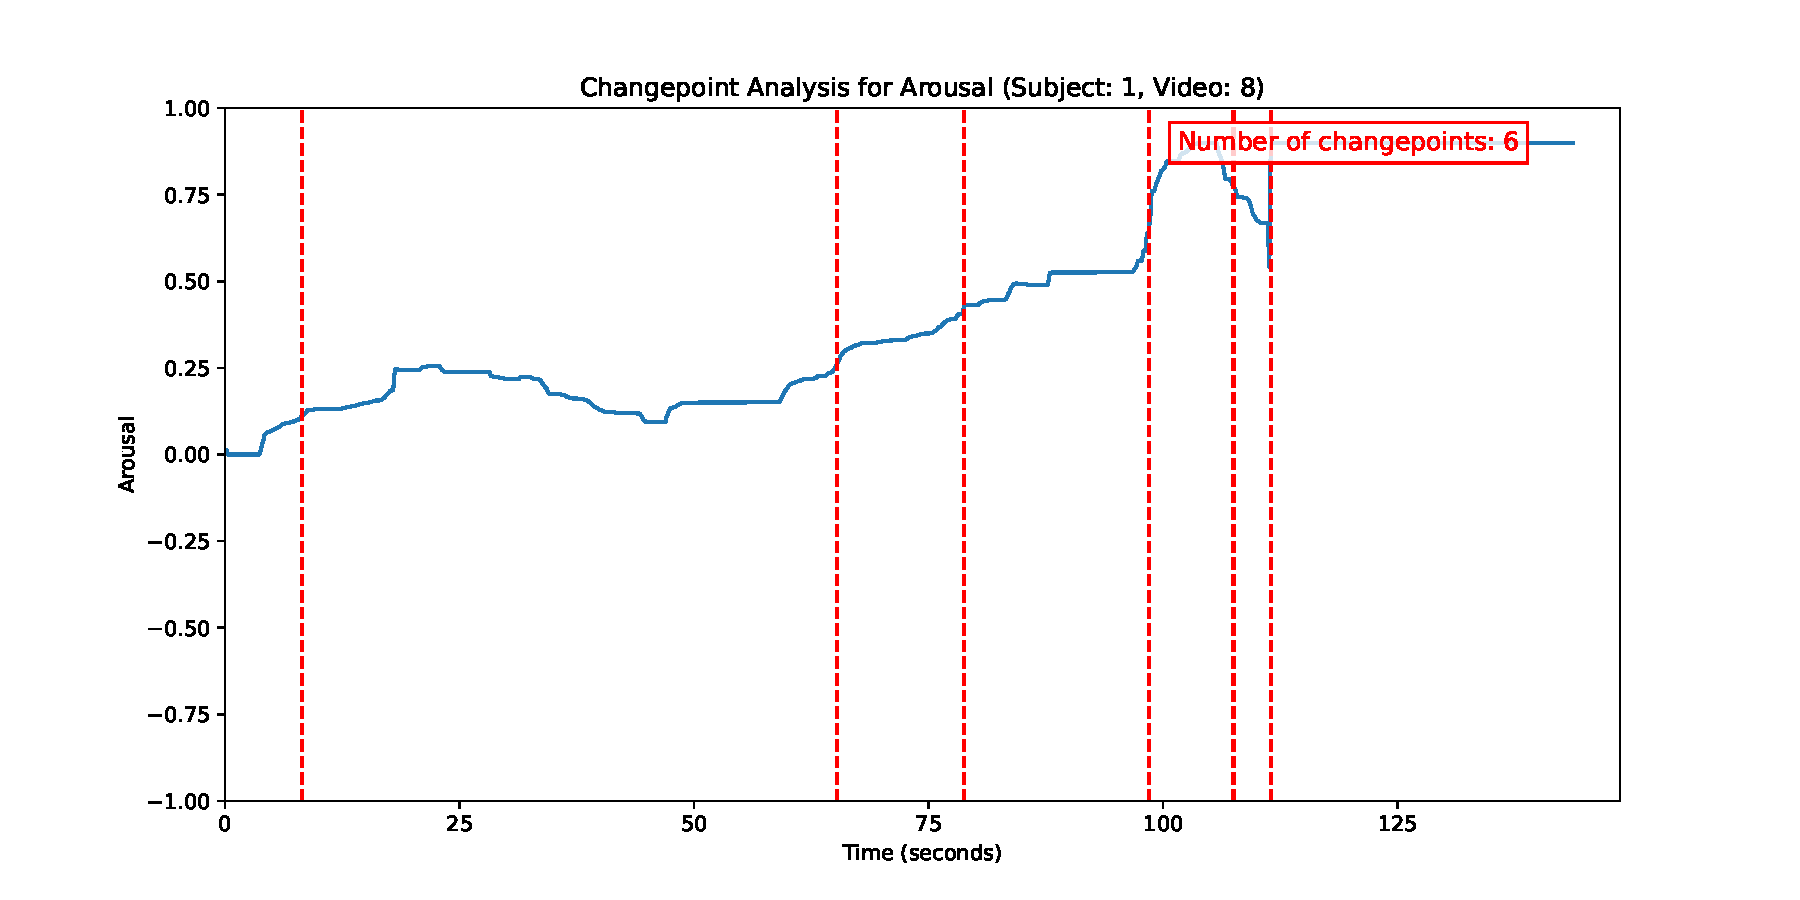
\includegraphics[width=\linewidth]{sub_1_changepoints_V8_arousal} 
        \caption{} \label{fig:sub_1_changepoints_V8_arousal}
    \end{subfigure}
    \hfill
    \begin{subfigure}[t]{0.49\textwidth}
        \centering
        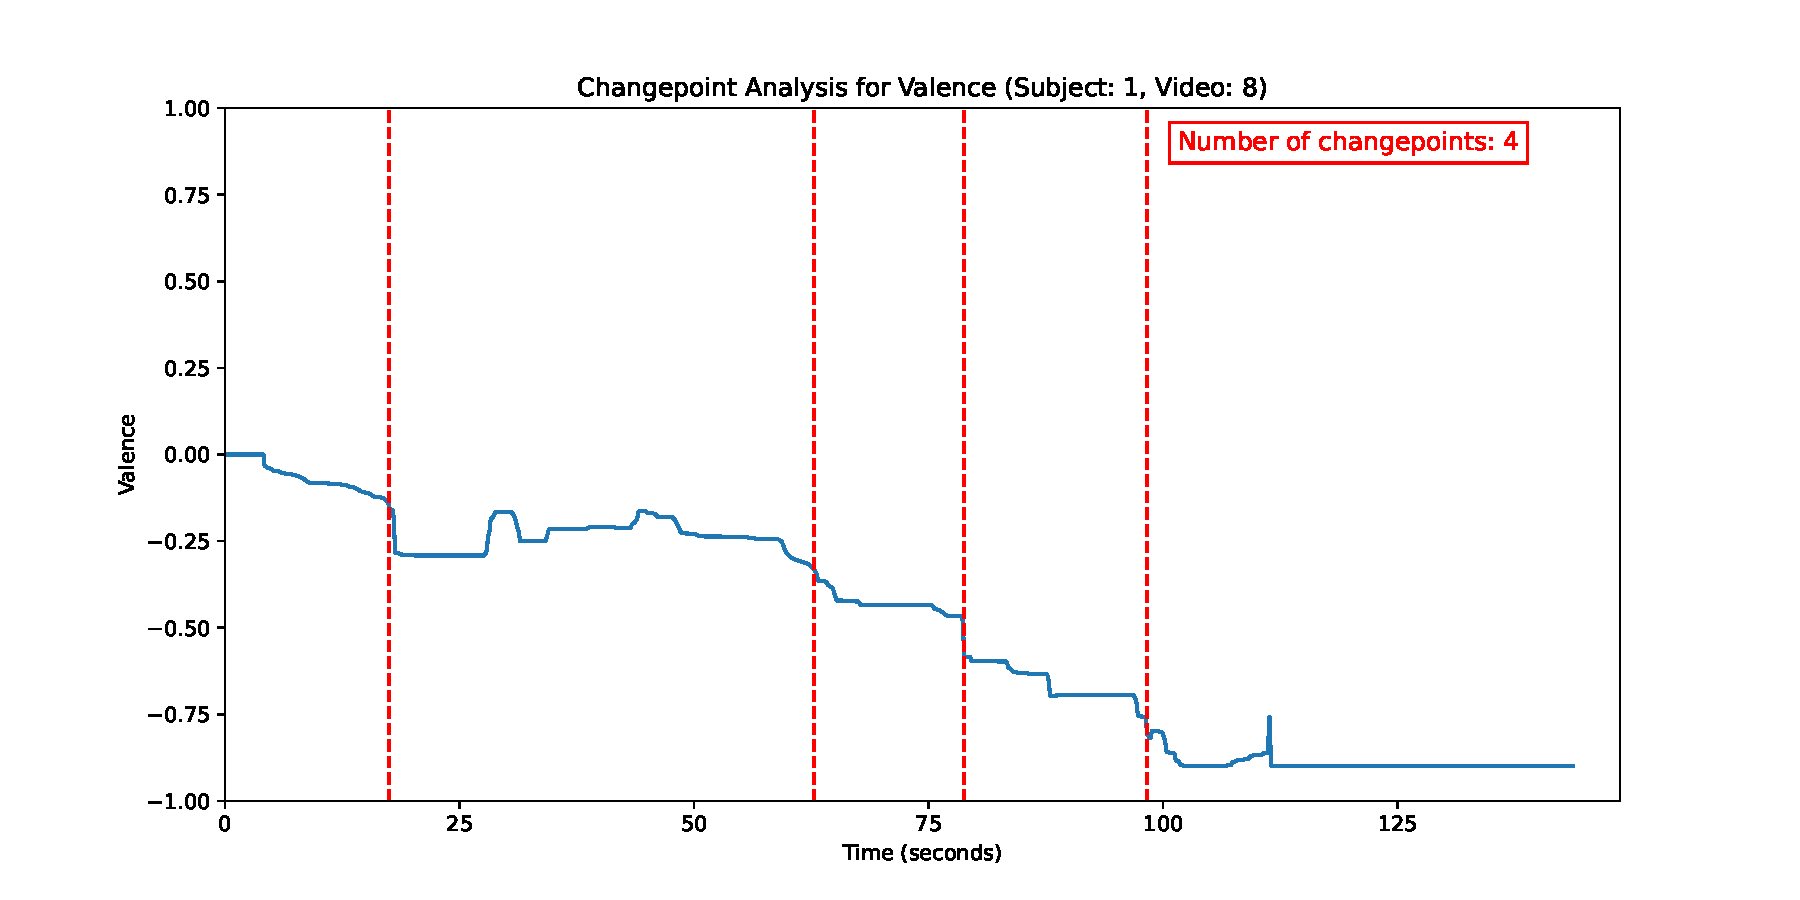
\includegraphics[width=\linewidth]{sub_1_changepoints_V8_valence} 
        \caption{} \label{fig:sub_1_changepoints_V8_valence}
    \end{subfigure}

    \vspace{1cm}
    
    \caption{\textit{Change points in arousal and valence ratings for all videos for one subject.} Change points as identified by the algorithm for each video's arousal (left column) and valence (right column) ratings for subject 1. Red dashed lines indicate the change points, the thin blue line is the subject's continuous rating. The number of change points identified is given in the top right corner of each plot. Note the different lengths of the videos.}
    \label{fig:sub1}
\end{figure}

\newpage

% +++++ subsection cpa averaged across participants ++++++
\subsection{CPA for data averaged across participants}
Figure \ref{fig:all_data} shows the shows the change points identified for each video's arousal and valence ratings averaged across subjects. Additionally, all subjects' annotation timeseries for valence and arousal are depicted to show the interindividual differences in ratings. Even though the algorithm seems to be able to identify change points in all videos, only video 7 and video 8 seemed to have significant changes in valence and arousal ratings. As those were the two videos labelled as 'scary' by the authors, it seems plausible that participants' rating varied more in these videos and were more extreme than in the other videos. For the other two high arousing but positive videos (1 and 2), more change points have been identified than in the low arousing videos, albeit this effect is less than in the negative videos. Note the high differences between individual participants in their emotion ratings.
See table \ref{tab:table_avg_cpa} for the x-coordinates (timestamps) of the averaged change points for all videos and for both arousal and valence.

% figure cpa all data
\begin{figure}
    \centering
    \begin{subfigure}[t]{0.49\textwidth}
        \centering
        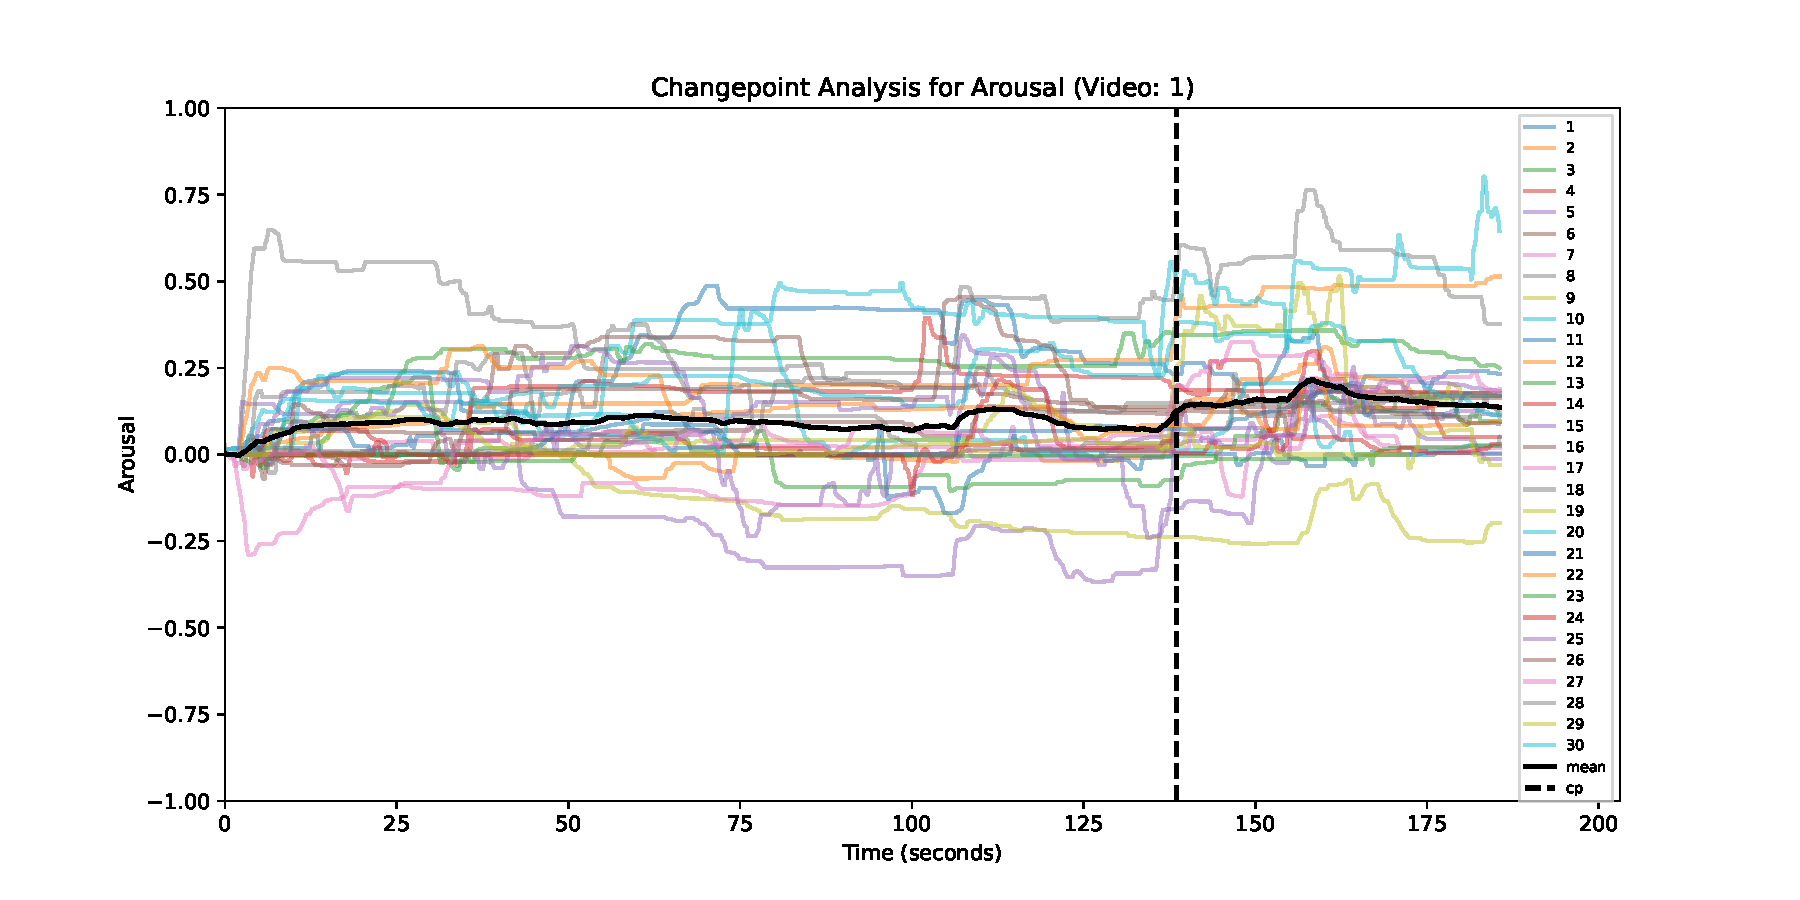
\includegraphics[width=\linewidth]{changepoints_V1_arousal_avg_all_data} 
        \caption{} \label{fig:changepoints_V1_arousal_avg_all_data}
    \end{subfigure}
    \hfill
    \begin{subfigure}[t]{0.49\textwidth}
        \centering
        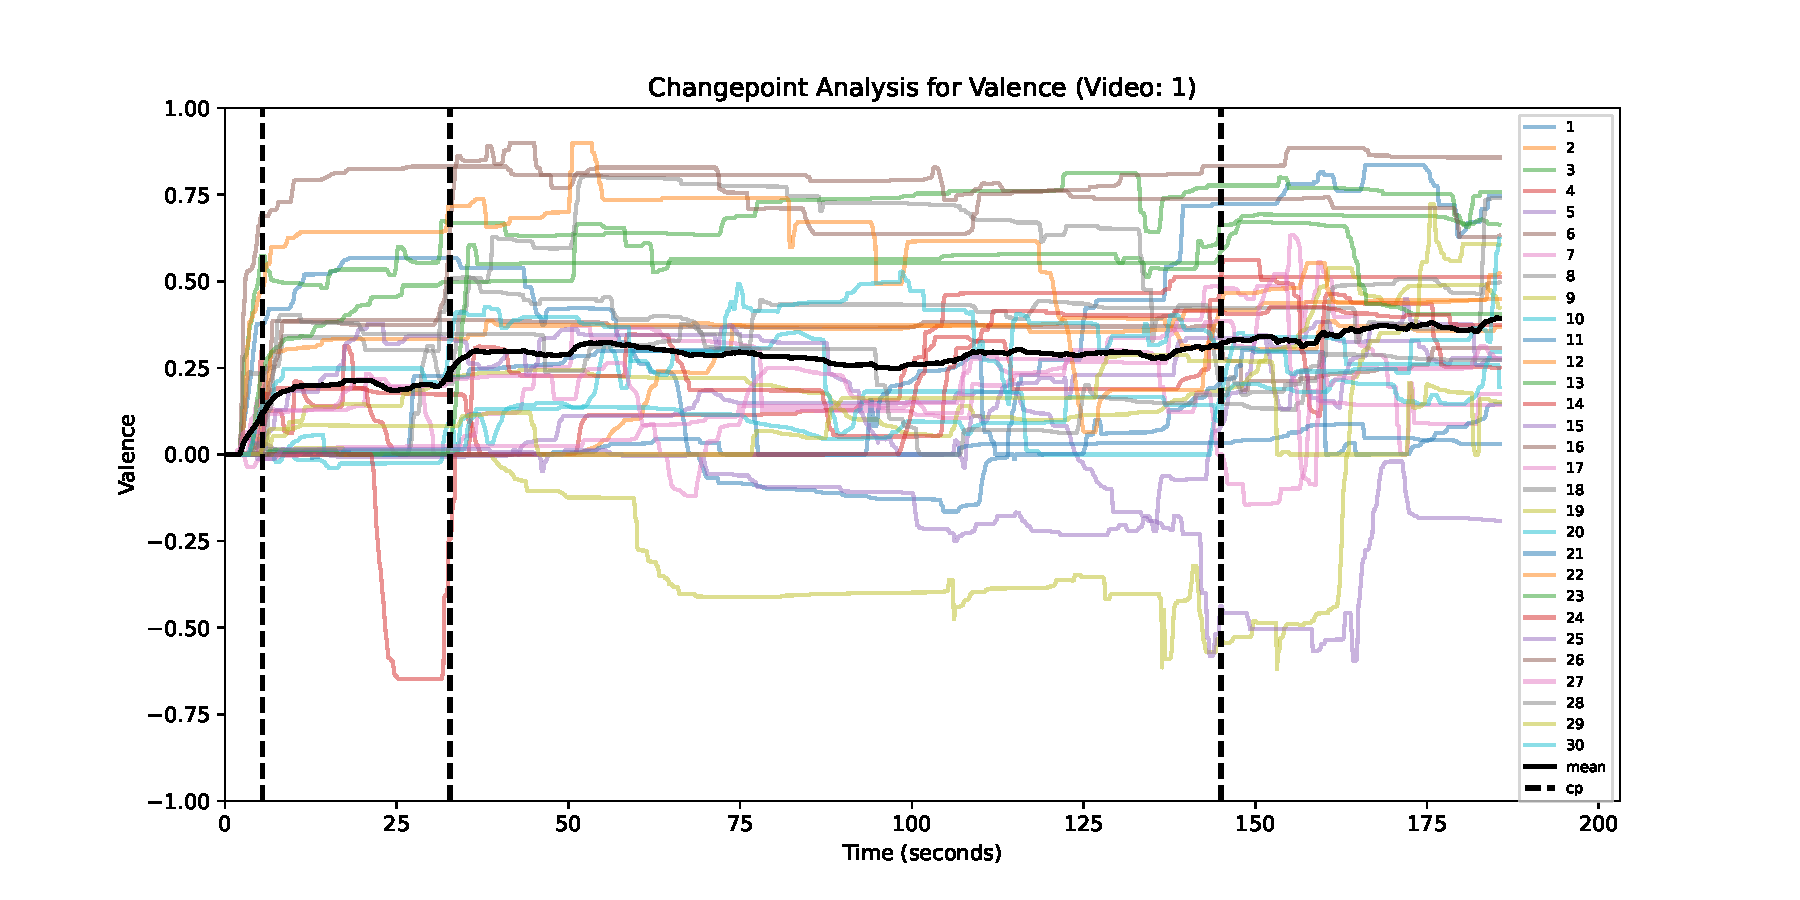
\includegraphics[width=\linewidth]{changepoints_V1_valence_avg_all_data} 
        \caption{} \label{fig:changepoints_V1_valence_avg_all_data}
    \end{subfigure}

    \vspace{1cm}
    
    \centering
    \begin{subfigure}[t]{0.49\textwidth}
        \centering
        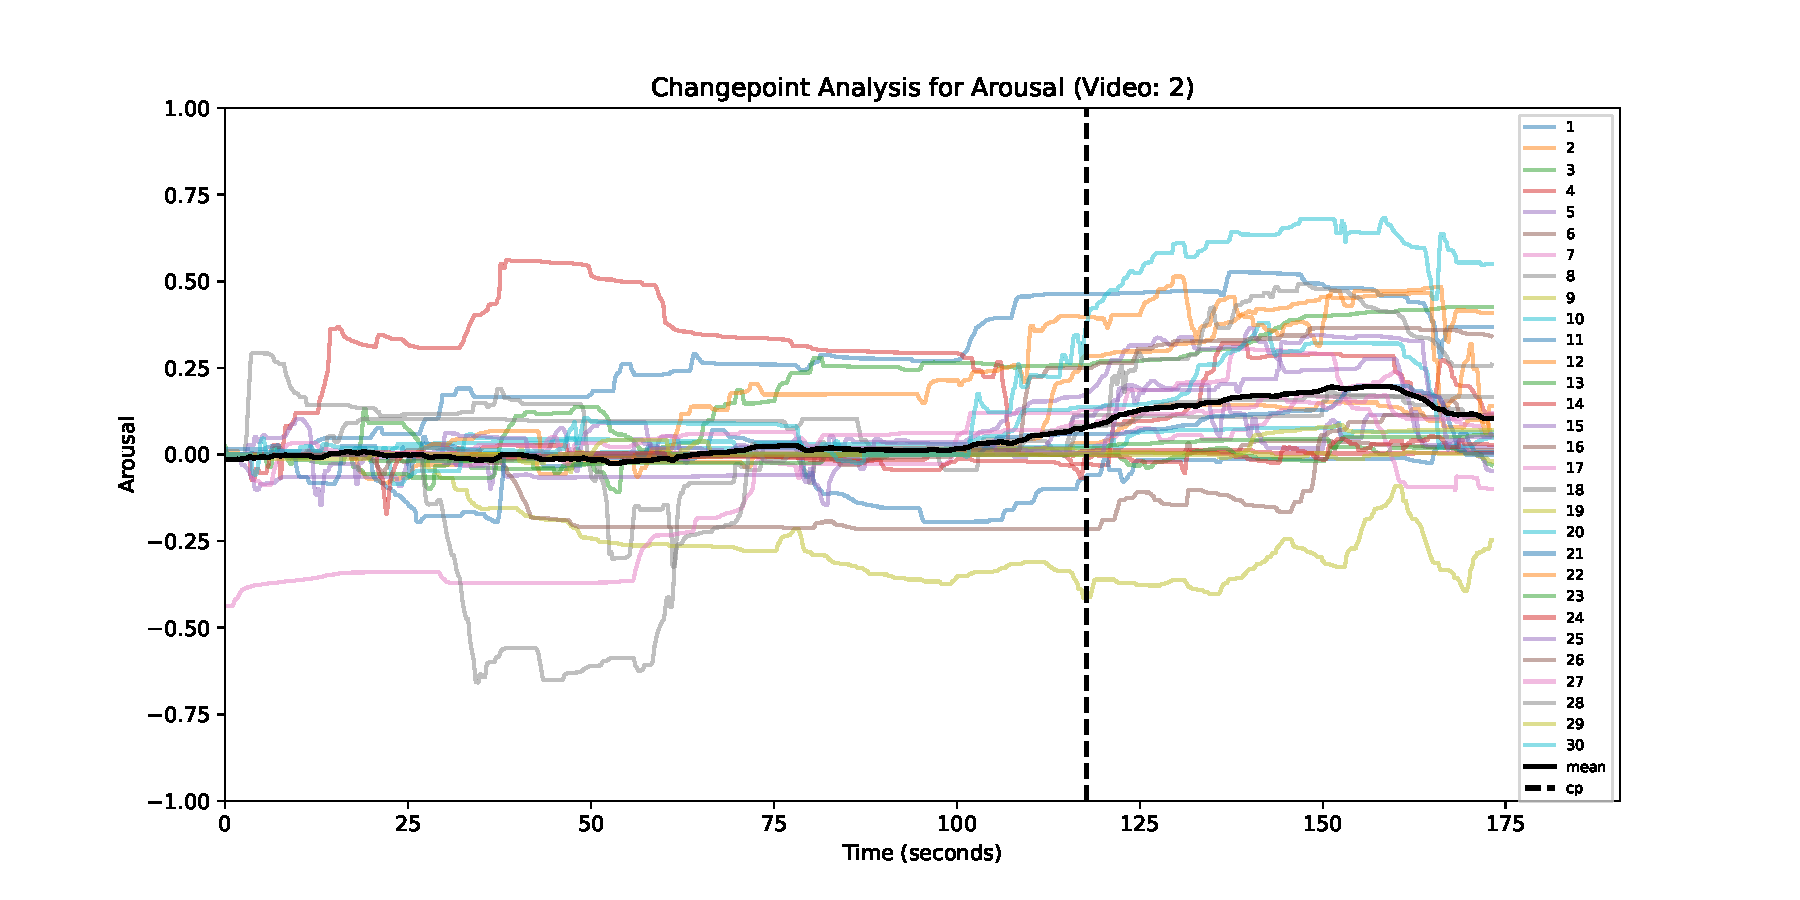
\includegraphics[width=\linewidth]{changepoints_V2_arousal_avg_all_data} 
        \caption{} \label{fig:changepoints_V2_arousal_avg_all_data}
    \end{subfigure}
    \hfill
    \begin{subfigure}[t]{0.49\textwidth}
        \centering
        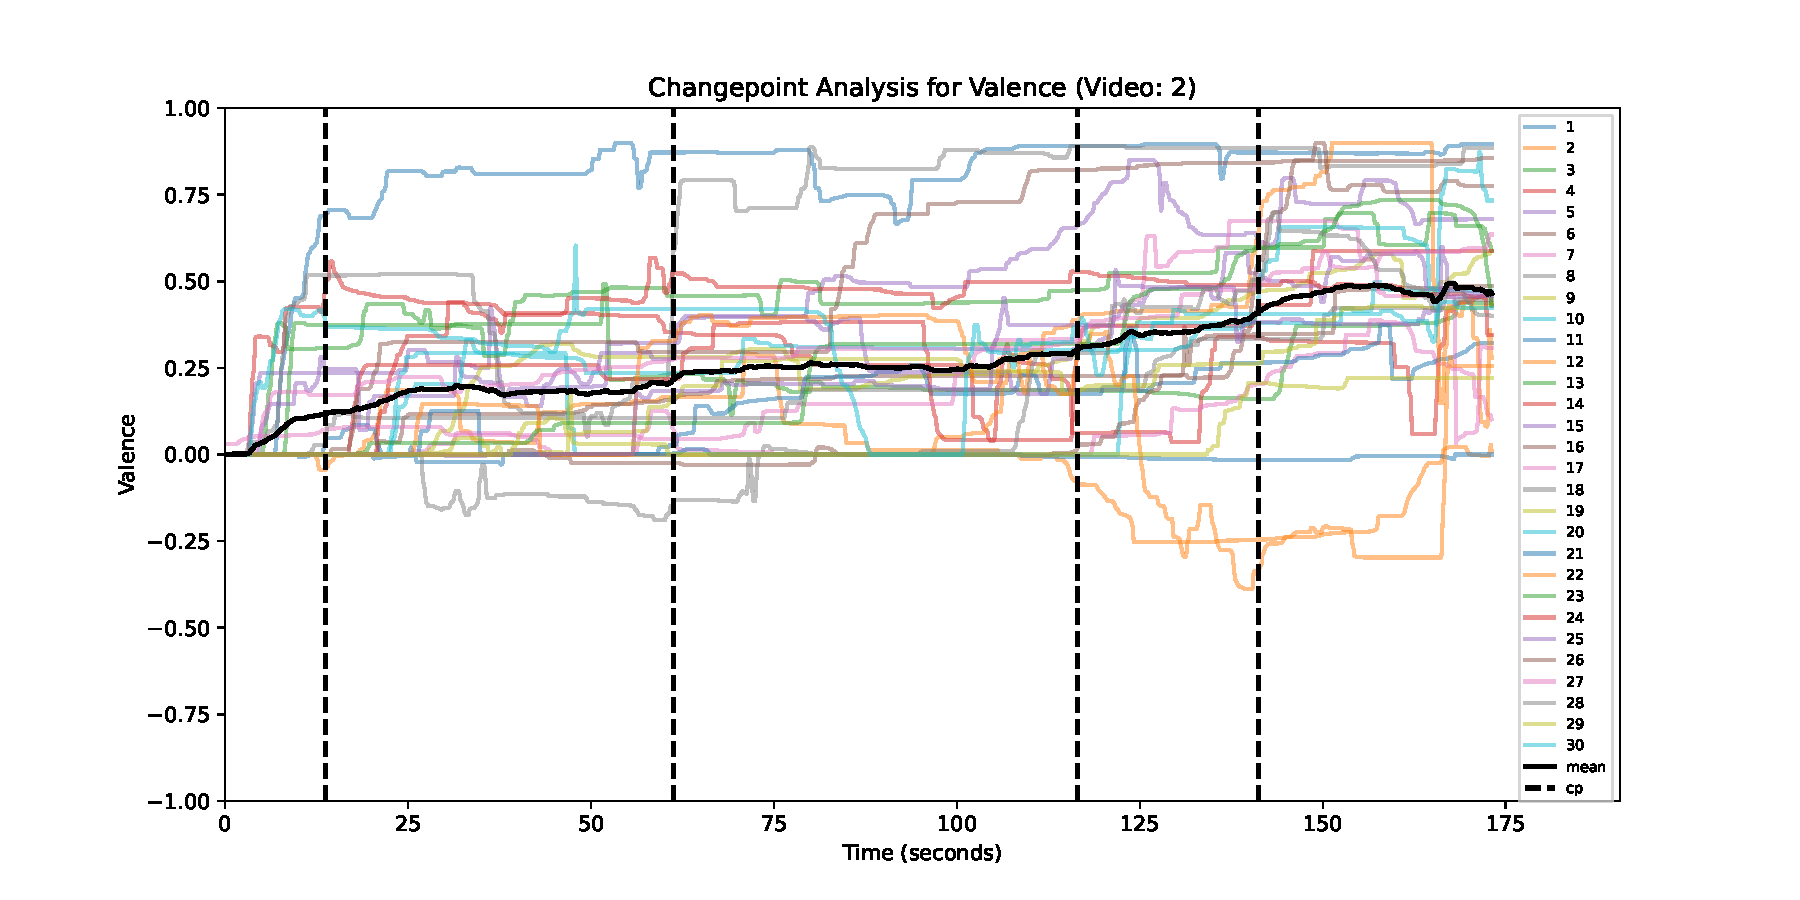
\includegraphics[width=\linewidth]{changepoints_V2_valence_avg_all_data} 
        \caption{} \label{fig:changepoints_V2_valence_avg_all_data}
    \end{subfigure}
    
        \centering
    \begin{subfigure}[t]{0.49\textwidth}
        \centering
        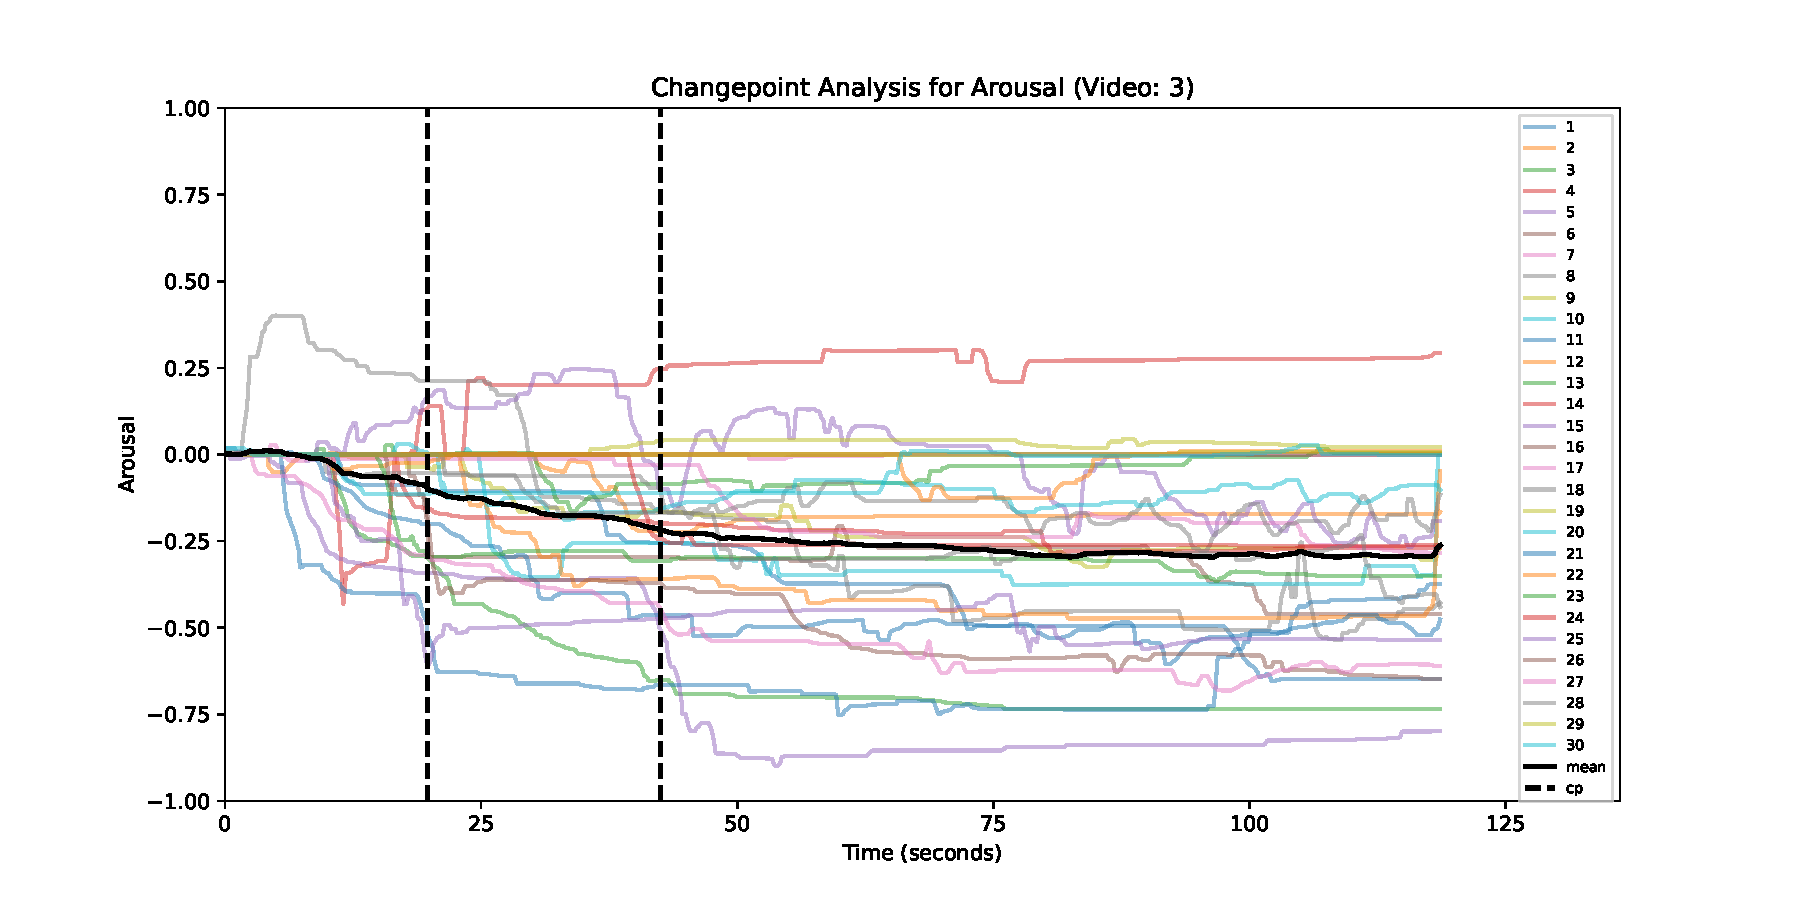
\includegraphics[width=\linewidth]{changepoints_V3_arousal_avg_all_data} 
        \caption{} \label{fig:changepoints_V3_arousal_avg_all_data}
    \end{subfigure}
    \hfill
    \begin{subfigure}[t]{0.49\textwidth}
        \centering
        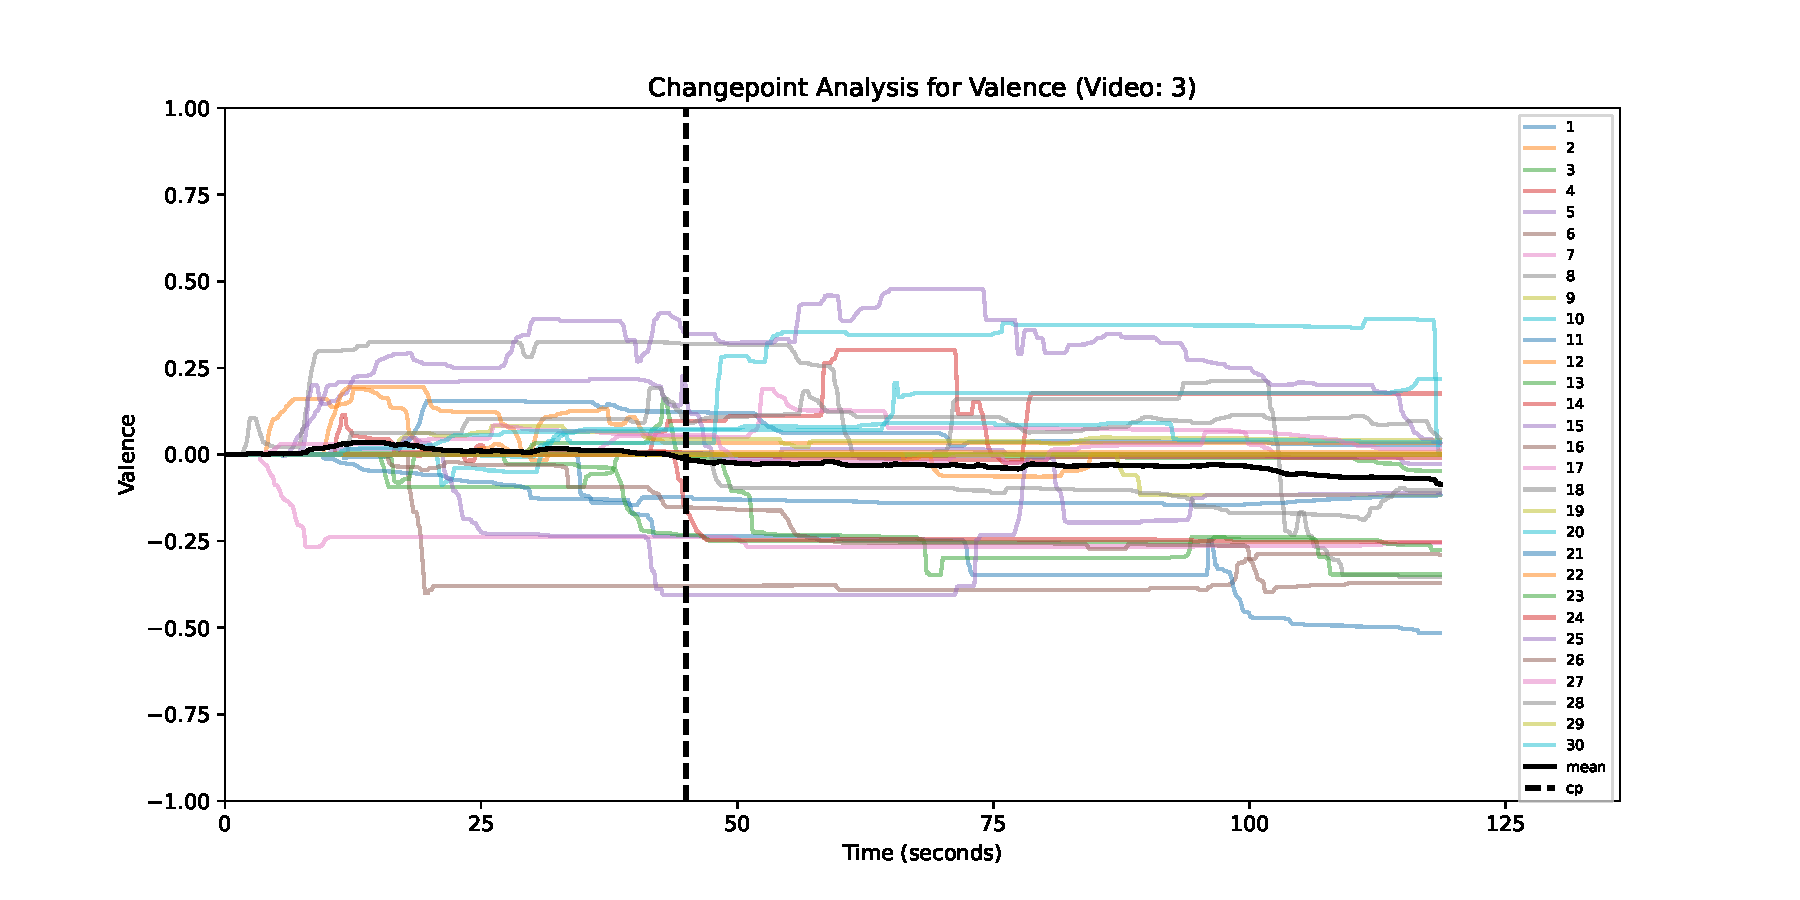
\includegraphics[width=\linewidth]{changepoints_V3_valence_avg_all_data} 
        \caption{} \label{fig:changepoints_V3_valence_avg_all_data}
    \end{subfigure}

    \vspace{1cm}
    
        \centering
    \begin{subfigure}[t]{0.49\textwidth}
        \centering
        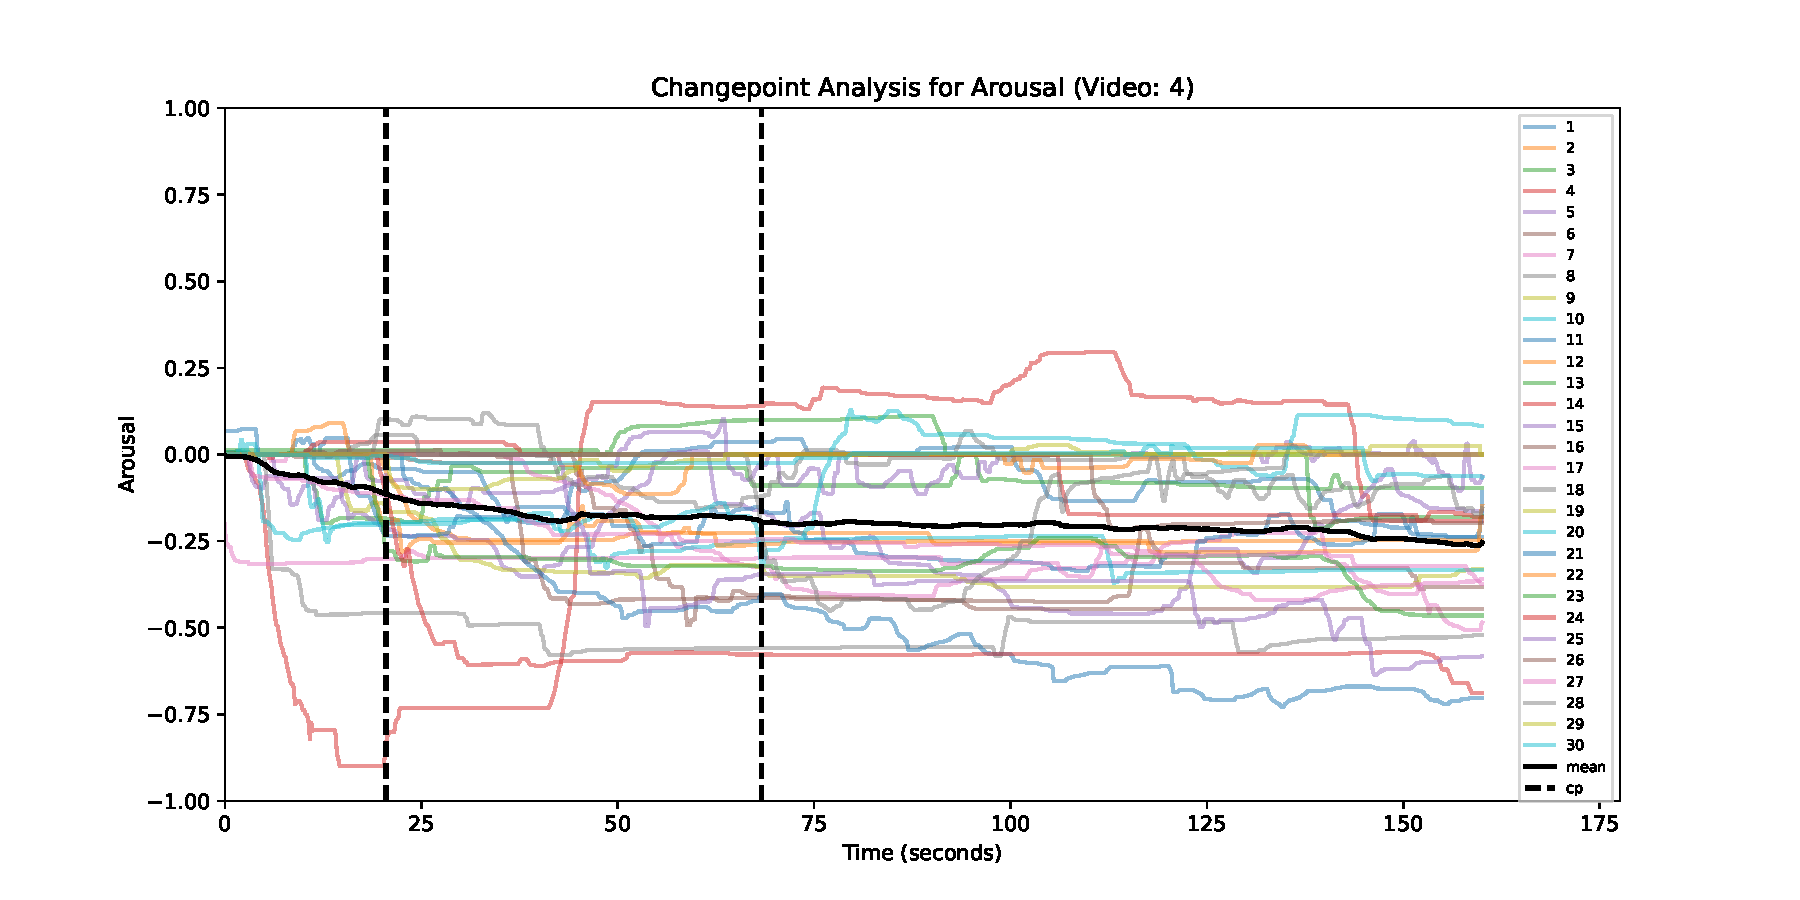
\includegraphics[width=\linewidth]{changepoints_V4_arousal_avg_all_data} 
        \caption{} \label{fig:changepoints_V4_arousal_avg_all_datal}
    \end{subfigure}
    \hfill
    \begin{subfigure}[t]{0.49\textwidth}
        \centering
        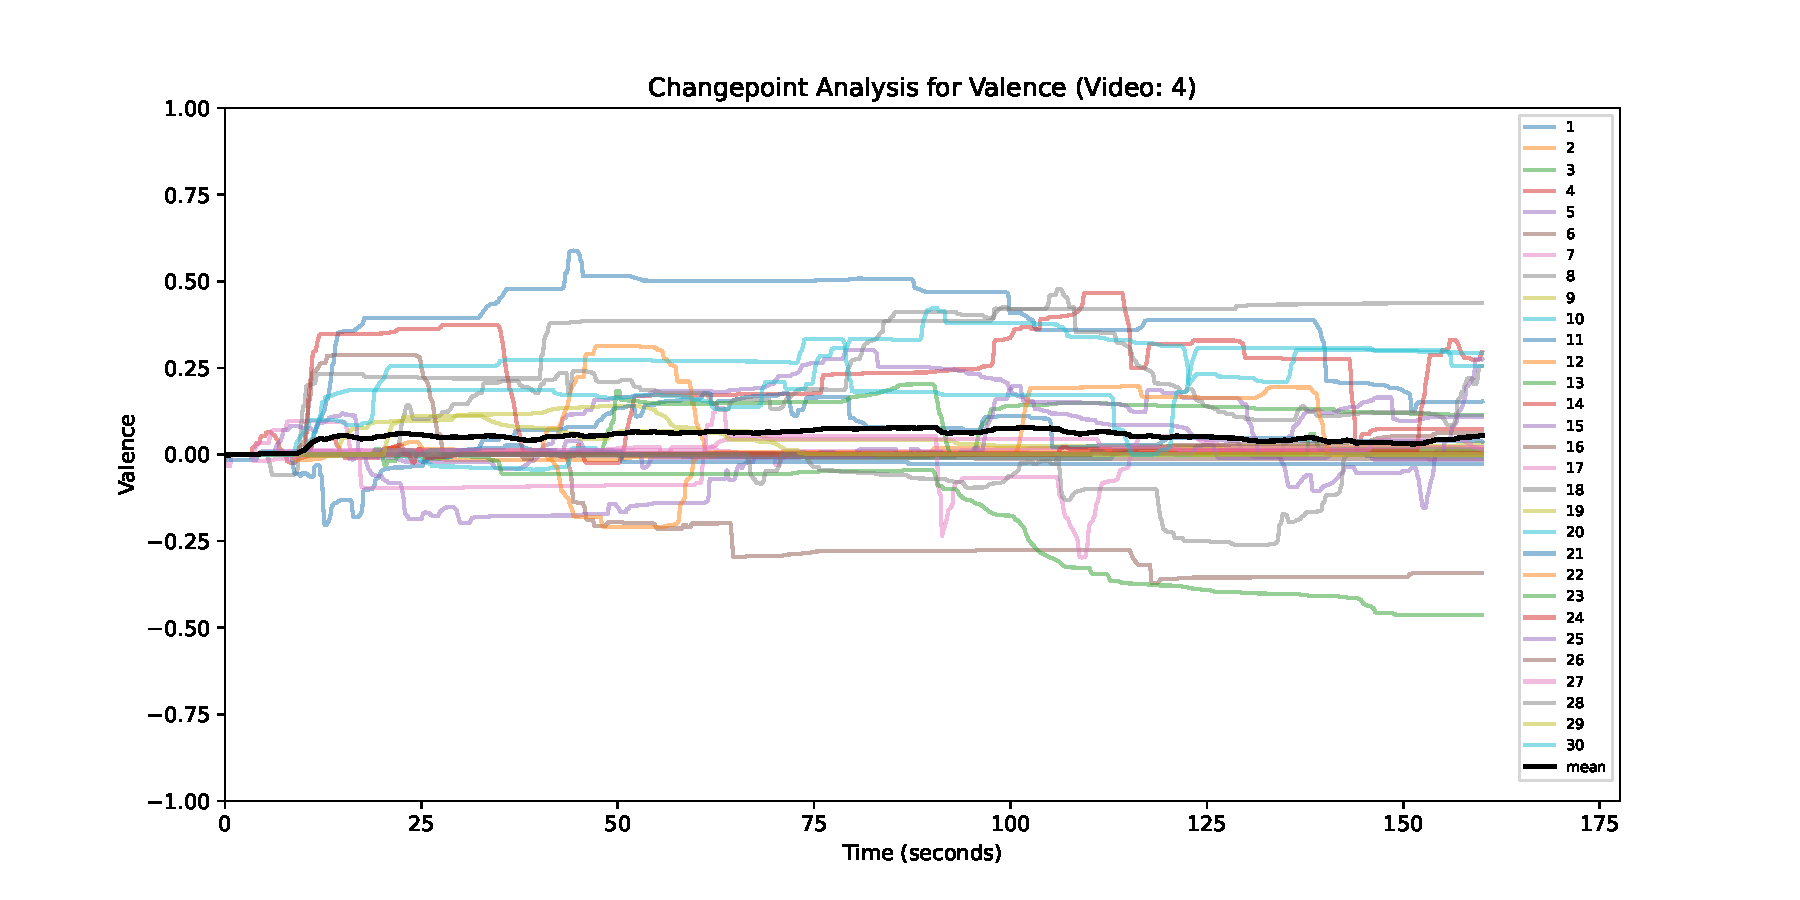
\includegraphics[width=\linewidth]{changepoints_V4_valence_avg_all_data} 
        \caption{} \label{fig:changepoints_V4_valence_avg_all_data}
    \end{subfigure}
 \end{figure}

 \begin{figure} \ContinuedFloat
        \centering
    \begin{subfigure}[t]{0.49\textwidth}
        \centering
        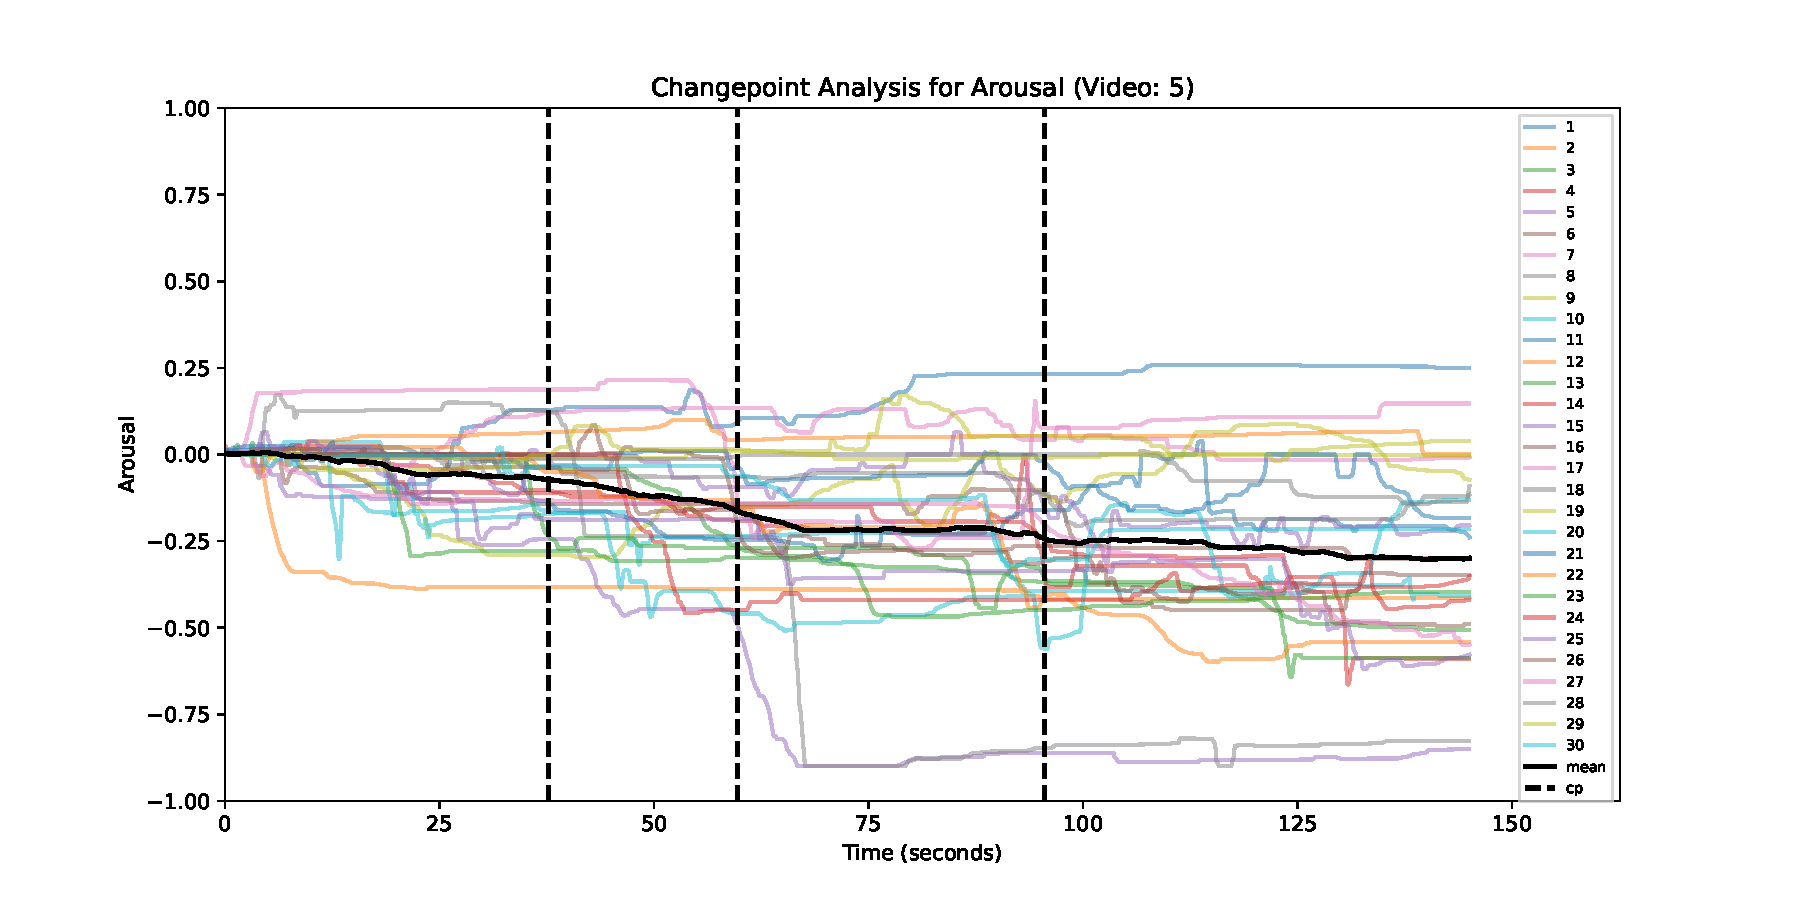
\includegraphics[width=\linewidth]{changepoints_V5_arousal_avg_all_data}
        \caption{} \label{fig:changepoints_V5_arousal_avg_all_data}
    \end{subfigure}
    \hfill
    \begin{subfigure}[t]{0.49\textwidth}
        \centering
        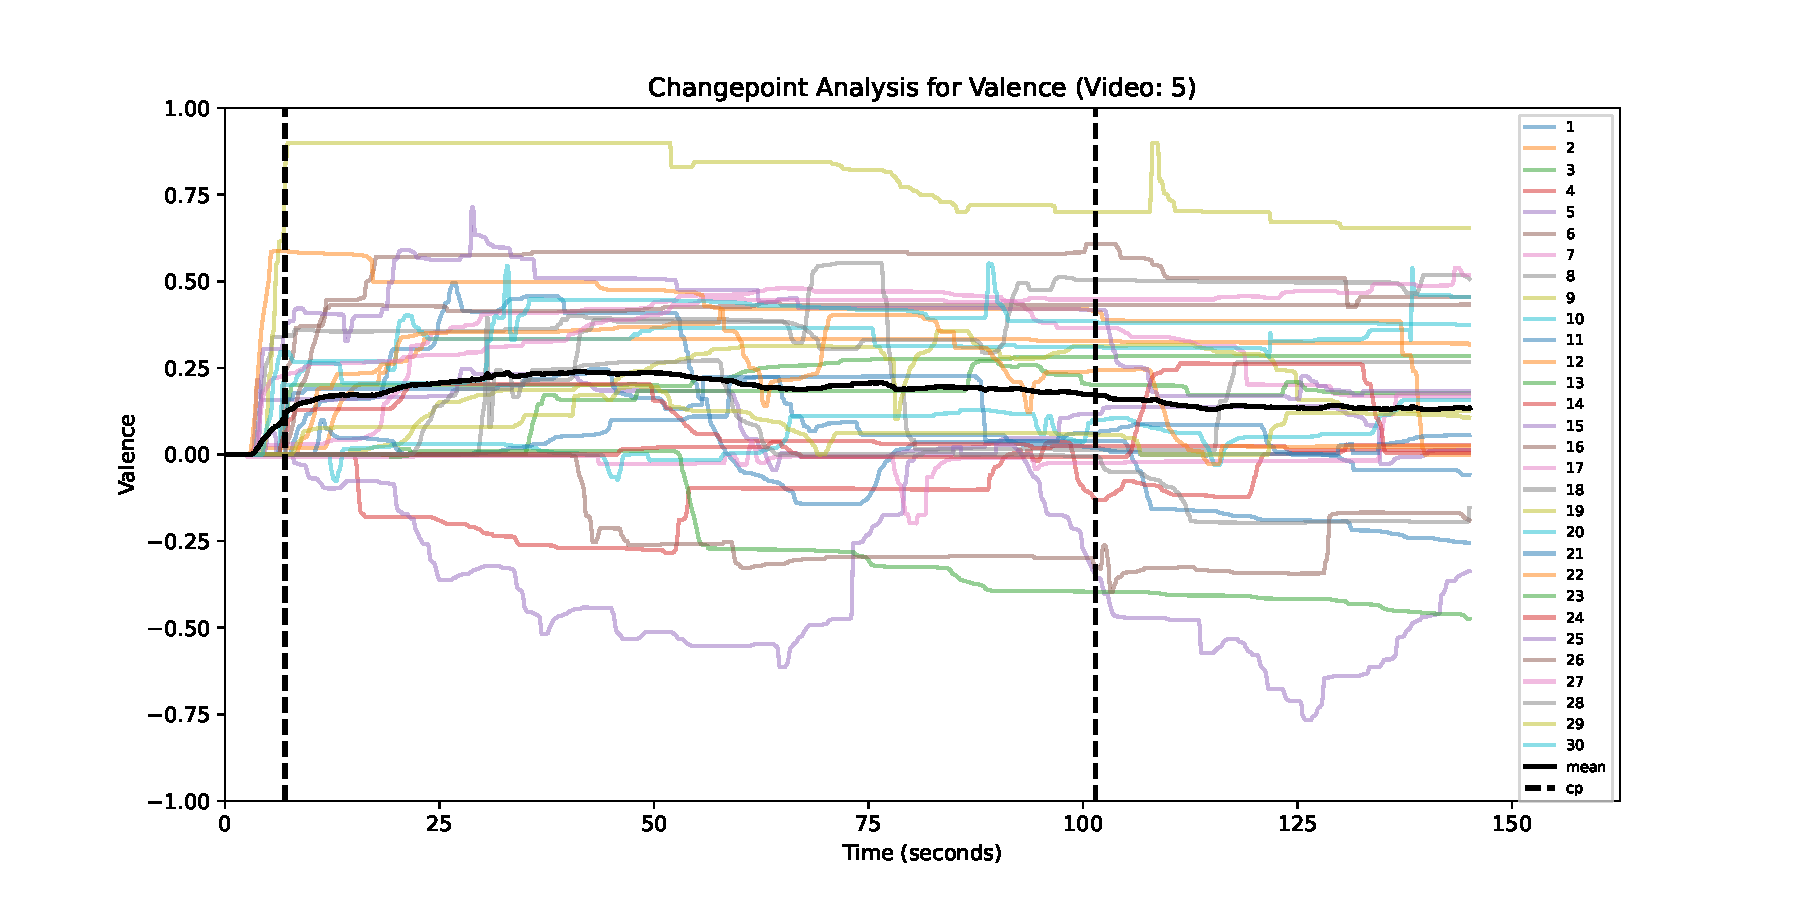
\includegraphics[width=\linewidth]{changepoints_V5_valence_avg_all_data} 
        \caption{} \label{fig:changepoints_V5_valence_avg_all_data}
    \end{subfigure}

    \vspace{1cm}
    
        \centering
    \begin{subfigure}[t]{0.49\textwidth}
        \centering
        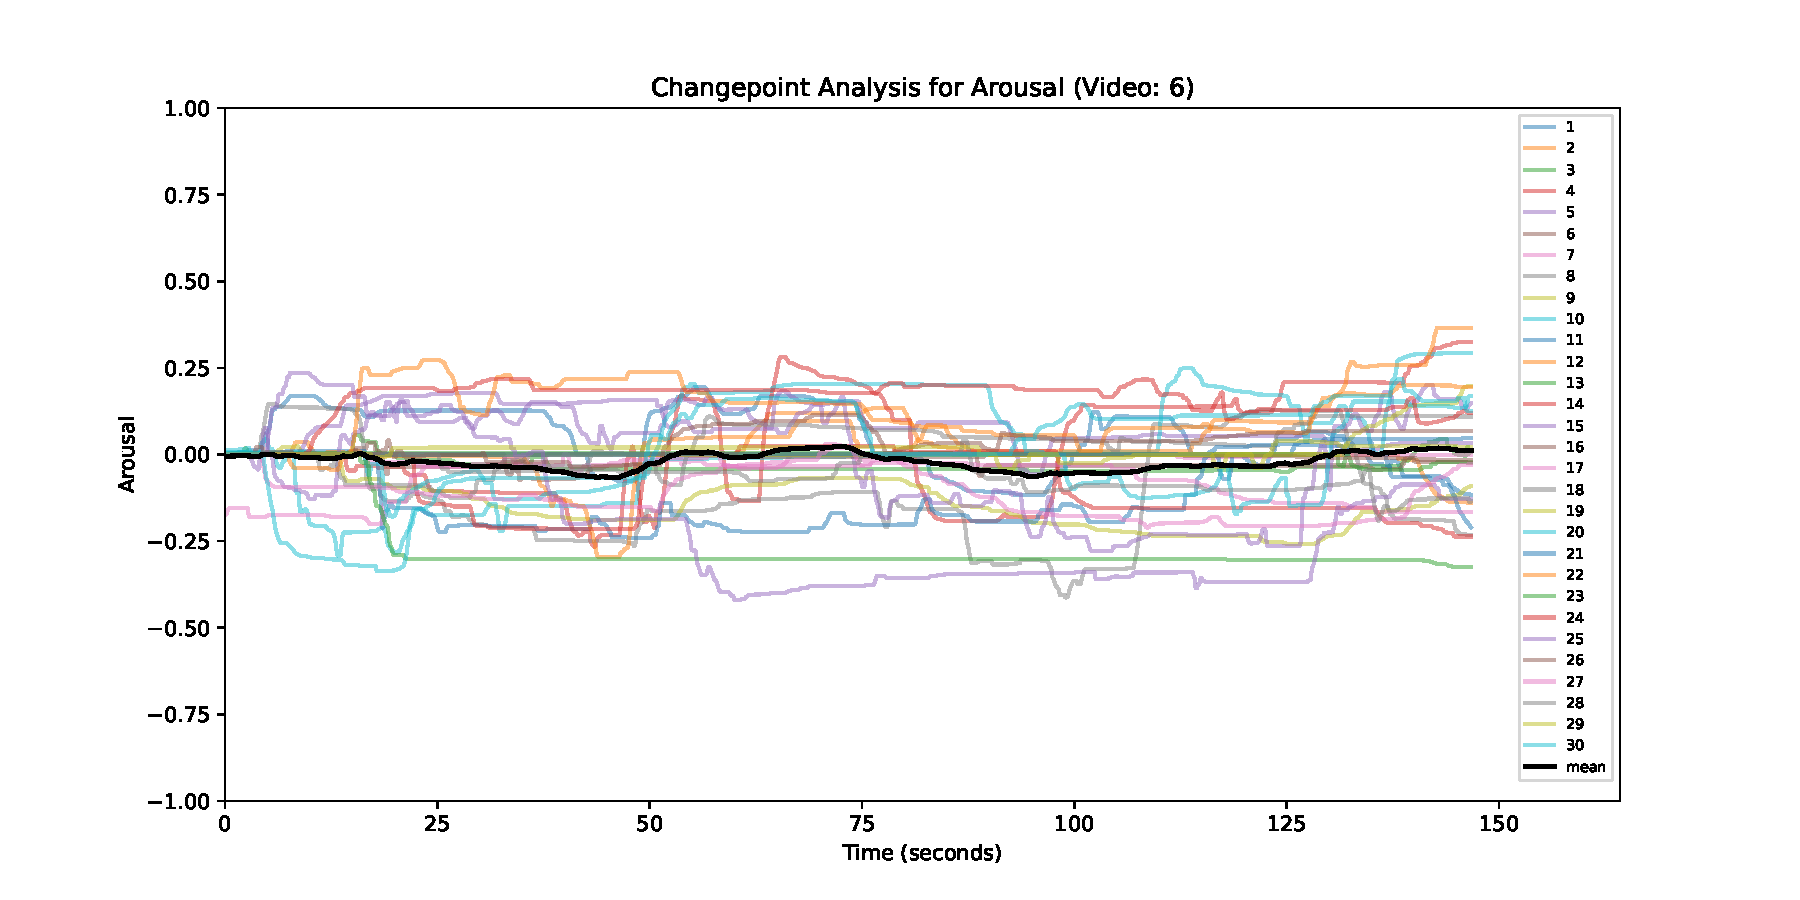
\includegraphics[width=\linewidth]{changepoints_V6_arousal_avg_all_data} 
        \caption{} \label{fig:changepoints_V6_arousal_avg_all_data}
    \end{subfigure}
    \hfill
    \begin{subfigure}[t]{0.49\textwidth}
        \centering
        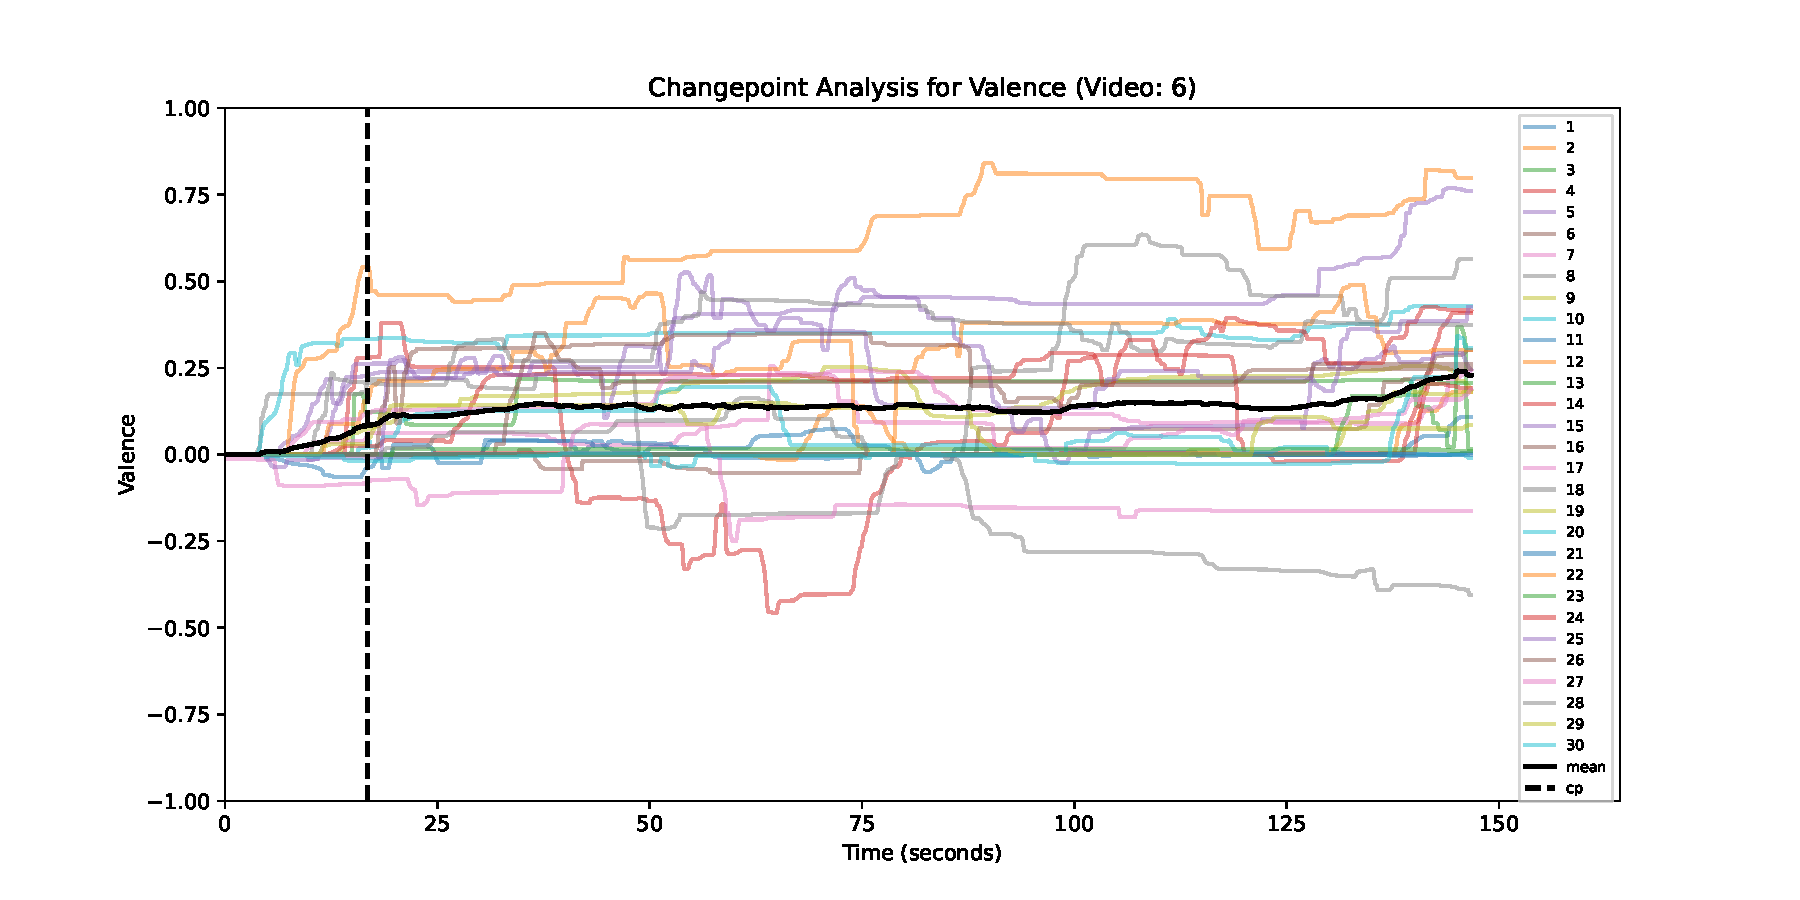
\includegraphics[width=\linewidth]{changepoints_V6_valence_avg_all_data} 
        \caption{} \label{fig:changepoints_V6_valence_avg_all_data}
    \end{subfigure}

    \vspace{1cm}
    
        \centering
    \begin{subfigure}[t]{0.49\textwidth}
        \centering
        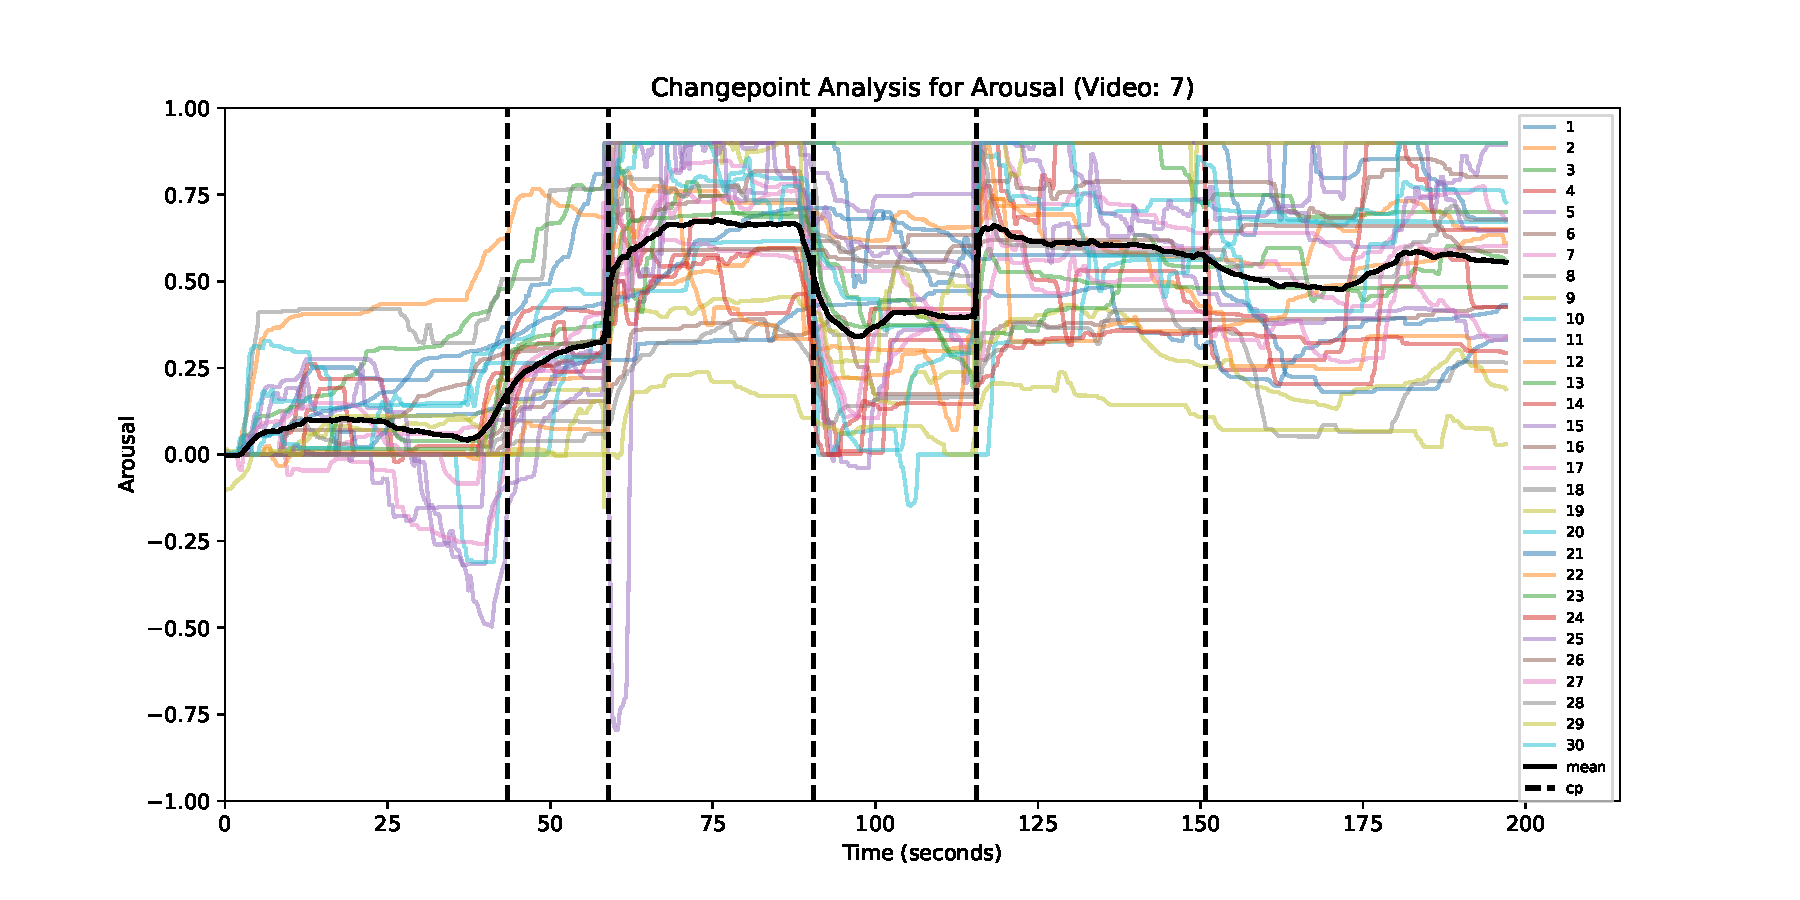
\includegraphics[width=\linewidth]{changepoints_V7_arousal_avg_all_data} 
        \caption{} \label{fig:changepoints_V7_arousal_avg_all_data}
    \end{subfigure}
    \hfill
    \begin{subfigure}[t]{0.49\textwidth}
        \centering
        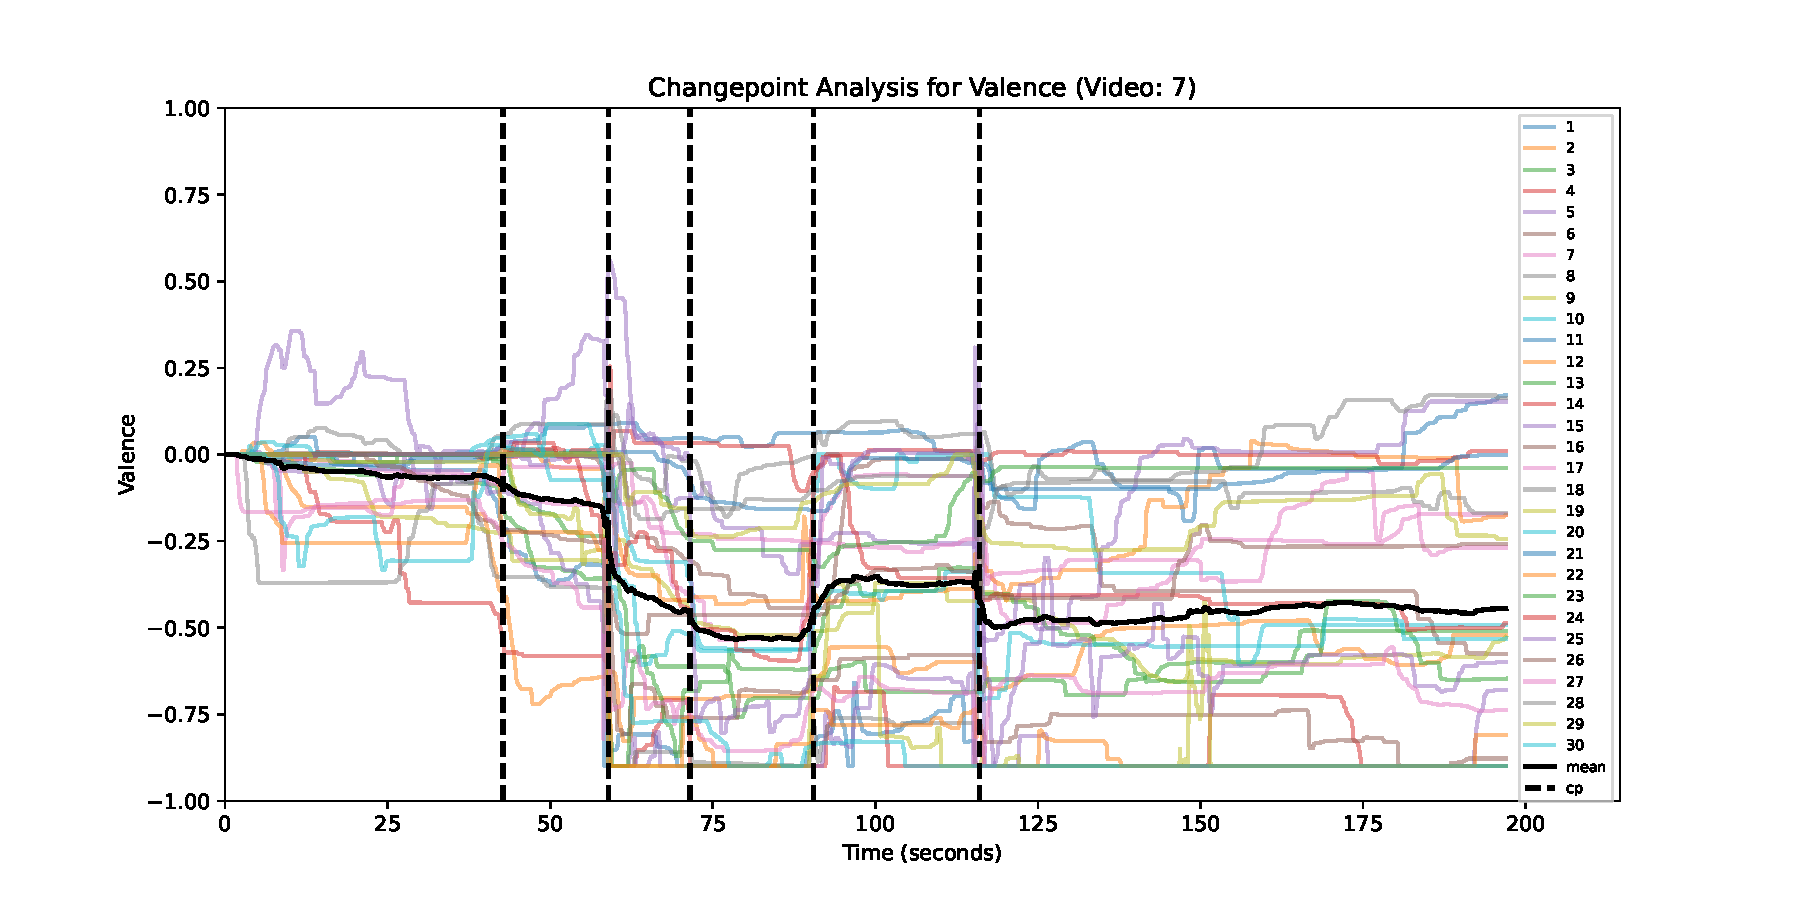
\includegraphics[width=\linewidth]{changepoints_V7_valence_avg_all_data} 
        \caption{} \label{fig:changepoints_V7_valence_avg_all_data}
    \end{subfigure}

    \vspace{1cm}
    
        \centering
    \begin{subfigure}[t]{0.49\textwidth}
        \centering
        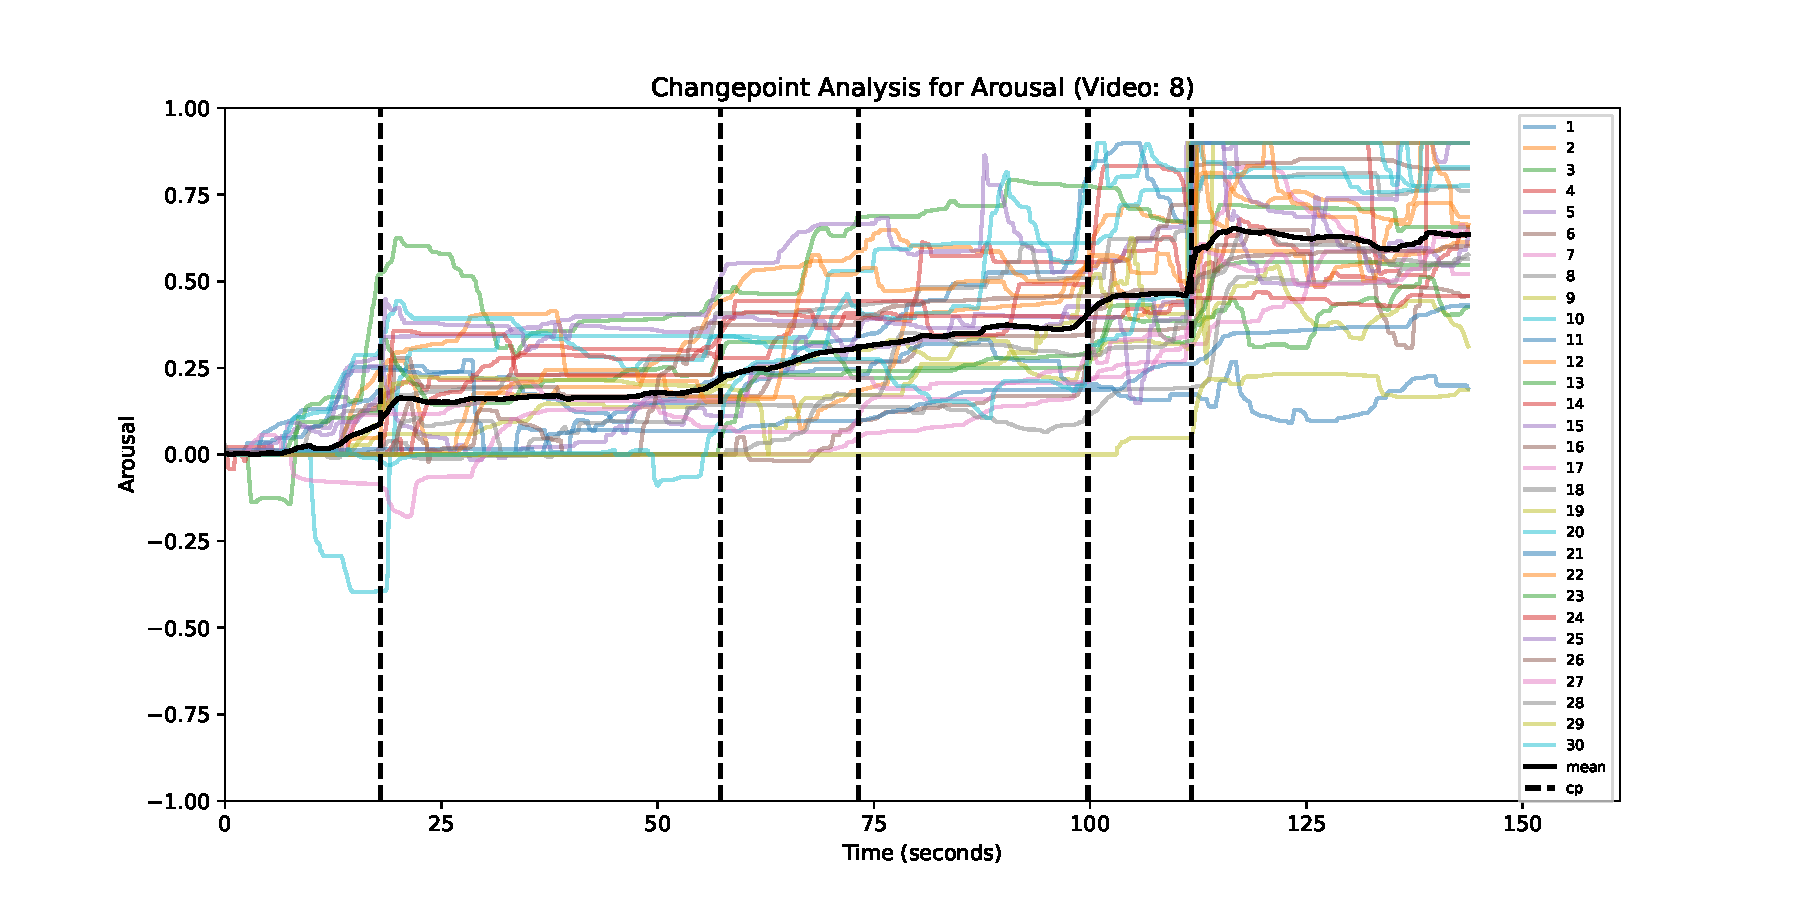
\includegraphics[width=\linewidth]{changepoints_V8_arousal_avg_all_data} 
        \caption{} \label{fig:changepoints_V8_arousal_avg_all_data}
    \end{subfigure}
    \hfill
    \begin{subfigure}[t]{0.49\textwidth}
        \centering
        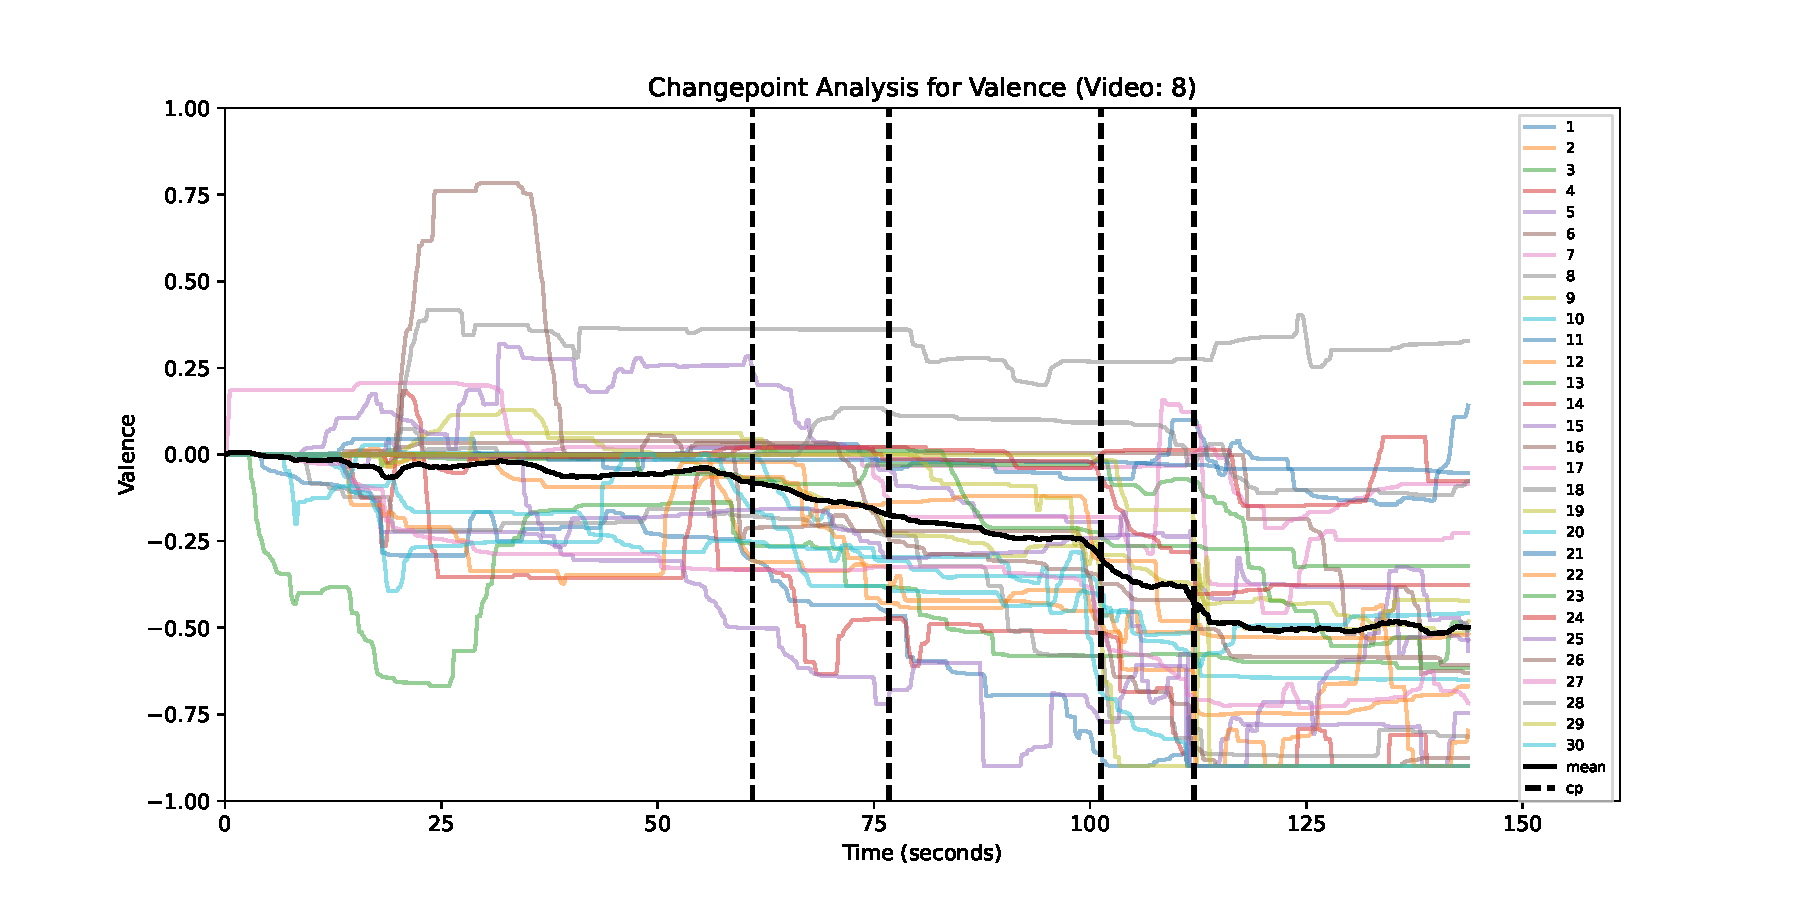
\includegraphics[width=\linewidth]{changepoints_V8_valence_avg_all_data} 
        \caption{} \label{fig:changepoints_V8_valence_avg_all_data}
    \end{subfigure}
    
    \caption{\textit{Change points in arousal and valence ratings for all videos averaged across subjects} Change points as identified by the algorithm for each video's arousal (left column) and valence (right column) ratings averaged across subjects. Black dashed lines indicate the change points. Colored lines indicate the ratings of the different participants, the thick black line is the mean rating. Even though the algorithm seems to be able to identify change points in all videos, only video 7 and video 8 (high arousal and negative valence) seemed to have significant changes in valence and arousal ratings. Note the different lengths of the videos.}
    \label{fig:all_data}
\end{figure}

% table cpa timestamps
\begin{table}[]
\centering
\caption{\textit{X-Coordinates (timestamps) of change points for all videos averaged across participants.} Q = Quadrant (video category); HP = high arousal and positive valence; LN = low arousal and negative valence; LP = low arousal and positive valence; HN = high arousal and negative valence; CP = change point; No. = number.}
\label{tab:table_avg_cpa}
\resizebox{\textwidth}{!}{%
\begin{tabular}{llccccccc}
\hline
\textbf{Video} & \textbf{Q} & \textbf{CP Valence} & \textbf{No. CP Valence} & \textbf{CP Arousal} & \textbf{No. CP Arousal} & \textbf{Model} & \textbf{Jump} & \textbf{Penalty} \\ \hline
1 & HP & {[}5.5, 32.75, 145.0{]} & 3 & {[}138.5{]} & 1 & l2 & 5 & 1 \\
2 & HP & {[}13.75, 61.25, 116.5, 141.25{]} & 4 & {[}117.75{]} & 1 & l2 & 5 & 1 \\
3 & LN & {[}45.0{]} & 1 & {[}19.75, 42.5{]} & 2 & l2 & 5 & 1 \\
4 & LN & {[}{]} & 0 & {[}20.5, 68.25{]} & 2 & l2 & 5 & 1 \\
5 & LP & {[}7.0, 101.5{]} & 2 & {[}37.75, 59.75, 95.5{]} & 3 & l2 & 5 & 1 \\
6 & LP & {[}16.75{]} & 1 & {[}{]} & 0 & l2 & 5 & 1 \\
7 & HN & {[}42.75, 59.0, 71.5, 90.5, 116.0{]} & 5 & {[}43.5, 59.0, 90.5, 115.5, 150.75{]} & 5 & l2 & 5 & 1 \\
8 & HN & {[}61.0, 76.75, 101.25, 112.0{]} & 4 & {[}18.0, 57.25, 73.25, 99.75, 111.75{]} & 5 & l2 & 5 & 1 \\ \hline
\end{tabular}%
}
\end{table}

\newpage

% +++++ subsection cpa with mean timeseries but for all participants ++++++
\subsection{CPA for data averaged across participants but with individual change points}
Figure \ref{fig:all} shows the shows the change points identified for each video's arousal and valence ratings for all subjects in one plot to show the interindividual differences in change points. Additionally, the mean timeseries for valence and arousal and the mean change points for all participants are depicted. We can see that there are high differences both in the number and in the point in time of change points between participants. Only in video 7 and 8, there seems to be a bigger congruence of participants' data. As already mentioned, these videos were the ones labelled as 'scary' by the authors. One explanation for this pattern is that these scary videos succeded in eliciting more similiar emotional reactions across participants than the positive and low arousing videos where participants differed more in both timing and magnitude of changes in annotation data.

% figure cpa all change points
\begin{figure}
    \centering
    \begin{subfigure}[t]{0.49\textwidth}
        \centering
        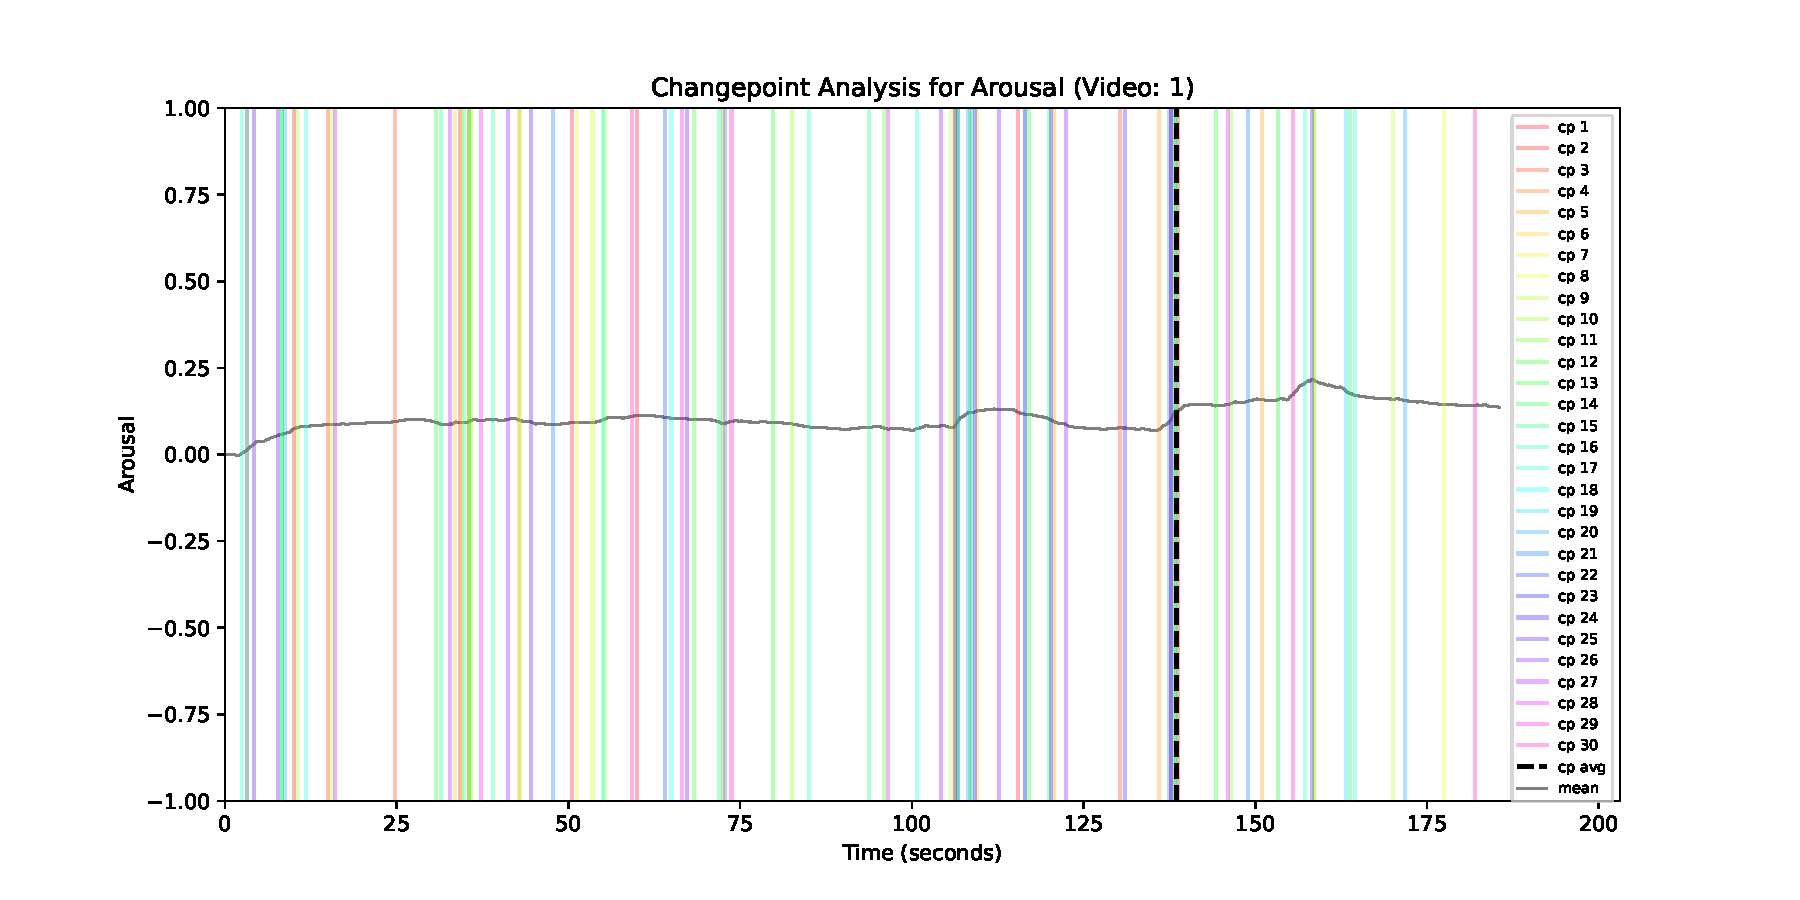
\includegraphics[width=\linewidth]{changepoints_V1_arousal_avg} 
        \caption{} \label{fig:changepoints_V1_arousal_avg}
    \end{subfigure}
    \hfill
    \begin{subfigure}[t]{0.49\textwidth}
        \centering
        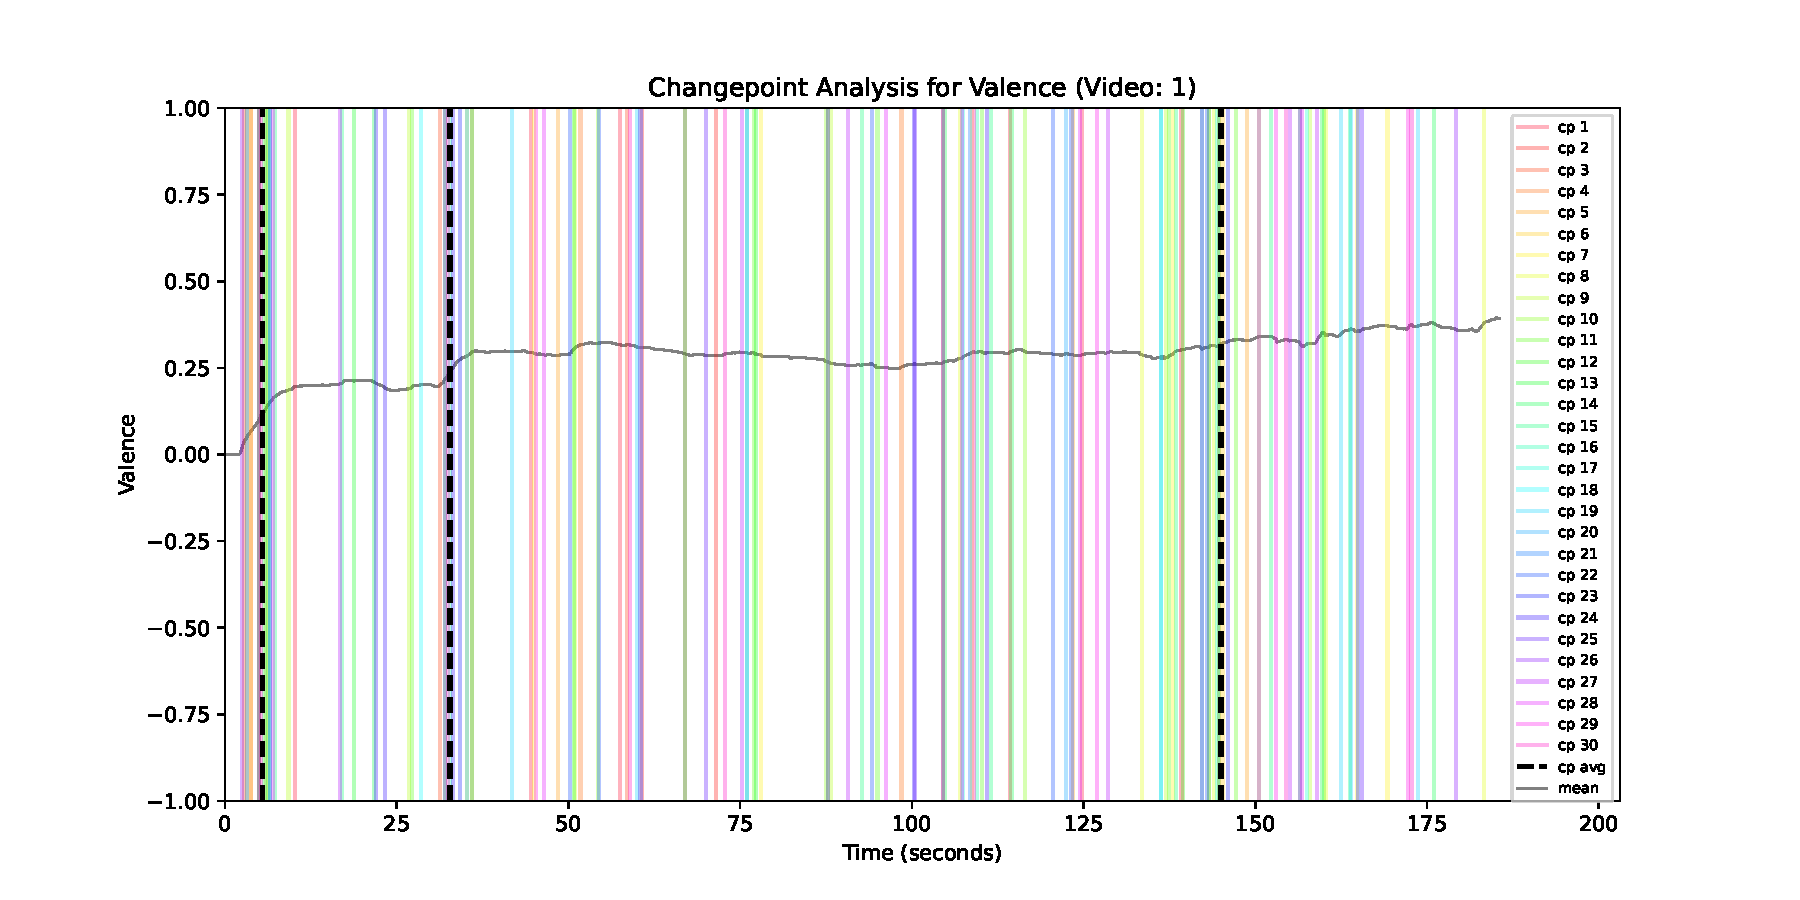
\includegraphics[width=\linewidth]{changepoints_V1_valence_avg} 
        \caption{} \label{fig:changepoints_V1_valence_avg}
    \end{subfigure}

    \vspace{1cm}
    
    \centering
    \begin{subfigure}[t]{0.49\textwidth}
        \centering
        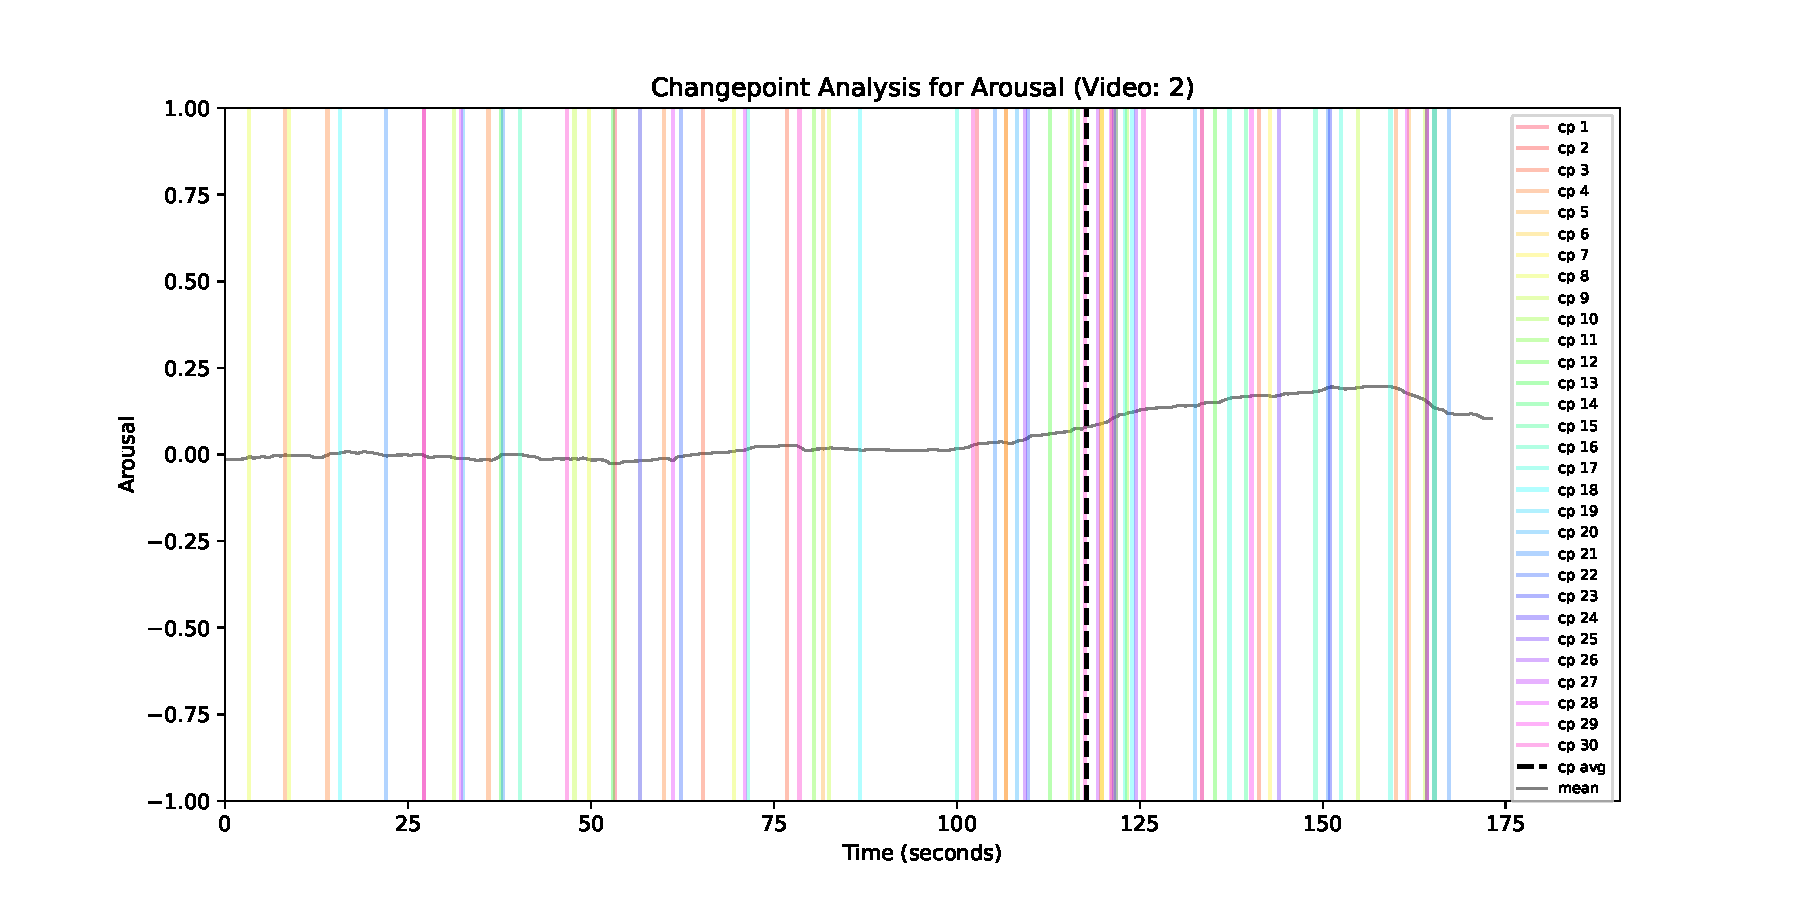
\includegraphics[width=\linewidth]{changepoints_V2_arousal_avg} 
        \caption{} \label{fig:changepoints_V2_arousal_avg}
    \end{subfigure}
    \hfill
    \begin{subfigure}[t]{0.49\textwidth}
        \centering
        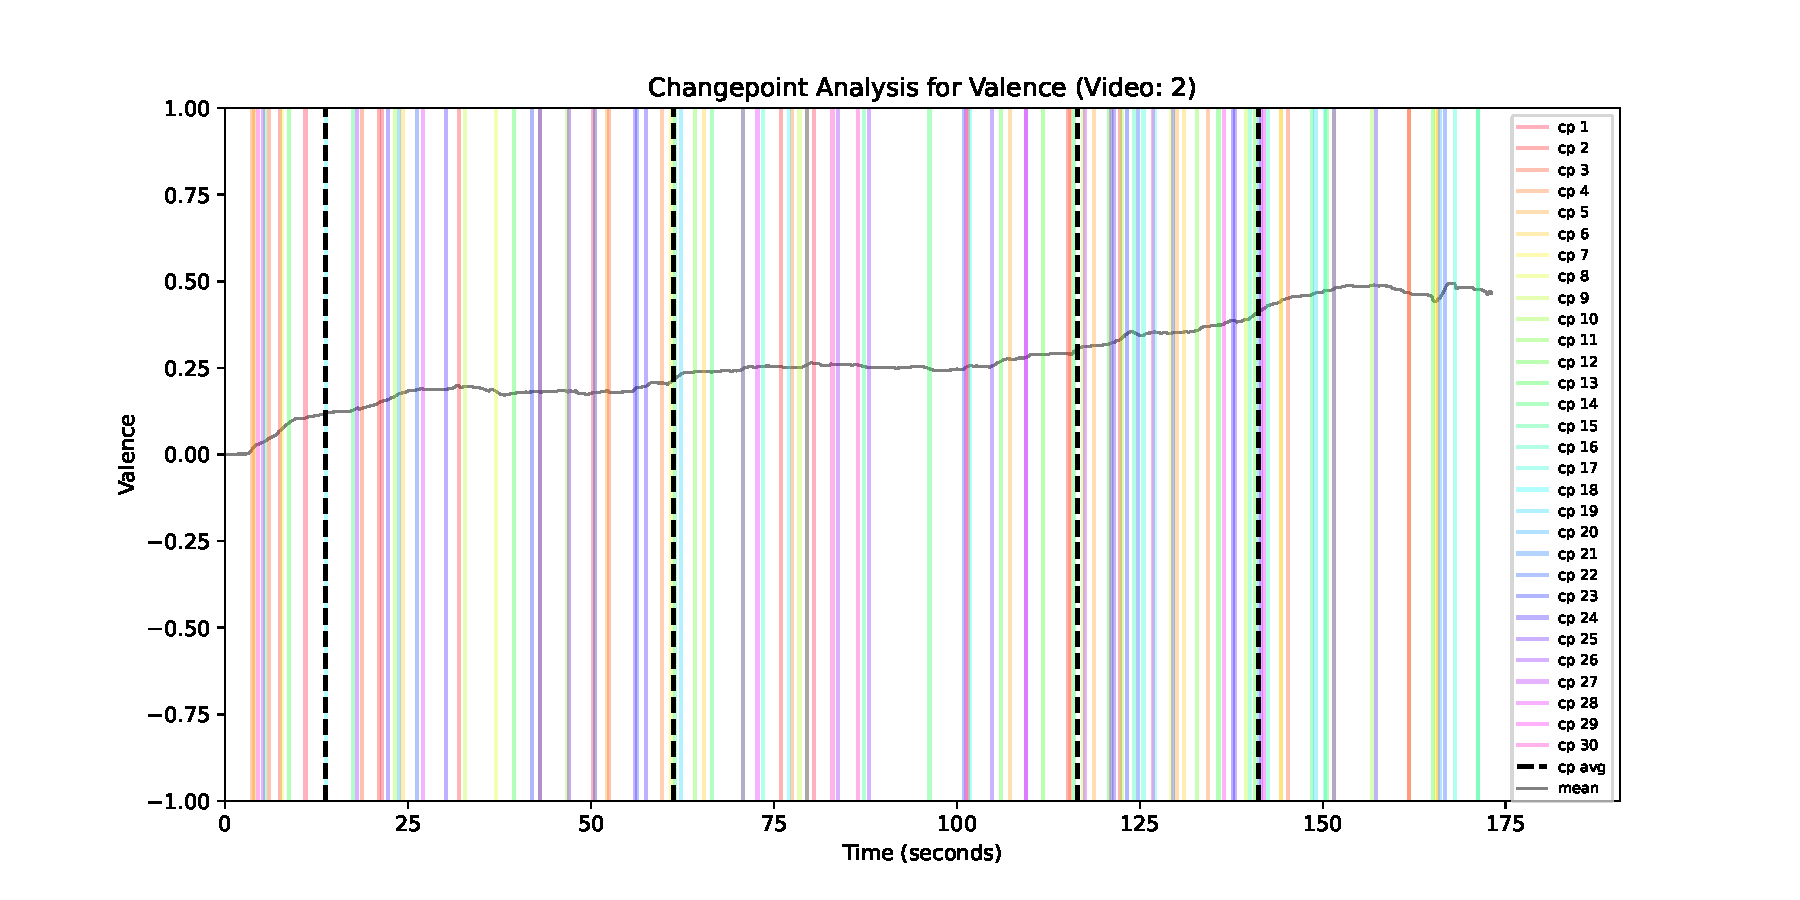
\includegraphics[width=\linewidth]{changepoints_V2_valence_avg} 
        \caption{} \label{fig:changepoints_V2_valence_avg}
    \end{subfigure}
    
        \centering
    \begin{subfigure}[t]{0.49\textwidth}
        \centering
        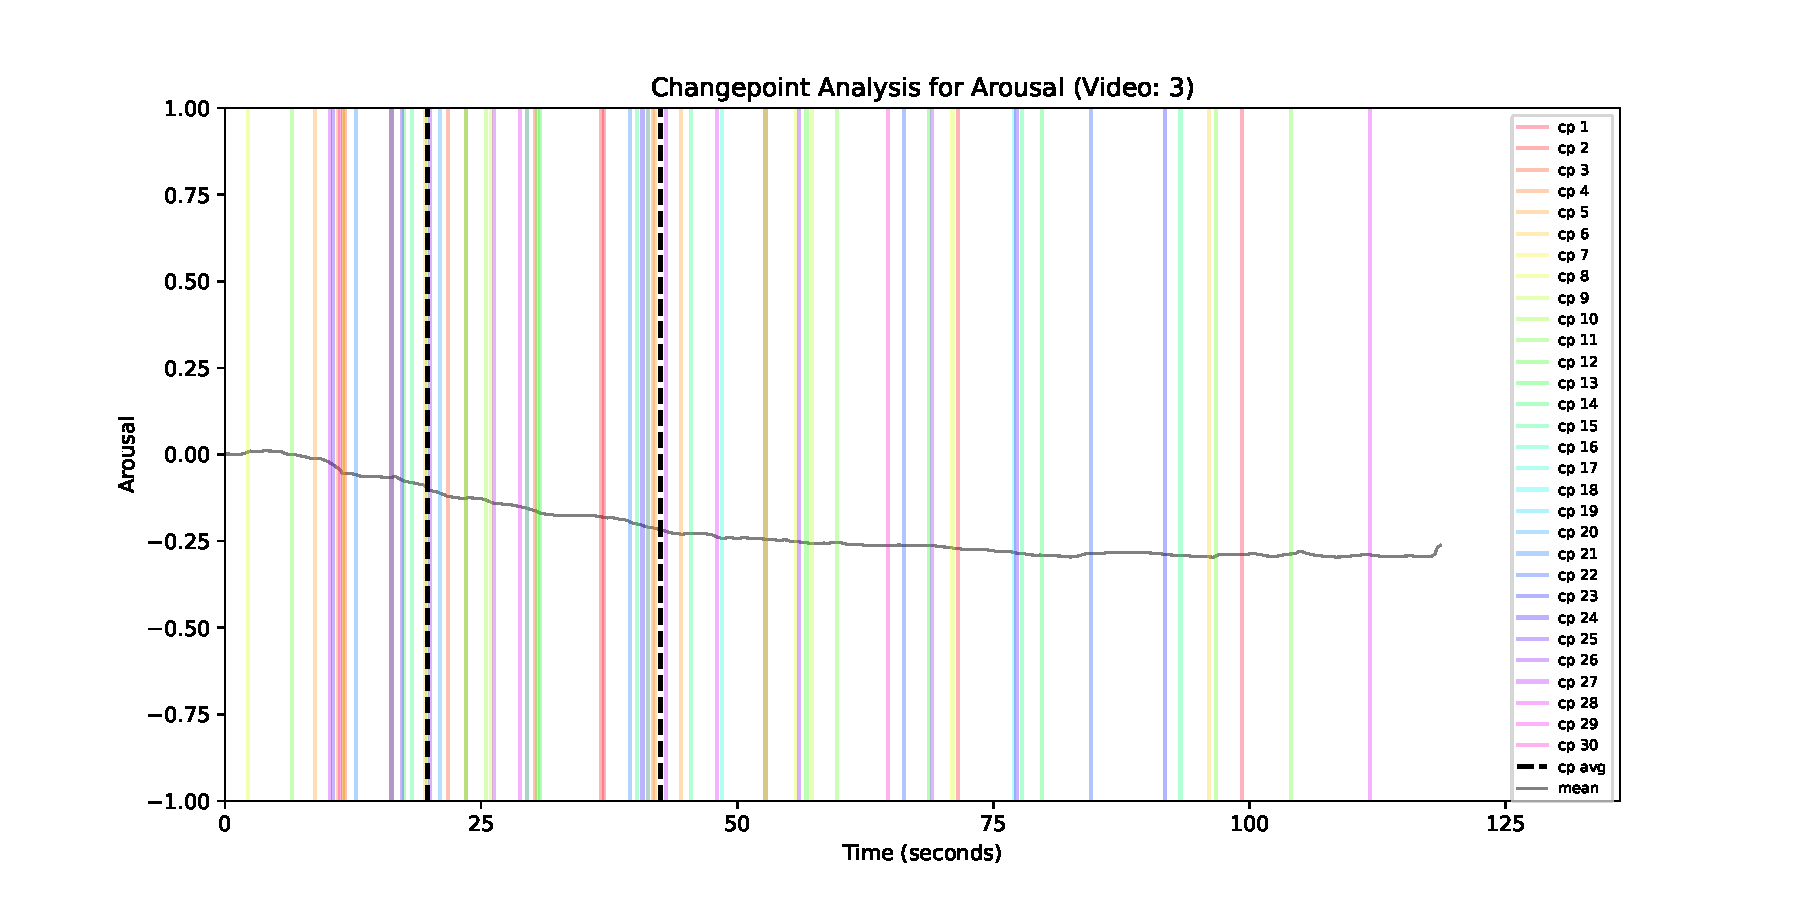
\includegraphics[width=\linewidth]{changepoints_V3_arousal_avg} 
        \caption{} \label{fig:changepoints_V3_arousal_avg}
    \end{subfigure}
    \hfill
    \begin{subfigure}[t]{0.49\textwidth}
        \centering
        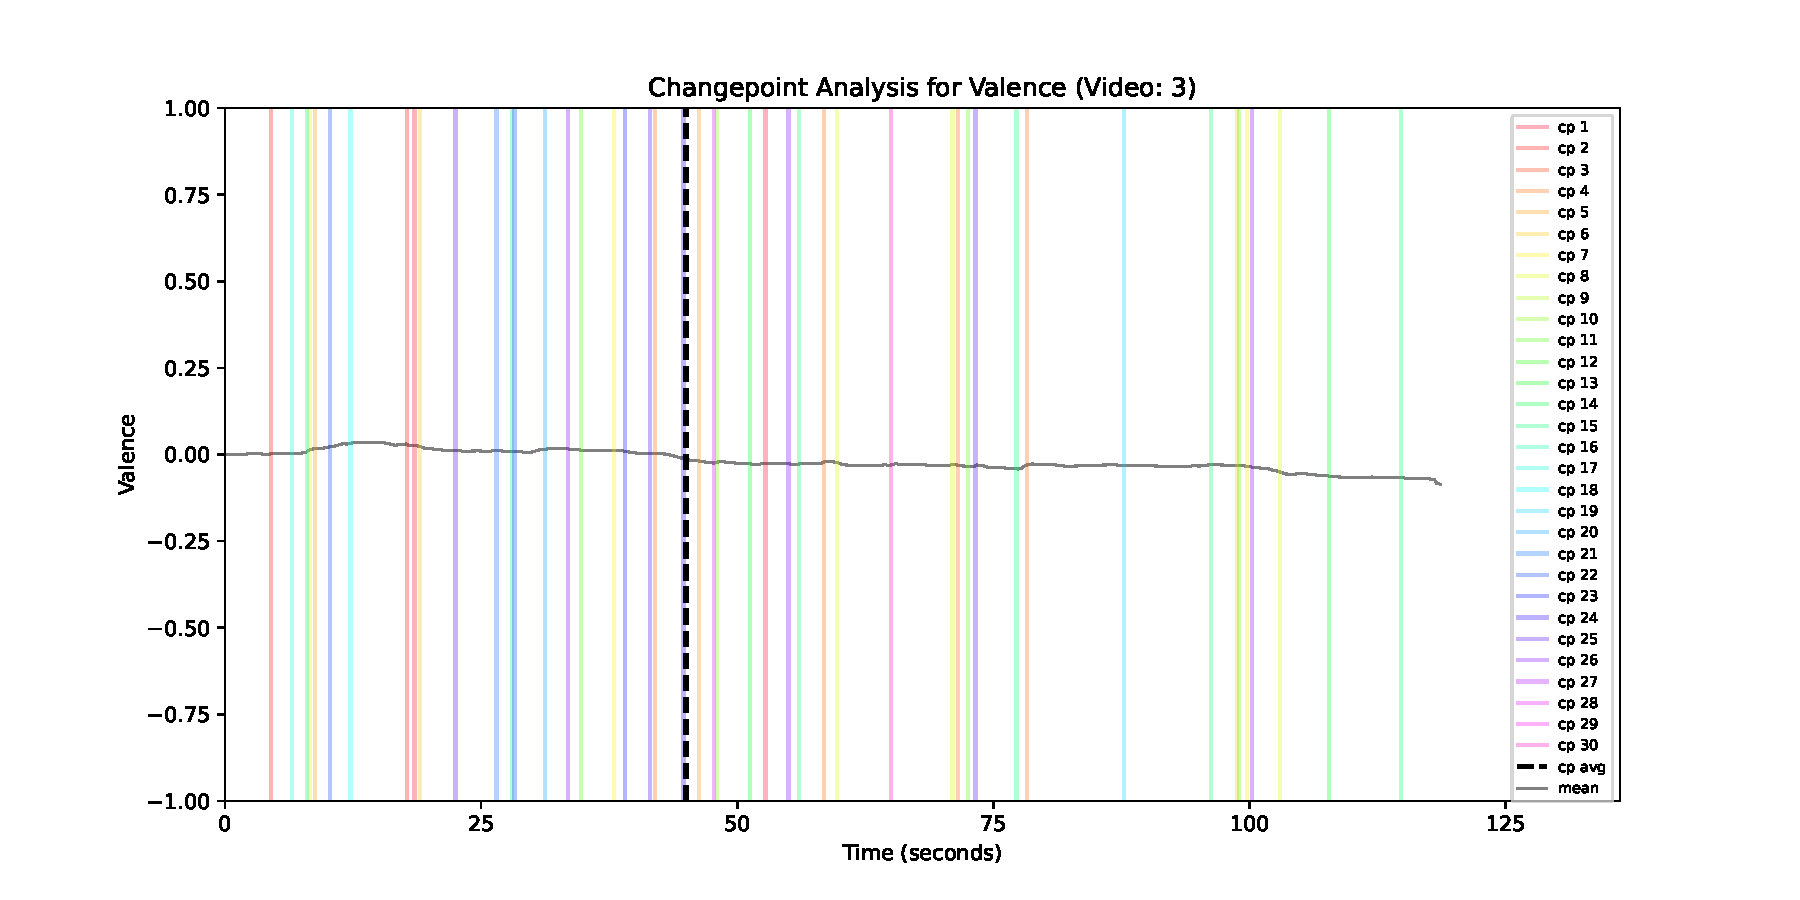
\includegraphics[width=\linewidth]{changepoints_V3_valence_avg} 
        \caption{} \label{fig:changepoints_V3_valence_avg}
    \end{subfigure}

    \vspace{1cm}
    
        \centering
    \begin{subfigure}[t]{0.49\textwidth}
        \centering
        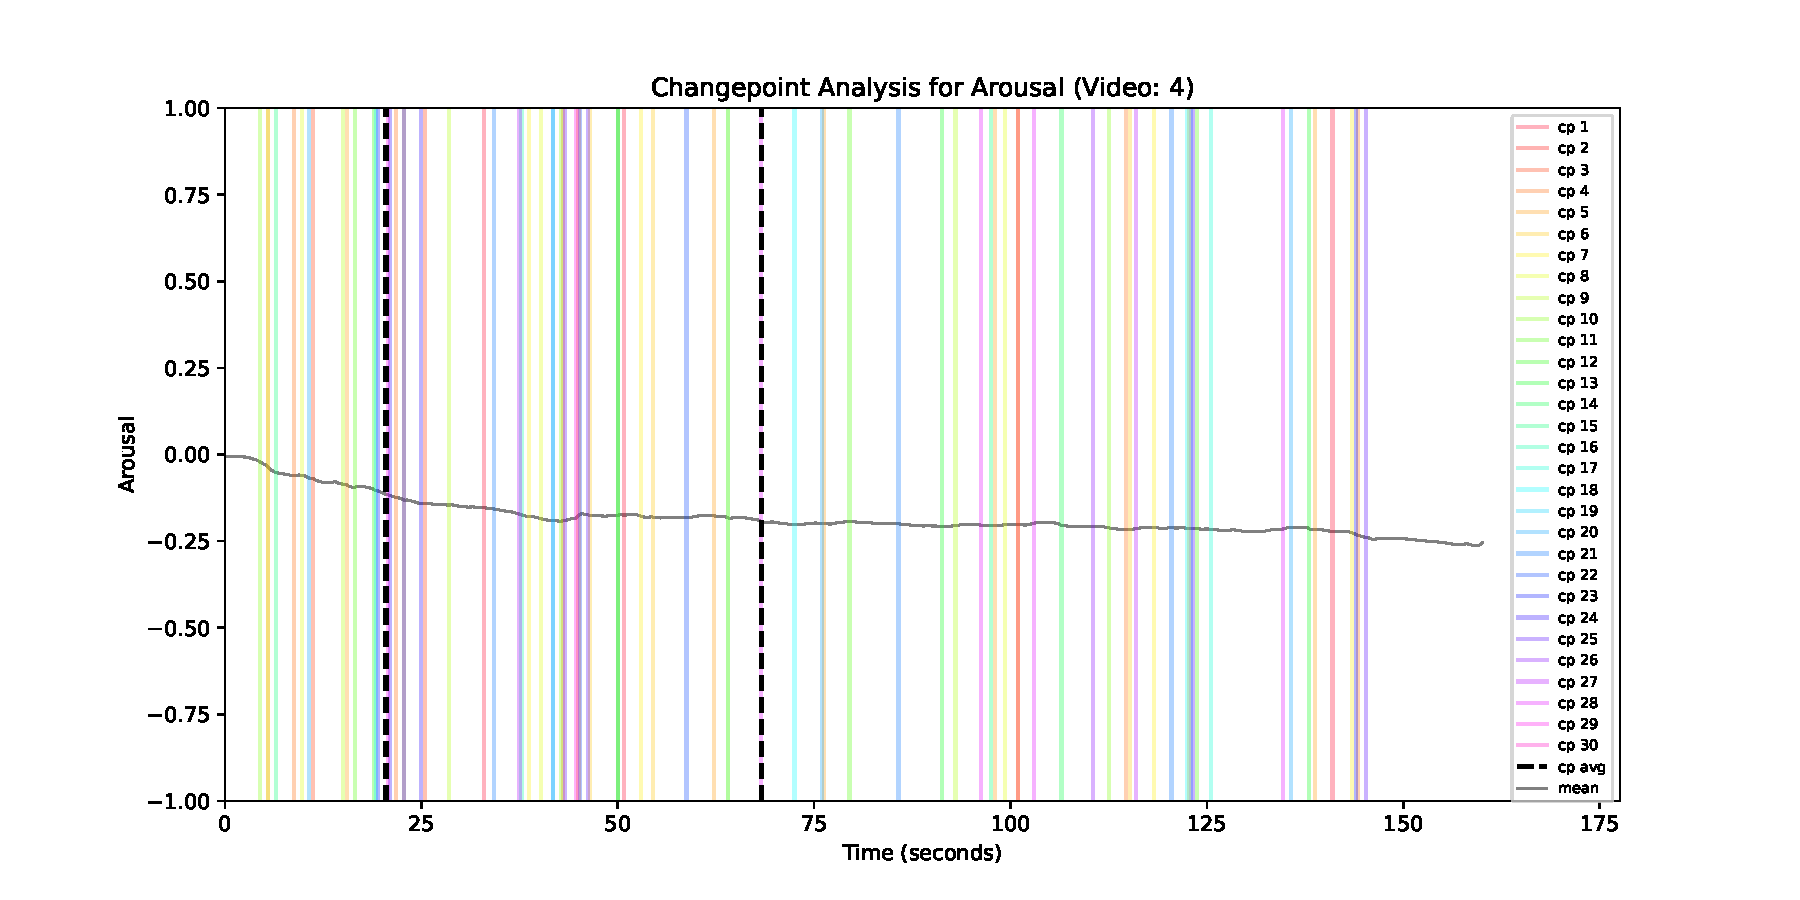
\includegraphics[width=\linewidth]{changepoints_V4_arousal_avg} 
        \caption{} \label{fig:changepoints_V4_arousal_avg}
    \end{subfigure}
    \hfill
    \begin{subfigure}[t]{0.49\textwidth}
        \centering
        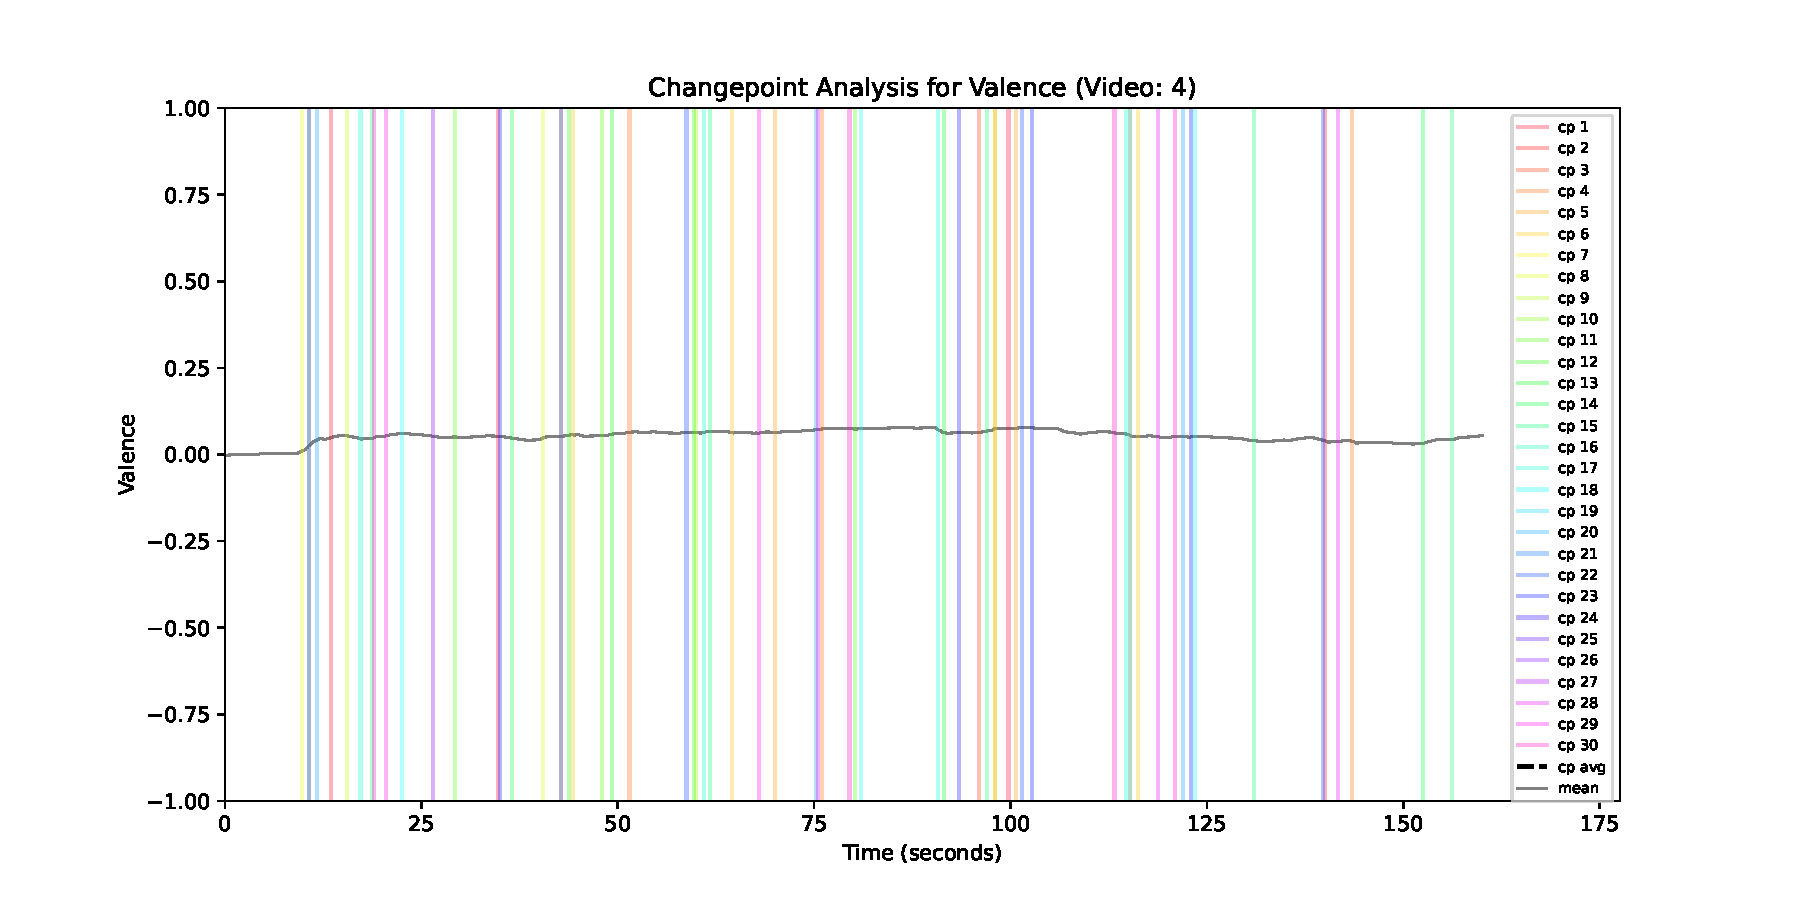
\includegraphics[width=\linewidth]{changepoints_V4_valence_avg} 
        \caption{} \label{fig:changepoints_V4_valence_avg}
    \end{subfigure}
 \end{figure}

  \begin{figure} \ContinuedFloat
        \centering
    \begin{subfigure}[t]{0.49\textwidth}
        \centering
        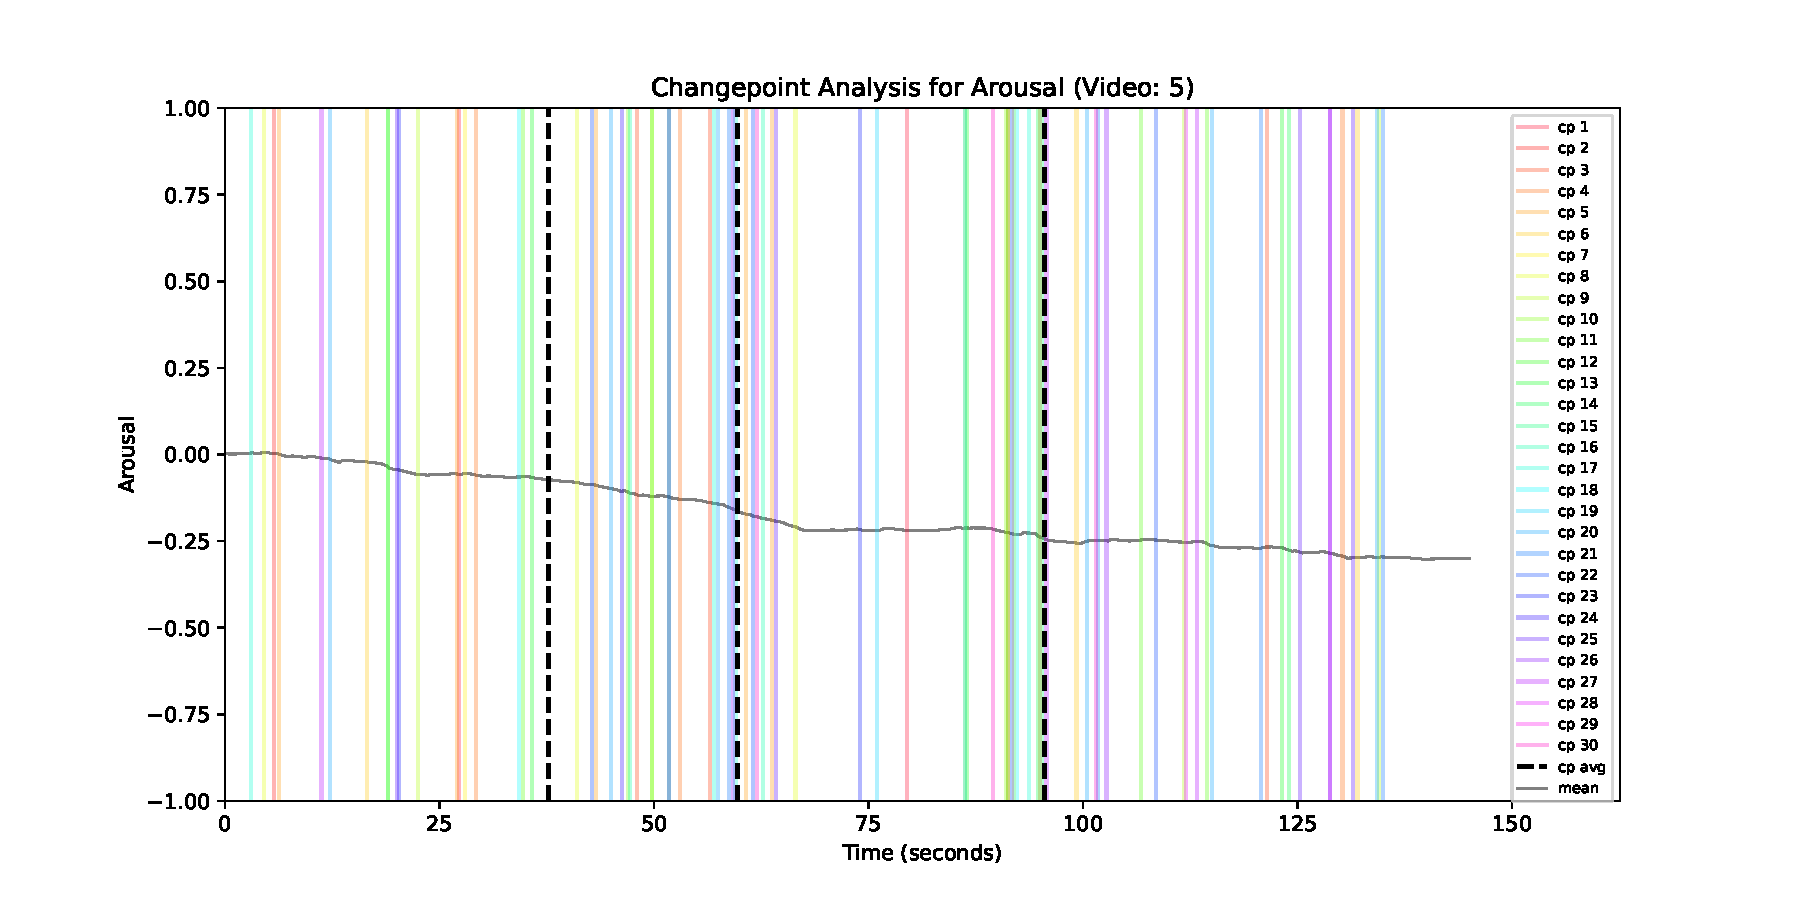
\includegraphics[width=\linewidth]{changepoints_V5_arousal_avg}
        \caption{} \label{fig:changepoints_V5_arousal_avg}
    \end{subfigure}
    \hfill
    \begin{subfigure}[t]{0.49\textwidth}
        \centering
        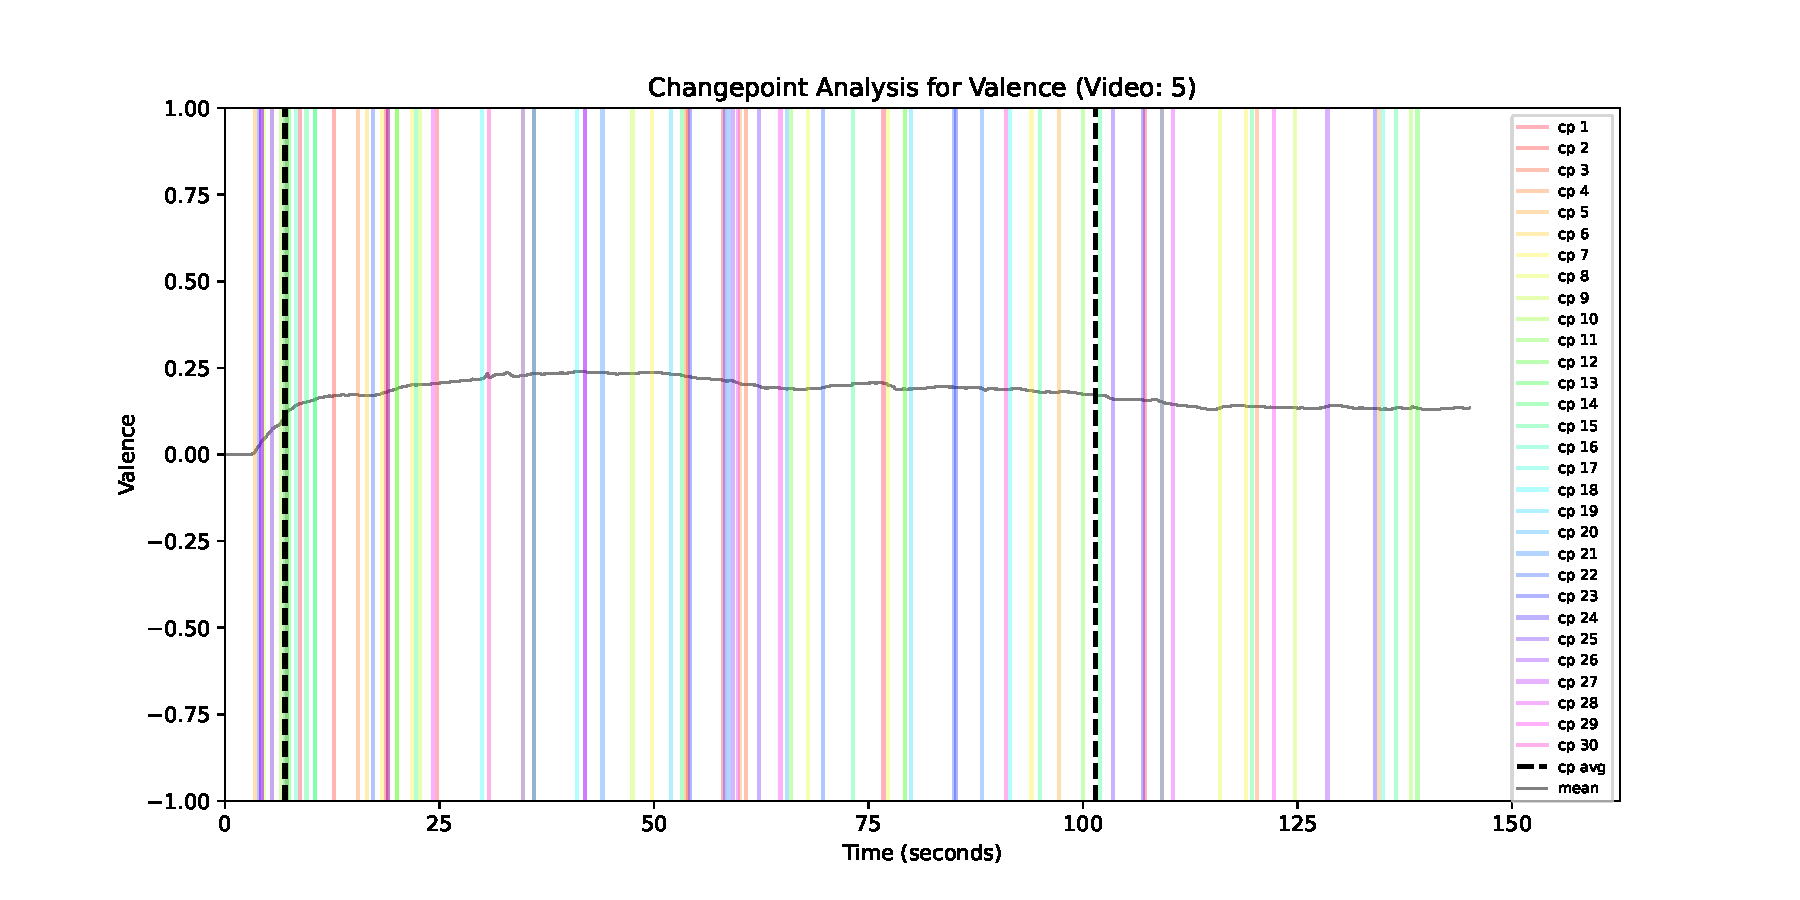
\includegraphics[width=\linewidth]{changepoints_V5_valence_avg} 
        \caption{} \label{fig:changepoints_V5_valence_avg}
    \end{subfigure}

    \vspace{1cm}
    
        \centering
    \begin{subfigure}[t]{0.49\textwidth}
        \centering
        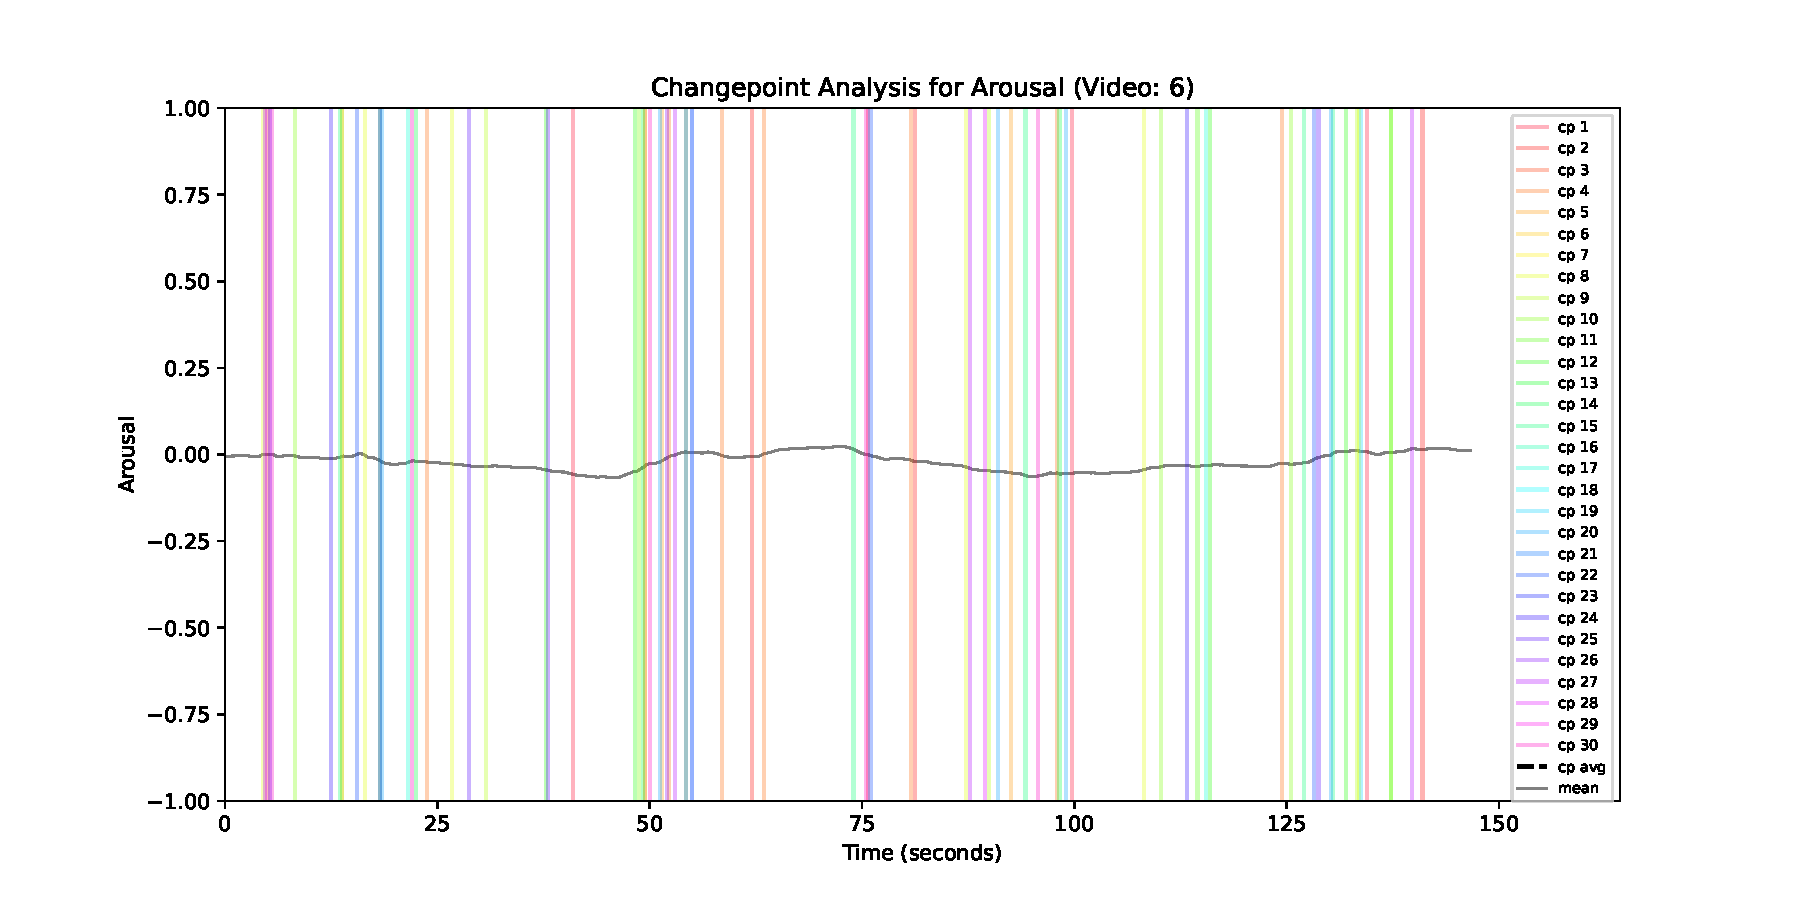
\includegraphics[width=\linewidth]{changepoints_V6_arousal_avg} 
        \caption{} \label{fig:changepoints_V6_arousal_avg}
    \end{subfigure}
    \hfill
    \begin{subfigure}[t]{0.49\textwidth}
        \centering
        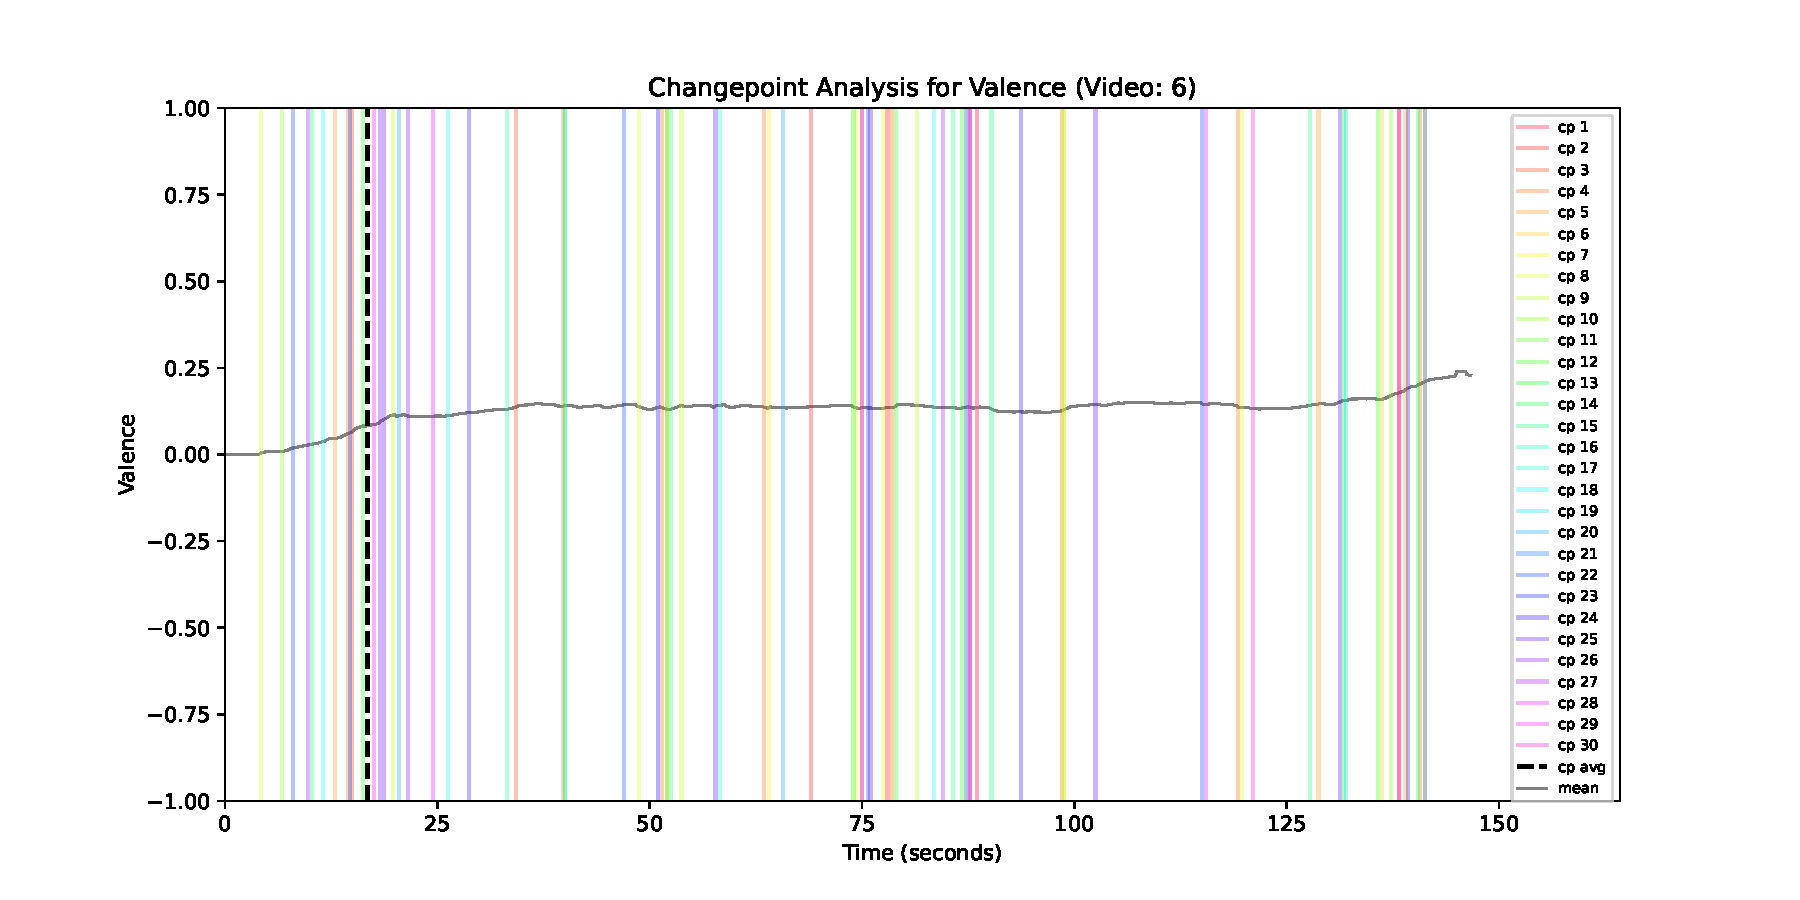
\includegraphics[width=\linewidth]{changepoints_V6_valence_avg} 
        \caption{} \label{fig:changepoints_V6_valence_avg}
    \end{subfigure}

    \vspace{1cm}
    
        \centering
    \begin{subfigure}[t]{0.49\textwidth}
        \centering
        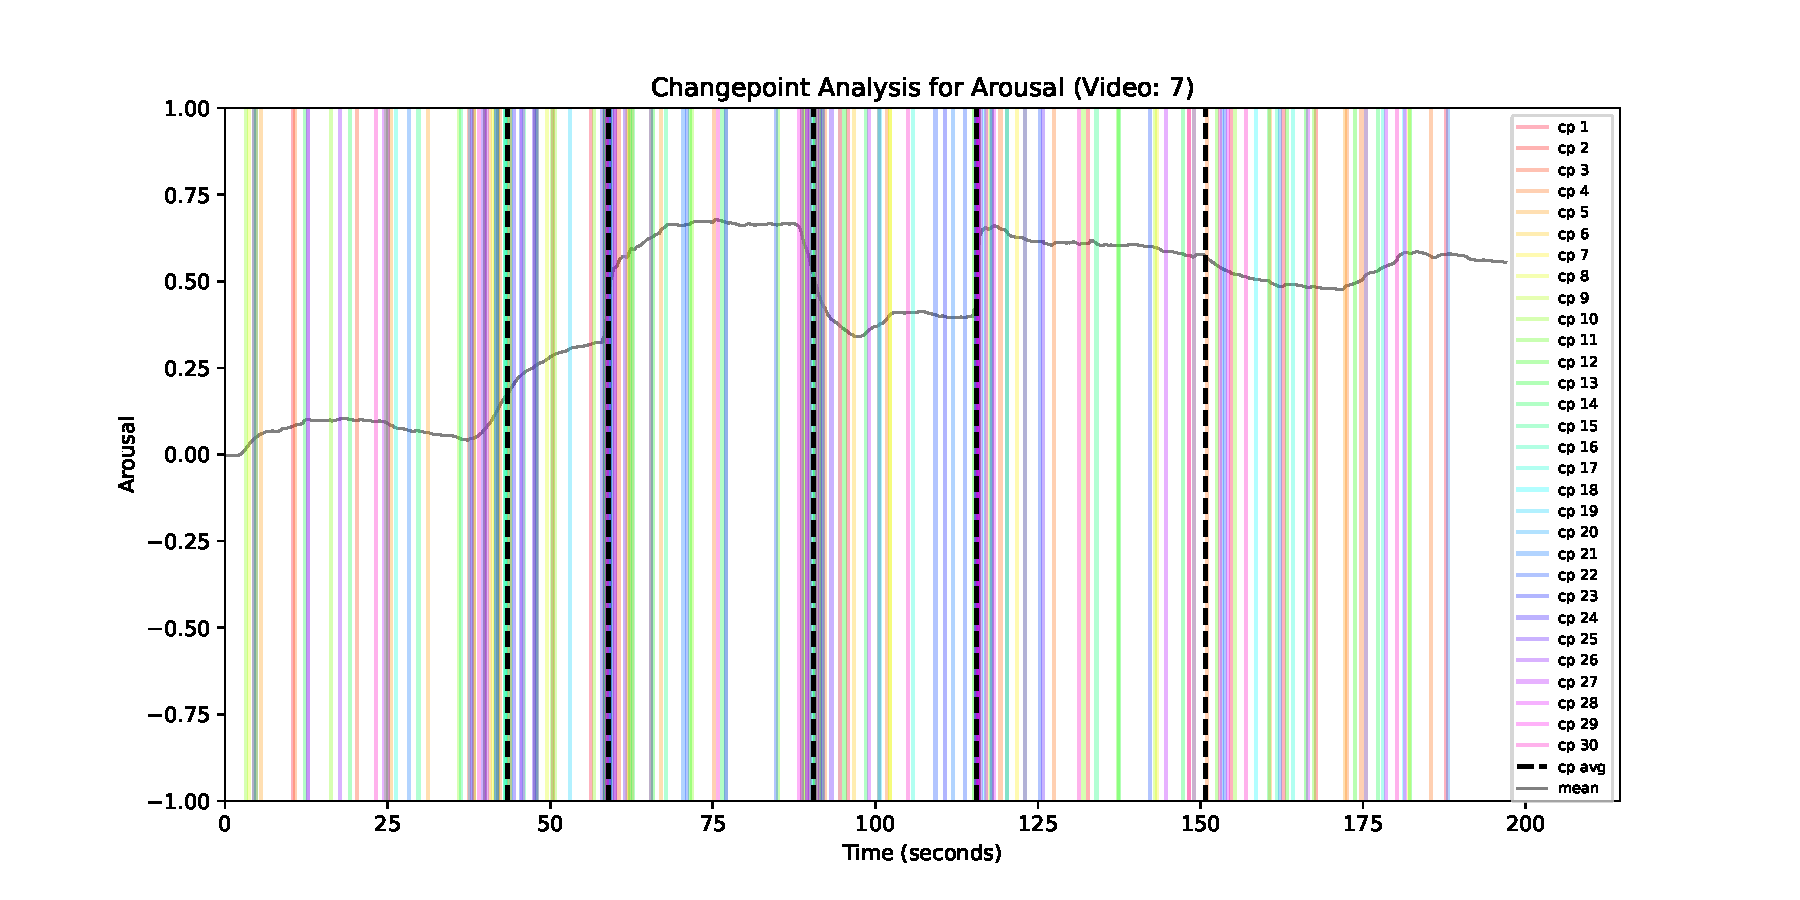
\includegraphics[width=\linewidth]{changepoints_V7_arousal_avg} 
        \caption{} \label{fig:changepoints_V7_arousal_avg}
    \end{subfigure}
    \hfill
    \begin{subfigure}[t]{0.49\textwidth}
        \centering
        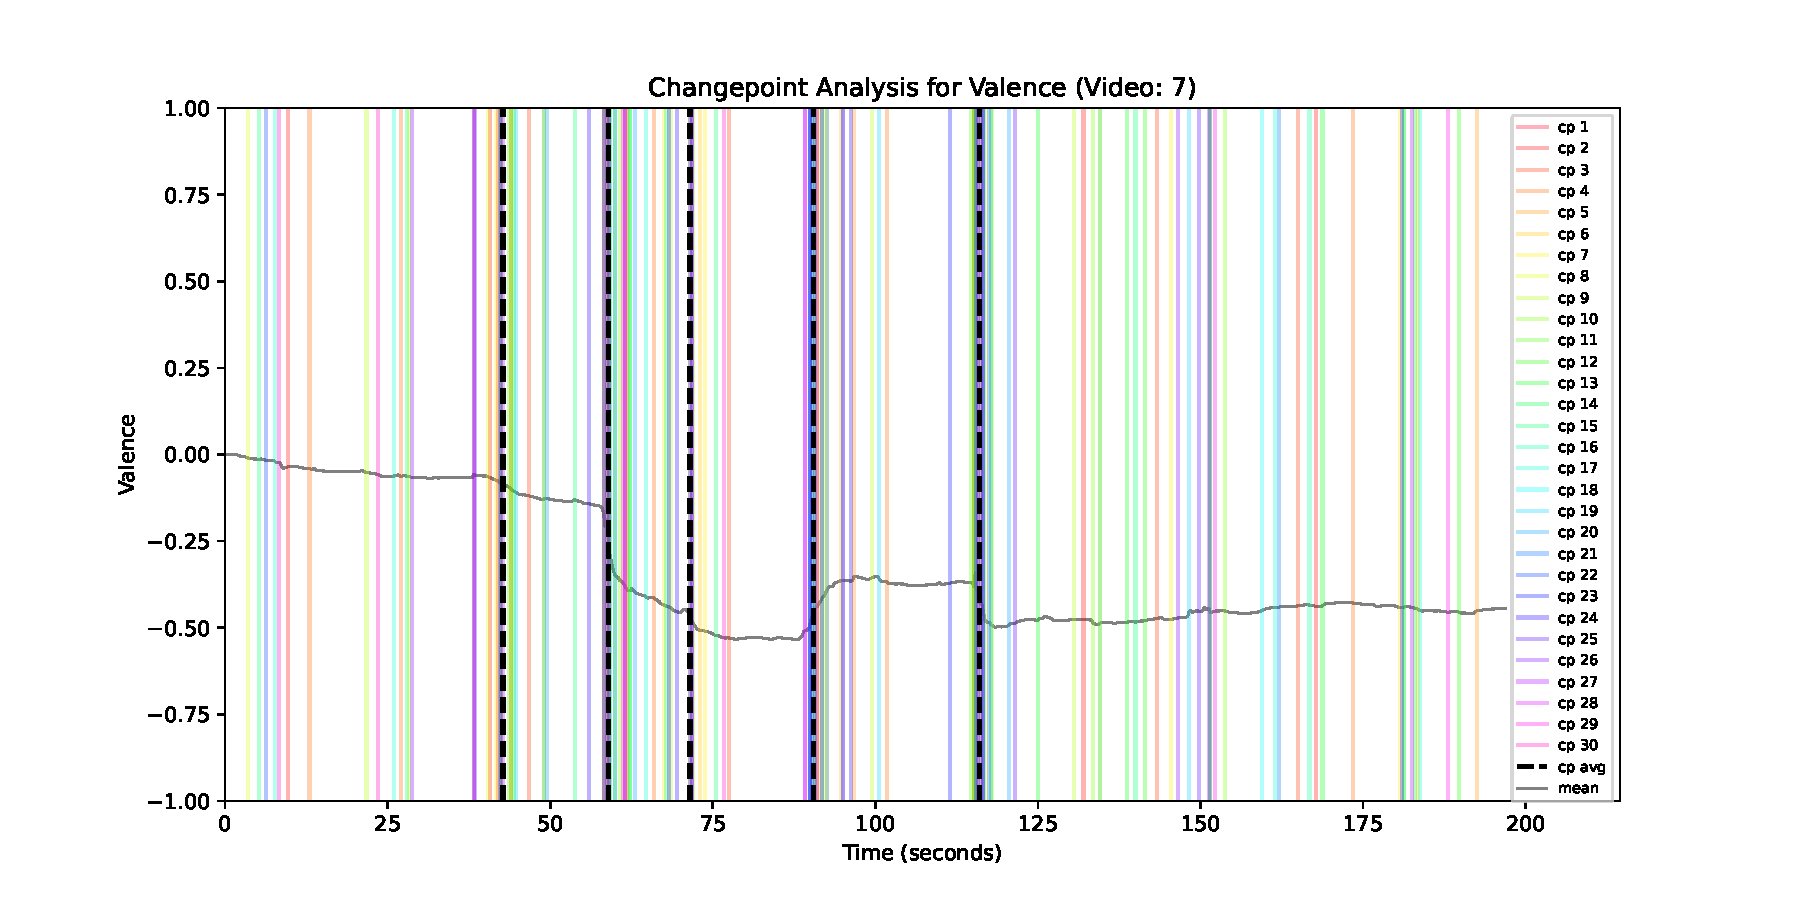
\includegraphics[width=\linewidth]{changepoints_V7_valence_avg} 
        \caption{} \label{fig:changepoints_V7_valence_avg}
    \end{subfigure}

    \vspace{1cm}
    
        \centering
    \begin{subfigure}[t]{0.49\textwidth}
        \centering
        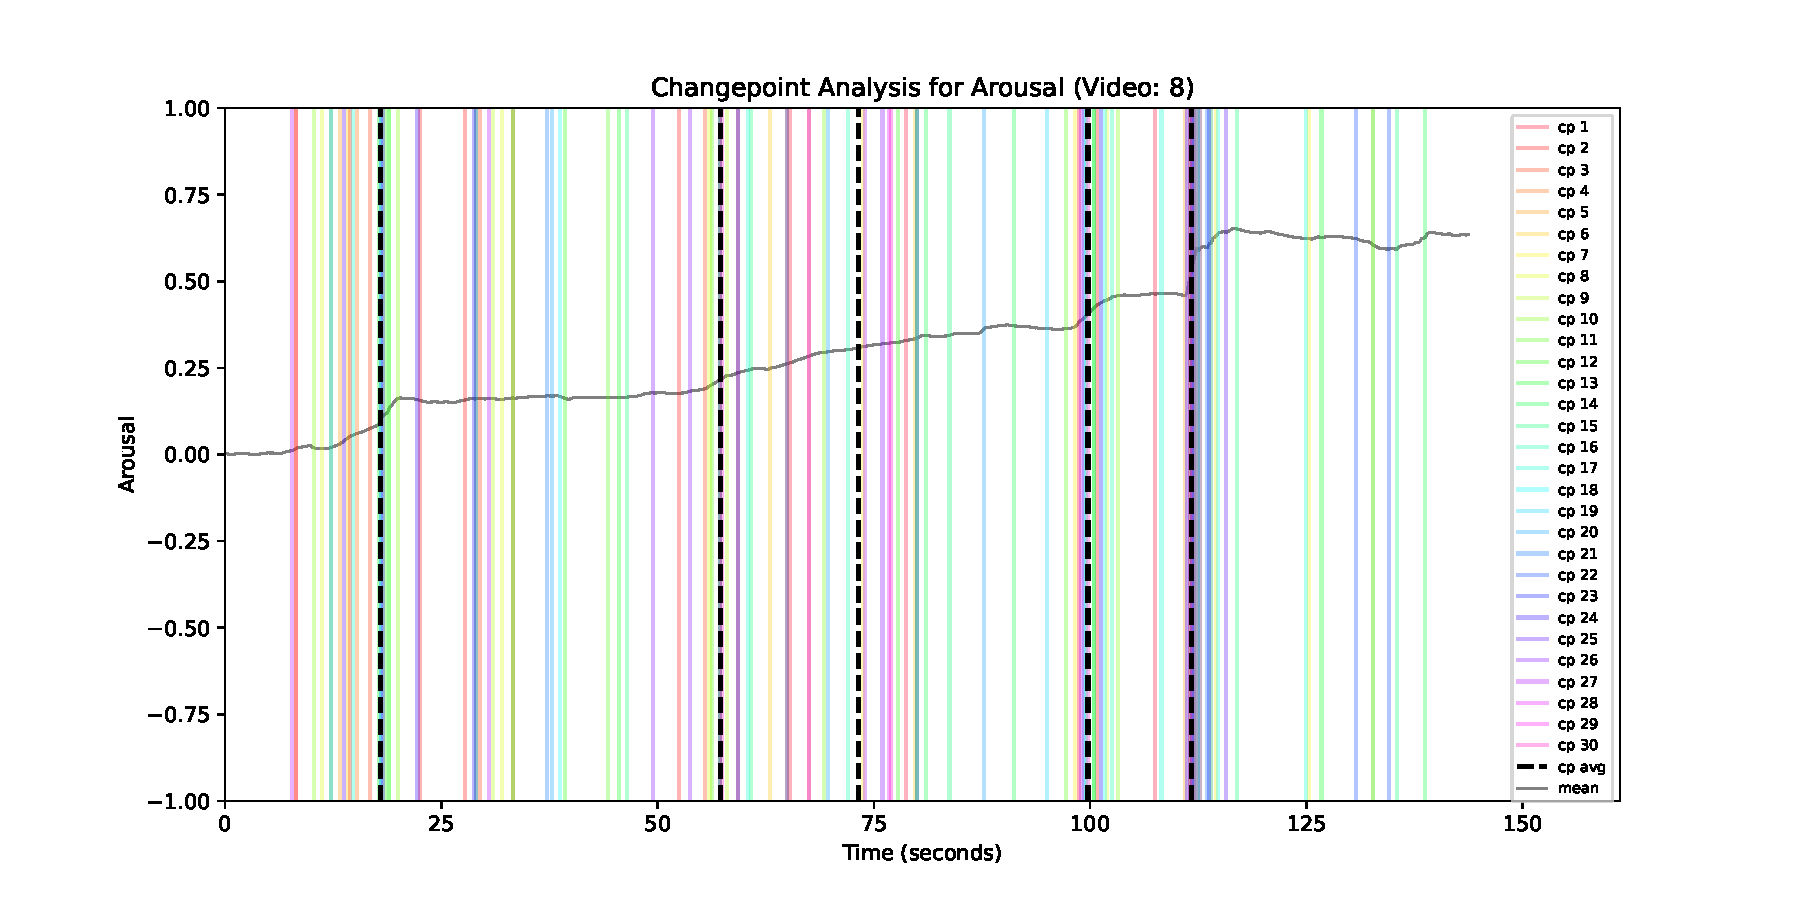
\includegraphics[width=\linewidth]{changepoints_V8_arousal_avg} 
        \caption{} \label{fig:changepoints_V8_arousal_avg}
    \end{subfigure}
    \hfill
    \begin{subfigure}[t]{0.49\textwidth}
        \centering
        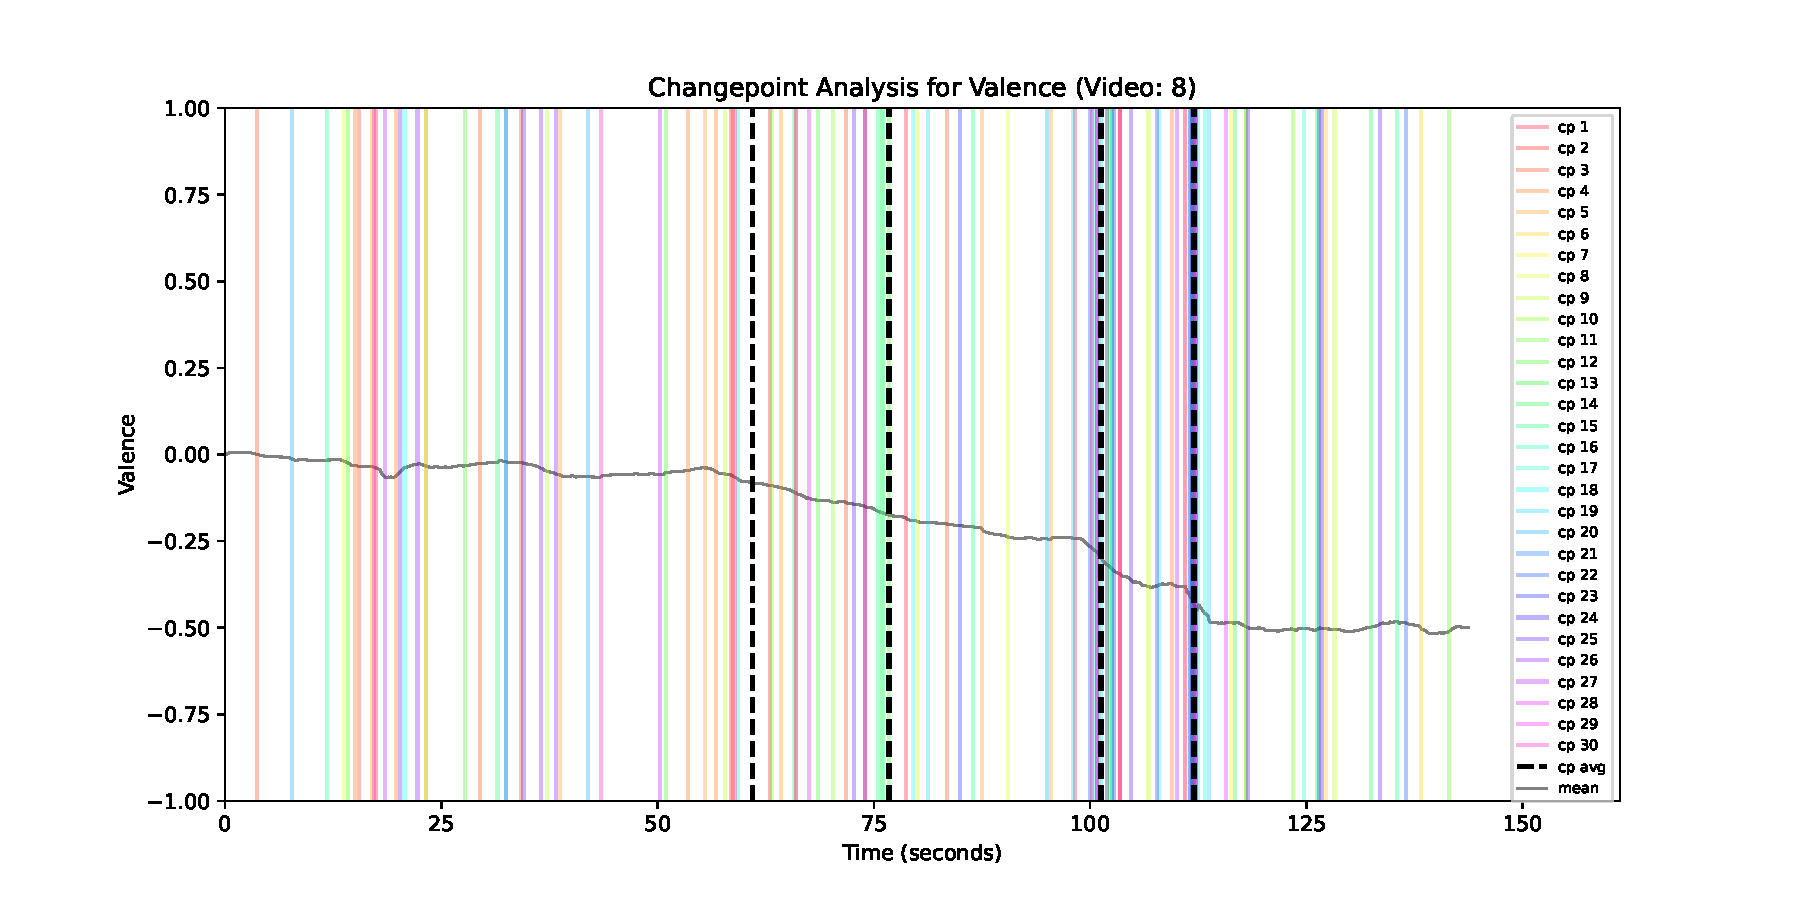
\includegraphics[width=\linewidth]{changepoints_V8_valence_avg} 
        \caption{} \label{fig:changepoints_V8_valence_avg}
    \end{subfigure}
    
    \caption{\textit{Change points in arousal and valence ratings for all videos for all subjects} Change points as identified by the algorithm for each video's arousal (left column) and valence (right column) ratings for all subjects. Thin colored lines indicate the subjects' change points. Black dashed lines indicate the mean change points. The thin grey line is the mean time series.There seem to be great interindividual differences. Only in video 7 and video 8, participants' alignment seemed to be higher. Note the different lengths of the videos.}
    \label{fig:all}
\end{figure}

% ----------------------------------------------------- code and figure availability ---------------------------------------------------------------
\section{Code and Figure Availability} \label{code}
All python scripts can be found on GitHub: 
\url{https://github.com/lucyroe/AVR_CPA}.
All figures depicted here can also be found separately on OwnCloud in the AffectiveVR directory.

\end{document}